\documentclass[]{book}
\usepackage{lmodern}
\usepackage{amssymb,amsmath}
\usepackage{ifxetex,ifluatex}
\usepackage{fixltx2e} % provides \textsubscript
\ifnum 0\ifxetex 1\fi\ifluatex 1\fi=0 % if pdftex
  \usepackage[T1]{fontenc}
  \usepackage[utf8]{inputenc}
\else % if luatex or xelatex
  \ifxetex
    \usepackage{mathspec}
  \else
    \usepackage{fontspec}
  \fi
  \defaultfontfeatures{Ligatures=TeX,Scale=MatchLowercase}
\fi
% use upquote if available, for straight quotes in verbatim environments
\IfFileExists{upquote.sty}{\usepackage{upquote}}{}
% use microtype if available
\IfFileExists{microtype.sty}{%
\usepackage{microtype}
\UseMicrotypeSet[protrusion]{basicmath} % disable protrusion for tt fonts
}{}
\usepackage[margin=1in]{geometry}
\usepackage{hyperref}
\hypersetup{unicode=true,
            pdftitle={Case Studies in Reproducible Research: a spring seminar at UCSC},
            pdfauthor={Eric C. Anderson, Kristen C. Ruegg, Tina Cheng, and the students of EEB 295},
            pdfborder={0 0 0},
            breaklinks=true}
\urlstyle{same}  % don't use monospace font for urls
\usepackage{natbib}
\bibliographystyle{apalike}
\usepackage{color}
\usepackage{fancyvrb}
\newcommand{\VerbBar}{|}
\newcommand{\VERB}{\Verb[commandchars=\\\{\}]}
\DefineVerbatimEnvironment{Highlighting}{Verbatim}{commandchars=\\\{\}}
% Add ',fontsize=\small' for more characters per line
\usepackage{framed}
\definecolor{shadecolor}{RGB}{248,248,248}
\newenvironment{Shaded}{\begin{snugshade}}{\end{snugshade}}
\newcommand{\KeywordTok}[1]{\textcolor[rgb]{0.13,0.29,0.53}{\textbf{{#1}}}}
\newcommand{\DataTypeTok}[1]{\textcolor[rgb]{0.13,0.29,0.53}{{#1}}}
\newcommand{\DecValTok}[1]{\textcolor[rgb]{0.00,0.00,0.81}{{#1}}}
\newcommand{\BaseNTok}[1]{\textcolor[rgb]{0.00,0.00,0.81}{{#1}}}
\newcommand{\FloatTok}[1]{\textcolor[rgb]{0.00,0.00,0.81}{{#1}}}
\newcommand{\ConstantTok}[1]{\textcolor[rgb]{0.00,0.00,0.00}{{#1}}}
\newcommand{\CharTok}[1]{\textcolor[rgb]{0.31,0.60,0.02}{{#1}}}
\newcommand{\SpecialCharTok}[1]{\textcolor[rgb]{0.00,0.00,0.00}{{#1}}}
\newcommand{\StringTok}[1]{\textcolor[rgb]{0.31,0.60,0.02}{{#1}}}
\newcommand{\VerbatimStringTok}[1]{\textcolor[rgb]{0.31,0.60,0.02}{{#1}}}
\newcommand{\SpecialStringTok}[1]{\textcolor[rgb]{0.31,0.60,0.02}{{#1}}}
\newcommand{\ImportTok}[1]{{#1}}
\newcommand{\CommentTok}[1]{\textcolor[rgb]{0.56,0.35,0.01}{\textit{{#1}}}}
\newcommand{\DocumentationTok}[1]{\textcolor[rgb]{0.56,0.35,0.01}{\textbf{\textit{{#1}}}}}
\newcommand{\AnnotationTok}[1]{\textcolor[rgb]{0.56,0.35,0.01}{\textbf{\textit{{#1}}}}}
\newcommand{\CommentVarTok}[1]{\textcolor[rgb]{0.56,0.35,0.01}{\textbf{\textit{{#1}}}}}
\newcommand{\OtherTok}[1]{\textcolor[rgb]{0.56,0.35,0.01}{{#1}}}
\newcommand{\FunctionTok}[1]{\textcolor[rgb]{0.00,0.00,0.00}{{#1}}}
\newcommand{\VariableTok}[1]{\textcolor[rgb]{0.00,0.00,0.00}{{#1}}}
\newcommand{\ControlFlowTok}[1]{\textcolor[rgb]{0.13,0.29,0.53}{\textbf{{#1}}}}
\newcommand{\OperatorTok}[1]{\textcolor[rgb]{0.81,0.36,0.00}{\textbf{{#1}}}}
\newcommand{\BuiltInTok}[1]{{#1}}
\newcommand{\ExtensionTok}[1]{{#1}}
\newcommand{\PreprocessorTok}[1]{\textcolor[rgb]{0.56,0.35,0.01}{\textit{{#1}}}}
\newcommand{\AttributeTok}[1]{\textcolor[rgb]{0.77,0.63,0.00}{{#1}}}
\newcommand{\RegionMarkerTok}[1]{{#1}}
\newcommand{\InformationTok}[1]{\textcolor[rgb]{0.56,0.35,0.01}{\textbf{\textit{{#1}}}}}
\newcommand{\WarningTok}[1]{\textcolor[rgb]{0.56,0.35,0.01}{\textbf{\textit{{#1}}}}}
\newcommand{\AlertTok}[1]{\textcolor[rgb]{0.94,0.16,0.16}{{#1}}}
\newcommand{\ErrorTok}[1]{\textcolor[rgb]{0.64,0.00,0.00}{\textbf{{#1}}}}
\newcommand{\NormalTok}[1]{{#1}}
\usepackage{longtable,booktabs}
\usepackage{graphicx,grffile}
\makeatletter
\def\maxwidth{\ifdim\Gin@nat@width>\linewidth\linewidth\else\Gin@nat@width\fi}
\def\maxheight{\ifdim\Gin@nat@height>\textheight\textheight\else\Gin@nat@height\fi}
\makeatother
% Scale images if necessary, so that they will not overflow the page
% margins by default, and it is still possible to overwrite the defaults
% using explicit options in \includegraphics[width, height, ...]{}
\setkeys{Gin}{width=\maxwidth,height=\maxheight,keepaspectratio}
\IfFileExists{parskip.sty}{%
\usepackage{parskip}
}{% else
\setlength{\parindent}{0pt}
\setlength{\parskip}{6pt plus 2pt minus 1pt}
}
\setlength{\emergencystretch}{3em}  % prevent overfull lines
\providecommand{\tightlist}{%
  \setlength{\itemsep}{0pt}\setlength{\parskip}{0pt}}
\setcounter{secnumdepth}{5}
% Redefines (sub)paragraphs to behave more like sections
\ifx\paragraph\undefined\else
\let\oldparagraph\paragraph
\renewcommand{\paragraph}[1]{\oldparagraph{#1}\mbox{}}
\fi
\ifx\subparagraph\undefined\else
\let\oldsubparagraph\subparagraph
\renewcommand{\subparagraph}[1]{\oldsubparagraph{#1}\mbox{}}
\fi

%%% Use protect on footnotes to avoid problems with footnotes in titles
\let\rmarkdownfootnote\footnote%
\def\footnote{\protect\rmarkdownfootnote}

%%% Change title format to be more compact
\usepackage{titling}

% Create subtitle command for use in maketitle
\newcommand{\subtitle}[1]{
  \posttitle{
    \begin{center}\large#1\end{center}
    }
}

\setlength{\droptitle}{-2em}
  \title{Case Studies in Reproducible Research: a spring seminar at UCSC}
  \pretitle{\vspace{\droptitle}\centering\huge}
  \posttitle{\par}
  \author{Eric C. Anderson, Kristen C. Ruegg, Tina Cheng, and the students of EEB
295}
  \preauthor{\centering\large\emph}
  \postauthor{\par}
  \predate{\centering\large\emph}
  \postdate{\par}
  \date{2017-05-12}

\usepackage{booktabs}
\usepackage{amsthm}
\makeatletter
\def\thm@space@setup{%
  \thm@preskip=8pt plus 2pt minus 4pt
  \thm@postskip=\thm@preskip
}
\makeatother

\usepackage{amsthm}
\newtheorem{theorem}{Theorem}[chapter]
\newtheorem{lemma}{Lemma}[chapter]
\theoremstyle{definition}
\newtheorem{definition}{Definition}[chapter]
\newtheorem{corollary}{Corollary}[chapter]
\newtheorem{proposition}{Proposition}[chapter]
\theoremstyle{definition}
\newtheorem{example}{Example}[chapter]
\theoremstyle{remark}
\newtheorem*{remark}{Remark}
\begin{document}
\maketitle

{
\setcounter{tocdepth}{1}
\tableofcontents
}
\chapter{Course Overview}\label{course-overview}

This is the home of the notes for a proposed course in data analysis and
reproducible research using R, Rstudio, and GitHub.

The seminar is called, ``Case Studies in Reproducible Research,'' but we
utter that title with the caveat that, although the organizers have
quite a few case studies they could spin up for this course, the case
studies we will be studying in this course are going to be actual
research projects that \emph{you}---the participants---are working on.
You're gonna bring 'em, and we are going to collectively help you
wrassle them into a reasonable and reproducible data analysis. In the
process we will touch on a number of elements of data analysis with R.

We will be working through a healthy chunk of the material in Garrett
Grolemund and Hadley Wickham's book, \href{http://r4ds.had.co.nz/}{R for
Data Science}, which is readable for free at the link above. We intend
to use a handful of our own data sets each week to illustrate points
from the book and show the material in action on real data sets.

This is not intended as a ``first course in R''. Students coming to the
course should have at least a modicum of familiarity with using R, and
we will launch more directly into using the tools of the
\href{http://tidyverse.org/}{tidyverse}. EEB students with little or no
experience in R might be interested in sitting in with Giacomo
Bernardi's lab group on Mondays at 3PM in the COH library. They are
conducting a Bio 295 seminar, working through ``a super basic book that
takes the very first steps into R.''

For the interested, these materials were all prepared using RStudio's
\href{https://bookdown.org/}{bookdown} package. The RStudio project in
which it lives is hosted on eriq's GitHub page
\href{https://github.com/eriqande/rep-res-eeb-2017}{here}

\section{Meeting Times, Location,
Requirements}\label{meeting-times-location-requirements}

Intended to be Friday afternoons, 1:45--3:15 PM in the
library/conference room at Long Marine Lab.

Students must bring a laptop to do examples during the seminar, and all
students are expected to have a data set that they are in the midst of
analyzing (or upon which they hope to commence analysis soon!) for a
research project. We will

\section{The origin of this seminar}\label{the-origin-of-this-seminar}

The idea for this course was floated by Tina Cheng who was planning to
lead a seminar in spring 2017 based in part on Eric C. Anderson's
\href{http://eriqande.github.io/rep-res-web/}{``Reproducible Research
Course''}, taught at the Southwest Fisheries Science Center in the fall
of 2014. Although going over those notes might have been a reasonable
exercise, it turns out that a lot has changed in the world of data
analysis since fall 2014, and the notes from that course are, today, a
little bit dated.

We have been particularly excited by the ascendancy of Hadley Wickham's
\href{http://tidyverse.org/}{tidyverse} approach to data analysis, and
the tremendous development of a variety of tools developed by
\href{https://www.rstudio.com/}{RStudio} for integrating report
generation and data analysis into reproducible workflows. In fact, Eric
has been saying for the last year that if he were to teach another
course on data analysis it would be structured completely differently
than his \href{http://eriqande.github.io/rep-res-web/}{``Reproducible
Research Course''}. So, it was clearly time for him to stop talking and
help put together an updated and different course.

At the same time, in working on our own projects and in helping others,
we have consistently found that the most effective way for anyone to
learn data analysis is to ensure that it is immediately relevant to
whatever ongoing research project is currently consuming them.
Therefore, in the current seminar, we are hoping to spend at least half
of our time ``workshopping'' the data sets that seminar participants are
actually involved in analyzing. Together we will help students wrestle
their data, analyses, and ideas into a single, well-organized RStudio
project under version control with git. Therefore, every student should
come to this course with a data set and an associated analysis project.

\section{Course Organizers}\label{course-organizers}

\begin{description}
\item[Kristen C. Ruegg]
Kristen is a conservation geneticist who specializes in the application
of genome-wide data to understand population level processes and inform
management, with a particular focus on migratory birds. She has has been
enlightened to the powers of the ``tidyverse'' over the last couple of
years (mostly through the constant insistence of her enthusiastic
husband Eric Anderson) and is looking forward to becoming more fluid in
its application over the course of the quarter. Her main role in this
course will be to help with the course design and logistics and help
reign Eric in when he has started to orbit into some obscure realm of
statistical nuance.
\item[Eric C. Anderson]
Eric trained as a statistician who specializes in genetic data. Since
2003 he has worked at the NMFS Southwest Fisheries Science Center in
Santa Cruz. Although much of his statistical research involves the
development of computationally intensive methods for specialized
analyses of genetic data, he has been involved in a variety of data
analysis projects at NMFS and with collaborators worldwide. Eric was an
early adherent to reproducible research principles and continues, as
such, performing most of his research and data analysis in the open and
publicly available on GitHub (find his GitHub page
\href{https://github.com/eriqande}{here}). In 2014, he taught the
\href{http://eriqande.github.io/rep-res-web/}{``Reproducible Research
Course''} at NMFS, and is excited to provide an updated version,
focusing more, this time, on the recently developed ``tidyverse''.
\item[Tina Cheng]
Tina is a graduate student in EEB. She is going to be leading the
session during the first week of the course when Kristen and Eric are
still on spring break, and then she is going to be joining in on the fun
with us for the remainder of the quarter until she has to travel off to
Baja, TA-ing the ``supercourse'' during the last four weeks of the
quarter.
\end{description}

\section{Course Goals}\label{course-goals}

The goal of this course is for scientists, researchers, and students to
learn to:

\begin{itemize}
\tightlist
\item
  properly store, manage, and distribute their data in a \emph{tidy}
  format
\item
  consolidate their digital research materials and analyses into
  well-organized RStudio projects.
\item
  use the tools of the tidyverse to manipulate and analyze those data
  sets
\item
  integrate data analysis with report generation and article preparation
  using the Rmarkdown format and using
  \href{http://rmarkdown.rstudio.com/r_notebooks.html}{R Notebooks}
\item
  use git version control software and GitHub to effectively manage data
  and source code, collaborate efficiently with other researchers, and
  neatly package their research.
\end{itemize}

By the end of the course, the hope is that we will all have mastered
strategies allowing us to use the above-listed, freely-available and
open-source tools for conducting research in a reproducible fashion. The
ideal we will be striving for is to be able to start from a raw data set
and then write a computer program that conducts all the cleaning,
manipulation, and analysis of the data, and presentation of the results,
in an automated fashion. Carrying out analysis and report-generation in
this way carries a number of advantages to the researcher:

\begin{enumerate}
\def\labelenumi{\arabic{enumi}.}
\tightlist
\item
  Newly-collected data can be integrated easily into your analysis.
\item
  If a mistake is found in one section of your analysis, it is not
  terribly onerous to correct it and then re-run all the downstream
  analyses.
\item
  Revising a manuscript to address referee comments can be done quickly.
\item
  Years after publication, the exact steps taken to analyze the data
  will still be available should anyone ask you how, exactly, you did an
  analysis!
\item
  If you have to conduct similar analyses and produce similar reports on
  a regular bias with new data each time, you might be able to do this
  readily by merely updating your data and then automatically producing
  the entire report.
\item
  If someone finds an error in your work, they can fix it and then
  easily show you exactly what they did to fix it.
\end{enumerate}

Additionally, packaging one's research in a reproducible fashion is
beneficial to the research community. Others that would like to confirm
your results can do so easily. If someone has concerns about exactly how
a particular analysis was carried out, they can find the precise details
in the code that you wrote to do it. Someone wanting to apply your
methods to their own data can easily do so, and, finally, if we are all
transparent and open about the methods that we use, then everyone can
learn more quickly from their colleagues.

In many fields today, publication of research requires the submission of
the original data to a publicly-available data repository. Currently,
several journals require that all analyses be packaged in a clear and
transparent fashion for easy reproduction of the results, and I predict
that trend will continue until most, if not all, journals will require
that data analyses be available in easily reproduced formats. This
course will help scientists prepare themselves for this eventuality. In
the process, you will probably find that conducting your research in a
reproducible fashion helps you work more efficiently (and perhaps even
more enjoyably!)

\section{Weekly Syllabus}\label{weekly-syllabus}

\subsection{Week 1 --- Introduction and Getting Your Workspace Set
Up}\label{week-1-introduction-and-getting-your-workspace-set-up}

\begin{itemize}
\tightlist
\item
  At the end of this session we want to make sure that everyone has R,
  RStudio, and Git installed on their systems, and that they are working
  as expected.
\item
  Additionally, everyoneshould have a free account on GitHub.
\item
  And finally we need everyone's email address.
\end{itemize}

Some things to do:

\begin{itemize}
\tightlist
\item
  Get Rstudio cheat Sheets!
\item
  Assemble data into a project
\item
  Get private GitHub repos
\end{itemize}

Eric! You need to make an example project repo.

\subsection{Week 2 --- RStudio project organization; using git and
GitHub; Quick
RMarkdown}\label{week-2-rstudio-project-organization-using-git-and-github-quick-rmarkdown}

After this, students are going to have to put their own data into their
own repositories and write a README.Rmd and make a README.md out of it.

\subsection{Week 3 --- Tibbles. Reading data in. Data
rectangling}\label{week-3-tibbles.-reading-data-in.-data-rectangling}

\begin{itemize}
\tightlist
\item
  Reading data into the data frames.
\item
  read.table and read.csv
\item
  tibbles
\item
  The readr package
\item
  Data types in the different columns and quick data sanity checks.
\item
  A few different gotcha's
\item
  Saving and reading data in R formats. \texttt{saveRDS} and
  \texttt{readRDS}.
\end{itemize}

\subsection{Week 4 ---}\label{week-4}

\chapter{Week One Meeting}\label{week1}

Tina is going to be helping everyone get their systems all set up. After
that we will have everyone clone an RStudio project from GitHub to see
how easy that is.

\section{Software Installation}\label{software-installation}

\begin{enumerate}
\def\labelenumi{\arabic{enumi}.}
\item
  \textbf{RStudio:} We want the latest ``development'' version of
  RStudio becuase it has features that we may want to use during this
  course. Get it from
  \url{https://www.rstudio.com/products/rstudio/download/preview/} and
  install the appropriate one for your OS.
\item
  \textbf{R:} Let's make sure that we are all using the latest version
  of R. On March 7, 2017, version 3.3.3 was released. Go to
  \url{https://cran.r-project.org/} and find the download link for your
  computer system. Download it and install it.
\item
  \textbf{bookdown:} This package is what I used to create these course
  notes. Getting it automatically installs a lot of other packages that
  are useful for authoring reproducible research. We want the latest
  development version, which can be obtained from GitHub by issuing the
  following commans at the R prompt (i.e.~in the console window of
  RStudio:)

\begin{Shaded}
\begin{Highlighting}[]
\KeywordTok{install.packages}\NormalTok{(}\StringTok{"devtools"}\NormalTok{)  }
\NormalTok{devtools::}\KeywordTok{install_github}\NormalTok{(}\StringTok{"rstudio/bookdown"}\NormalTok{)}
\end{Highlighting}
\end{Shaded}
\item
  Install \textbf{other packages} that we are going to be needing in the
  first few weeks. If you don't know how to install packages, ask Tina
  and she can show you. Install: \texttt{tidyverse}, and
  \texttt{stringr}.
\item
  Make sure that \textbf{git} is up and running on your system.

  \begin{itemize}
  \item
    If you are using a Mac with a reasonably new OS, you should be able
    to just open the Terminal application
    (\texttt{/Applications/Utilities/Terminal}) and type ``git'' at the
    command line. If you have \texttt{git} it will say something that
    starts like:

\begin{Shaded}
\begin{Highlighting}[]
    \KeywordTok{usage}\NormalTok{: git [--version] [--help] [-C }\KeywordTok{<}\NormalTok{path}\KeywordTok{>}\NormalTok{] [-c name=value]}
   \NormalTok{[}\KeywordTok{--exec-path}\NormalTok{[=}\KeywordTok{<}\NormalTok{path}\KeywordTok{>}\NormalTok{]] [--html-path] [--man-path] [--info-path]}
   \NormalTok{[}\KeywordTok{-p} \KeywordTok{|} \KeywordTok{--paginate} \KeywordTok{|} \KeywordTok{--no-pager}\NormalTok{] [--no-replace-objects] [--bare]}
   \NormalTok{[}\KeywordTok{--git-dir}\NormalTok{=}\KeywordTok{<}\NormalTok{path}\KeywordTok{>}\NormalTok{] [--work-tree=}\KeywordTok{<}\NormalTok{path}\KeywordTok{>}\NormalTok{] [--namespace=}\KeywordTok{<}\NormalTok{name}\KeywordTok{>}\NormalTok{]}
   \KeywordTok{<command>} \NormalTok{[}\KeywordTok{<}\NormalTok{args}\KeywordTok{>}\NormalTok{]}

\KeywordTok{These} \NormalTok{are common Git commands used in various situations:}

\KeywordTok{start} \NormalTok{a working area (see also: git help tutorial)}
   \KeywordTok{clone}      \NormalTok{Clone a repository into a new directory}
   \KeywordTok{etc.} \NormalTok{etc. etc.}
\end{Highlighting}
\end{Shaded}

    If you do not have \texttt{git} then it should pop up a little thing
    asking if you would like to install a reduced set of developer
    tools. You do. Click OK. \textbf{NOTE} Instead of a pop up it might
    say something like, ``xcrun Error: invalid active developer path.
    etc. etc\ldots{}''. In that case, you can install a fresh set of
    command line tools by typing this at the command line:

\begin{verbatim}
xcode-select --install
\end{verbatim}
  \item
    If you are using a PC, I can't be as much help, but you can find
    links with instructions on how to download \texttt{git} for a PC
    \href{https://support.rstudio.com/hc/en-us/articles/200532077-Version-Control-with-Git-and-SVN}{here}.
  \item
    If you are using Linux then we will assume you know how to get
    \texttt{git} or that you already have it.
  \end{itemize}
\end{enumerate}

\section{Get an account on GitHub}\label{get-an-account-on-github}

If you don't already have an account on GitHub, go to \url{github.com}
and click the ``sign up'' link near upper right of the page. It is
pretty self-explanatory. Go ahead and get a \textbf{free} account. There
is nothing to pay for here!

\subsection{Private repositories}\label{private-repositories}

\emph{If you are a graduate student} and you do not feel comfortable
posting your data on a public site like GitHub, then you should request
some private repositories from GitHub. GitHub has a great deal for
academic users like students: free private repositories. Please go to
\url{https://education.github.com/pack} to sign up for your free student
pack.

\section{Open an RStudio Project from
GitHub}\label{open-an-rstudio-project-from-github}

I am going to have everyone use RStudio and GitHub to clone and open an
RStudio project that I prepared as a template so that people can see how
I would like them to start putting together their own projects.

To open this project, from RStudio, go to the menu option
``File-\textgreater{}New Project\ldots{}''. Then from the resulting
dialog, choose ``Version Control''. Then choose ``Git''. Then it asks
for a ``repository URL''. Supply this:
\texttt{https://github.com/eriqande/rep-res-coho-example} and leave the
``Project Directory Name'' empty. And then choose a directory in which
to put it and click OK.

Bam! That will pull the RStudio project off of GitHub, make a local
clone of it on your hard drive and open.

Once you have done that. Open \texttt{README.Rmd} within the project,
and click the ``knit'' button which should be present near the top left
of the editor window.

That is how you convert an R Markdown README to README.md which is easy
to read and see on GitHub.

If you want to see what the project repository looks like on GitHub,
have a look at \url{https://github.com/eriqande/rep-res-coho-example}.

\section{Assignment for next week: Create an RStudio Project with Your
Own
Data}\label{assignment-for-next-week-create-an-rstudio-project-with-your-own-data}

Your mission for the following week---i.e., please have this done (or as
done as you can get it) by Friday, April 14, 2017---is to prepare an
RStudio project with your own data set, and provide some background
about the data and the ways that you would like to analyze it. The
``rep-res-coho-example'' is an example of what I have in mind for this.
You should use the README.Rmd from that project as a template for your
own README.Rmd. (To do this you can just copy the README.Rmd file into
the top level of your project directory and then edit it to reflect your
own data and project.)

To do all this you are going to want to make your own project. Do that
like this:

\begin{enumerate}
\def\labelenumi{\arabic{enumi}.}
\tightlist
\item
  In RStudio, choose ``File-\textgreater{}New Project\ldots{}''
\item
  Then choose ``New Directory'' and then choose ``Empty Project''
\item
  In the next dialog, choose a name (\emph{it is best to use only
  letters, numbers, dashes, and underscores, and include no spaces in
  the name}) for it \textbf{and be sure to click the ``Create a git
  repository'' button}.\\
\item
  Then click ``Create Project''.
\end{enumerate}

That should give you a new project. Here are some guidelines for putting
your own data in there

\begin{itemize}
\tightlist
\item
  Put all of your data in a directory named \texttt{data} in your
  project.
\item
  CSV (comma separated values) is probably the best format to use. It is
  text-readable without proprietary software (unlike an Excel file);
  however if you need to look at it in a tabular way with Excel, (gasp),
  you can do that easily. Tab-delimited text works if you have that, but
  CSV is preferred.
\item
  Use only letters, numbers, dashes, and underscores for the file names,
  (and periods for their extensions, i.e., \texttt{.csv})
\item
  Give a brief description of your data in the README.Rmd.
\end{itemize}

\section{Reading for next week}\label{week2reading}

This week (before Friday, April 14, 2017), please read the following
sections of the R for Data Science book

\begin{itemize}
\tightlist
\item
  \href{http://r4ds.had.co.nz/workflow-basics.html}{Workflow basics}:
  super basic review on how R works.
\item
  \href{http://r4ds.had.co.nz/workflow-projects.html}{Workflow:
  projects}: info about organizing RStudio projects.
\item
  \href{http://r4ds.had.co.nz/workflow-scripts.html}{Workflow: scripts}:
  how to evaluate code in scripts.
\item
  \href{http://r4ds.had.co.nz/tibbles.html}{tibbles}: a streamlined data
  frame format.
\item
  \href{http://r4ds.had.co.nz/data-import.html}{data import} This is our
  key reading for the week.
\end{itemize}

When you are done with the \emph{Data Import} reading, take a whack at
writing some code to read the data files in your project into a variable
(or several variables).

\chapter{Week Two Meeting}\label{week2}

For this week, everyone should have completed the reading listed in
Section \ref{week2reading}. And everyone should have at least been
trying to set up an RStudio Project with their own data in it, and given
a whack at reading their data into a variable.

\section{Workflow and Project Recap}\label{workflow-and-project-recap}

\subsection{Workflow: basics}\label{workflow-basics}

\subsubsection{Style}\label{style}

I just want to reiterate a few things that might seem minor, but are
stylistically important in the long run.

\begin{enumerate}
\def\labelenumi{\arabic{enumi}.}
\tightlist
\item
  Don't use \texttt{=} for assignment. Use \texttt{\textless{}-}. On a
  Mac use Option-``-'' to get that more quickly.

  \begin{itemize}
  \item
    Hey! Note that you \emph{do} use \texttt{=} (and \textbf{only}
    \texttt{=}) for \emph{passing values to function arguments}.

\begin{Shaded}
\begin{Highlighting}[]
\CommentTok{# do this:}
\NormalTok{my_variable <-}\StringTok{ }\DecValTok{10}

\CommentTok{# don't do this (it works but is not good style)}
\NormalTok{my_variable =}\StringTok{ }\DecValTok{10}


\CommentTok{# do this}
\NormalTok{result <-}\StringTok{ }\KeywordTok{my_function}\NormalTok{(}\DataTypeTok{arg1 =} \DecValTok{10}\NormalTok{, }\DataTypeTok{arg2 =} \StringTok{"foo"}\NormalTok{)}

\CommentTok{# don't do this (it might return a results, but will likely be incorrect)}
\NormalTok{result <-}\StringTok{ }\KeywordTok{my_function}\NormalTok{(arg1 <-}\StringTok{ }\DecValTok{10}\NormalTok{, arg2 <-}\StringTok{ "foo"}\NormalTok{)}

\CommentTok{# for example, figure out how this fails:}
\KeywordTok{matrix}\NormalTok{(data <-}\StringTok{ }\DecValTok{1}\NormalTok{:}\DecValTok{10}\NormalTok{, nrow <-}\StringTok{ }\DecValTok{5}\NormalTok{, byrow <-}\StringTok{ }\OtherTok{TRUE}\NormalTok{)}
\end{Highlighting}
\end{Shaded}
  \end{itemize}
\item
  Put spaces around both sides of \texttt{=}, and \texttt{\textless{}-},
  and other mathematical operators like \texttt{+}, \texttt{-},
  \texttt{*}, etc.
\item
  Put spaces after commas.
\item
  Use R-Studio's magical \texttt{Cmd-i} keyboard shortcut to
  automatically indent highlighted code.
\item
  If you want to really geek out, Hadley shares his style tips more
  completely in his \href{http://adv-r.had.co.nz/Style.html}{Advanced R
  Programming} book.
\item
  In fact, he now has updated those edicts for the tidyverse
  \href{http://style.tidyverse.org/index.html}{here}.
\end{enumerate}

This might seem pedantic, but adhering to these conventions makes it
much easier for people to read your code.

\subsubsection{TAB-completion}\label{tab-completion}

This is HUGE!! Start developing a twitchy left pinky now!

TAB early; TAB often!

Note that that completions of R code in the console or in the source
window are context dependent:

\begin{itemize}
\tightlist
\item
  variables in global environment
\item
  Functions
\item
  Quoted strings complete to filenames in directories
\item
  Installed packages in \texttt{library()}
\item
  Help topics after \texttt{?}
\item
  Function arguments within a function's parentheses. This is absolutely
  huge. If you can't remember all the different arguments a function
  takes, type the function and hit TAB within the parentheses. Try
  typing \texttt{read.table()} and his TAB while the cursor is inside
  the parentheses. Use the up and down arrows to scroll through the
  options, hit TAB again to insert one. Note that after you have used an
  argument it no longer appears in the list of options.
\end{itemize}

\subsubsection{Ctrl + Shift + 1/2/3/4 to turn one of the panes to
full-screen}\label{ctrl-shift-1234-to-turn-one-of-the-panes-to-full-screen}

Thanks to Diana for writing about practing that in her homework. Awesome
feature that I've not used previously!

\subsection{Workflow: projects}\label{workflow-projects}

\subsubsection{Disable saving of workspace for
sure!}\label{disable-saving-of-workspace-for-sure}

Let's all walk through this.

\subsubsection{Another worthwhile preference for small-screens (like
laptops)}\label{another-worthwhile-preference-for-small-screens-like-laptops}

Make sure that the RMarkdown preference is set to open in:
\textbf{Window}. See Figure \ref{fig:rmd-window}.

\begin{figure}

{\centering 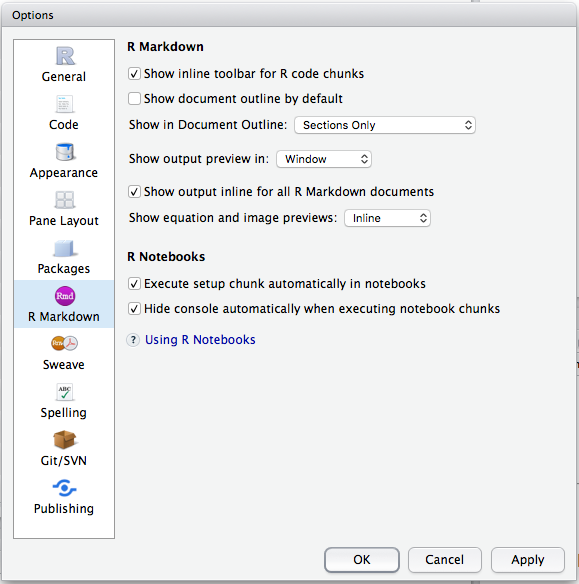
\includegraphics[width=0.9\linewidth]{images/rmd_window} 

}

\caption{To read RMarkdown output in a separate page (highly recommended for laptops) choose "RMarkdown" on the left and choose "Window" from the dropdown menu, and click OK.}\label{fig:rmd-window}
\end{figure}

\subsubsection{Opening RStudio Projects from the OS (by clicking in the
Finder)}\label{opening-rstudio-projects-from-the-os-by-clicking-in-the-finder}

\begin{itemize}
\tightlist
\item
  You can open an RStudio project by double clicking the RStudio Project
  icon from, for example, a Mac Finder window. It lives in a directory
  of the same name (but it has a \texttt{.Rproj} exension.)
\item
  Or if you are a command line type, use, for example
  \texttt{open\ my\_project.Rproj} from the Terminal.
\item
  You can open as many RStudio projects as you like at a time.
\item
  Each RStudio project launches its own, completely separate R session!
\item
  Interestingly, if you click on the \texttt{.Rproj} file of a project
  that is open, RStudio will open another instance of that project. So,
  don't click on the \texttt{.Rproj} file for a project that is already
  open!

  \begin{itemize}
  \tightlist
  \item
    (In other applications on the Mac that will typically just take you
    to the currently open docuemnt, but not so with RStudio.)
  \end{itemize}
\item
  Use cmd-TAB to switch between open RStudio projects.
\end{itemize}

\subsubsection{Opening RStudio Projects from
RStudio}\label{opening-rstudio-projects-from-rstudio}

\begin{itemize}
\tightlist
\item
  When you open existing projects using the ``File-\textgreater{}Open
  Project\ldots{}'' menu option or with the ``File -\textgreater{}
  Recent Projects'' menu option and you currently have RStudio open ``in
  another project,''" then the new project that you are opening jumps in
  ``on top of'' the previous one. It looks like your previous project
  has vanished into the ether. The OS thinks there is only one RStudio
  open, an it has the most recently opened project in it. WHERE'S MY
  OTHER ONE?!
\item
  You can get back to it by clicking the project dropdown in the upper
  right of the project.
\item
  However, if you switch between projects this way it restarts R each
  time you switch back to your project so it takes a lot of time and it
  is super-annoying.
\item
  If you are working concurrently in multiple projects, I recommend
  opening them from the Finder (or Terminal) and switching between them
  using \textbf{Cmd-TAB}.
\end{itemize}

\subsubsection{\texorpdfstring{What is the \texttt{.Rproj} file,
really}{What is the .Rproj file, really}}\label{what-is-the-.rproj-file-really}

It is just a text file that stores some information and any
project-specific preferences if there are any. Here is what
\texttt{rep-res-eeb-2017.Rproj} looks like if you open it with a text
editor:

\begin{Shaded}
\begin{Highlighting}[]
\FunctionTok{Version:} \NormalTok{1.0}

\FunctionTok{RestoreWorkspace:} \NormalTok{Default}
\FunctionTok{SaveWorkspace:} \NormalTok{Default}
\FunctionTok{AlwaysSaveHistory:} \NormalTok{Default}

\FunctionTok{EnableCodeIndexing:} \NormalTok{Yes}
\FunctionTok{UseSpacesForTab:} \NormalTok{Yes}
\FunctionTok{NumSpacesForTab:} \NormalTok{2}
\FunctionTok{Encoding:} \NormalTok{UTF-8}

\FunctionTok{RnwWeave:} \NormalTok{knitr}
\FunctionTok{LaTeX:} \NormalTok{pdfLaTeX}

\FunctionTok{AutoAppendNewline:} \NormalTok{Yes}
\FunctionTok{StripTrailingWhitespace:} \NormalTok{Yes}

\FunctionTok{BuildType:} \NormalTok{Website}
\end{Highlighting}
\end{Shaded}

\subsubsection{R in an RStudio project launches in the project
directory}\label{r-in-an-rstudio-project-launches-in-the-project-directory}

\begin{itemize}
\tightlist
\item
  This makes reproducibility much easier. You can find and load files
  using \emph{relative} paths.\\
\item
  Everything you might be accessing from R (data, scripts, etc.) or
  outputting from R will be easy to get to if they are ``in the
  project''
\item
  When we say that a file is ``in the project'' we mean that it is
  stored on disk somewhere within the project directory.
\item
  The project directory (sometimes called the \emph{root} of the project
  directory) is just the directory that contains the \texttt{.Rproj}
  file.
\item
  Expert user tip: \texttt{rprojroot::find\_rstudio\_root\_file()} (part
  of the \texttt{rprojroot} package) let's you find the root of an
  RStudio project directory. This can be helpful sometimes\ldots{}.
\end{itemize}

\subsection{Workflow: scripts}\label{workflow-scripts}

\begin{itemize}
\tightlist
\item
  Script editor window vs console window
\item
  Keyboard shortcuts for evaluating codes in your scripts:

  \begin{itemize}
  \tightlist
  \item
    \textbf{Cmd-Return} (sends current line to console and advances
    cursor to next line)
  \item
    \textbf{Highlight with Cmd-Return} (send highlighted code to
    console)

    \begin{itemize}
    \tightlist
    \item
      For this, \textbf{Shift-up-arrow} and \textbf{Shift-down-arrow}
      are good for highlighting.
    \item
      As is \textbf{Shift-Command-right-arrow} or
      \textbf{Shift-command-left-arrow}.
    \end{itemize}
  \end{itemize}
\end{itemize}

\section{\texorpdfstring{Let's talk about the pipe
\texttt{\%\textgreater{}\%}}{Let's talk about the pipe \%\textgreater{}\%}}\label{lets-talk-about-the-pipe}

For anyone who had ever worked comfortably in Unix for a long time, and
was used to chaining the output of one utility in as the input for
another utility using the pipe: \texttt{\textbar{}}, R's syntax for
composition of functions was always super cumbersome and required all
sorts of nasty, nested parentheses.

Consider this simple set of operations: imagine we want to

\begin{enumerate}
\def\labelenumi{\arabic{enumi}.}
\tightlist
\item
  simulate 1000 gamma random variables, \(G\), with parameters
  \(\alpha=5\) and \(\beta = 1\),
\item
  for each \(G\) simulate a Poisson random variable with mean
  (\texttt{lambda}) \(G\).
\item
  take the \texttt{sqrt} of each such variable
\item
  compute the variance of the result
\end{enumerate}

This can all be done in one line, but is ugly!

\begin{Shaded}
\begin{Highlighting}[]
\CommentTok{# set random seed for reproducibility}
\KeywordTok{set.seed}\NormalTok{(}\DecValTok{5}\NormalTok{)}

\KeywordTok{var}\NormalTok{(}\KeywordTok{sqrt}\NormalTok{(}\KeywordTok{rpois}\NormalTok{(}\DataTypeTok{n =} \DecValTok{1000}\NormalTok{, }\DataTypeTok{lambda =} \KeywordTok{rgamma}\NormalTok{(}\DataTypeTok{n =} \DecValTok{1000}\NormalTok{, }\DataTypeTok{shape =} \DecValTok{5}\NormalTok{, }\DataTypeTok{scale =} \DecValTok{1}\NormalTok{))))}
\end{Highlighting}
\end{Shaded}

\begin{verbatim}
## [1] 0.5828768
\end{verbatim}

It doesn't matter how stylishly you include spaces in your code, this is
just Fugly!

You can write it on multiple lines, but it is friggin' ghastly! Maybe
worse than before.

\begin{Shaded}
\begin{Highlighting}[]
\KeywordTok{set.seed}\NormalTok{(}\DecValTok{5}\NormalTok{)}

\KeywordTok{var}\NormalTok{(}
  \KeywordTok{sqrt}\NormalTok{(}
    \KeywordTok{rpois}\NormalTok{(}\DataTypeTok{n =} \DecValTok{1000}\NormalTok{, }\DataTypeTok{lambda =} \KeywordTok{rgamma}\NormalTok{(}
      \DataTypeTok{n =} \DecValTok{1000}\NormalTok{, }\DataTypeTok{shape =} \DecValTok{5}\NormalTok{, }\DataTypeTok{scale =} \DecValTok{1}
    \NormalTok{)}
    \NormalTok{)}
  \NormalTok{)}
\NormalTok{)}
\end{Highlighting}
\end{Shaded}

\begin{verbatim}
## [1] 0.5828768
\end{verbatim}

The problem is that the order in which the operations are done does not
match the way things are written: the first thing to get done is the
call to \texttt{rgamma}, which is nested deeply within the parentheses.

Enter the R ``pipe'' symbol. It is not as convenient to type as
\texttt{\textbar{}}, but you can make it quickly with the keyboard
shortcut \texttt{cmd-shift-M}: \texttt{\%\textgreater{}\%}. This was
introduced in the \texttt{magrittr} package, and the \texttt{tidyverse}
imports the \texttt{\%\textgreater{}\%} symbol from \texttt{magrittr}.

Behold!

\begin{Shaded}
\begin{Highlighting}[]
\KeywordTok{library}\NormalTok{(tidyverse)}
\KeywordTok{set.seed}\NormalTok{(}\DecValTok{5}\NormalTok{)}

\KeywordTok{rgamma}\NormalTok{(}\DataTypeTok{n =} \DecValTok{1000}\NormalTok{, }\DataTypeTok{shape =} \DecValTok{5}\NormalTok{, }\DataTypeTok{scale =} \DecValTok{1}\NormalTok{) %>%}
\StringTok{  }\KeywordTok{rpois}\NormalTok{(}\DataTypeTok{n =} \DecValTok{1000}\NormalTok{, }\DataTypeTok{lambda =} \NormalTok{.) %>%}\StringTok{          }\CommentTok{# pass G is as the lambda parameter using the dot: .}
\StringTok{  }\KeywordTok{sqrt}\NormalTok{() %>%}\StringTok{                               }\CommentTok{# no dot here, so the previous result is just the first argument to sqrt}
\StringTok{  }\KeywordTok{var}\NormalTok{()                                    }\CommentTok{# same here}
\end{Highlighting}
\end{Shaded}

\begin{verbatim}
## [1] 0.5828768
\end{verbatim}

That is a hell of a lot easier to read! It gives me goose bumps it is so
elegant.

The \texttt{\%\textgreater{}\%} symbol says, ``take the result that
occurred before the \texttt{\%\textgreater{}\%} and pass it in as the
\texttt{.} in whatever follows the \texttt{\%\textgreater{}\%}.''
Furthermore, if there is no \texttt{.} in the expression after the
\texttt{\%\textgreater{}\%}, simply pass the result that occurred before
the \texttt{\%\textgreater{}\%} in as the \emph{first argument} in the
function call that comes after the \texttt{\%\textgreater{}\%}.

This type of ``chaining'' of operations is particularly powerful when
operating on \texttt{tibbles} using \texttt{dplyr}

\section{\texorpdfstring{Tibbles and ``rectangular''
data}{Tibbles and rectangular data}}\label{tibbles-and-rectangular-data}

\begin{itemize}
\tightlist
\item
  gonna talk a little about data types too.
\item
  Chinook CWT data example.
\item
  Get comfy with the \texttt{View()} function!
\end{itemize}

\subsection{Tibble excercises}\label{tibble-excercises}

I'm gonna just blast through these here in case people are curious.
These are answers I would use.

\begin{enumerate}
\def\labelenumi{\arabic{enumi}.}
\item
  Use \texttt{class()}

\begin{Shaded}
\begin{Highlighting}[]
\KeywordTok{class}\NormalTok{(mtcars)}
\end{Highlighting}
\end{Shaded}

\begin{verbatim}
## [1] "data.frame"
\end{verbatim}

\begin{Shaded}
\begin{Highlighting}[]
\KeywordTok{class}\NormalTok{(tibble::}\KeywordTok{as_tibble}\NormalTok{(mtcars))}
\end{Highlighting}
\end{Shaded}

\begin{verbatim}
## [1] "tbl_df"     "tbl"        "data.frame"
\end{verbatim}

  Hey! does everyone see the \texttt{tibble::as\_tibble()} there? The
  \texttt{::} is the ``namespace addresser''. It lets you run a function
  from a library without loading the library. If you already have done
  \texttt{library(tidyverse)} you would have loaded the \texttt{tibble}
  library and could just write \texttt{as\_tibble(mtcars)} but I wanted
  to be explicit about where the \texttt{as\_tibble()} function comes
  from. (As an aside, it turns out that this is how you would write it
  if you were writing code for a package.)
\item
  Let's do it first as a \texttt{data.frame}:

\begin{Shaded}
\begin{Highlighting}[]
\KeywordTok{library}\NormalTok{(tidyverse)}
\NormalTok{df <-}\StringTok{ }\KeywordTok{data.frame}\NormalTok{(}\DataTypeTok{abc =} \DecValTok{1}\NormalTok{, }\DataTypeTok{xyz =} \StringTok{"a"}\NormalTok{)}
\NormalTok{df$x}
\end{Highlighting}
\end{Shaded}

\begin{verbatim}
## [1] a
## Levels: a
\end{verbatim}

\begin{Shaded}
\begin{Highlighting}[]
\NormalTok{df[, }\StringTok{"xyz"}\NormalTok{]}
\end{Highlighting}
\end{Shaded}

\begin{verbatim}
## [1] a
## Levels: a
\end{verbatim}

\begin{Shaded}
\begin{Highlighting}[]
\NormalTok{df[, }\KeywordTok{c}\NormalTok{(}\StringTok{"abc"}\NormalTok{, }\StringTok{"xyz"}\NormalTok{)]}
\end{Highlighting}
\end{Shaded}

\begin{verbatim}
##   abc xyz
## 1   1   a
\end{verbatim}

  And then we can do it again as a \texttt{tibble}

\begin{Shaded}
\begin{Highlighting}[]
\NormalTok{df <-}\StringTok{ }\KeywordTok{tibble}\NormalTok{(}\DataTypeTok{abc =} \DecValTok{1}\NormalTok{, }\DataTypeTok{xyz =} \StringTok{"a"}\NormalTok{) %>%}
\StringTok{  }\KeywordTok{as_tibble}\NormalTok{()}
\NormalTok{df$x}
\end{Highlighting}
\end{Shaded}

\begin{verbatim}
## Warning: Unknown or uninitialised column: 'x'.
\end{verbatim}

\begin{verbatim}
## NULL
\end{verbatim}

\begin{Shaded}
\begin{Highlighting}[]
\NormalTok{df$xyz}
\end{Highlighting}
\end{Shaded}

\begin{verbatim}
## [1] "a"
\end{verbatim}

\begin{Shaded}
\begin{Highlighting}[]
\NormalTok{df[, }\StringTok{"xyz"}\NormalTok{]}
\end{Highlighting}
\end{Shaded}

\begin{verbatim}
## # A tibble: 1 × 1
##     xyz
##   <chr>
## 1     a
\end{verbatim}

\begin{Shaded}
\begin{Highlighting}[]
\NormalTok{df[, }\KeywordTok{c}\NormalTok{(}\StringTok{"abc"}\NormalTok{, }\StringTok{"xyz"}\NormalTok{)]}
\end{Highlighting}
\end{Shaded}

\begin{verbatim}
## # A tibble: 1 × 2
##     abc   xyz
##   <dbl> <chr>
## 1     1     a
\end{verbatim}

  Aha! Things to notice are:

  \begin{enumerate}
  \def\labelenumii{\alph{enumii}.}
  \tightlist
  \item
    \texttt{data.frame()} coerces to factors.
  \item
    tibble doesn't do partial name matching
    \texttt{\$x}\(\neq\)\texttt{\$xyz}
  \item
    Square bracket extraction of a single column of a tibble retains its
    tibbleness. Not so with \texttt{data.frame}. With
    \texttt{data.frame} it gets turned into a vector.
  \item
    \texttt{\$} extraction with \texttt{tibble} returns a vector.
  \end{enumerate}
\item
  Let's make \texttt{mtcars} a \texttt{tibble}

\begin{Shaded}
\begin{Highlighting}[]
\NormalTok{mtcars_t <-}\StringTok{ }\KeywordTok{as_tibble}\NormalTok{(mtcars)}
\NormalTok{var <-}\StringTok{ "mpg"}

\CommentTok{# this will get the "mpg" column out but retain it as a tibble}
\NormalTok{mtcars_t[, var]}
\end{Highlighting}
\end{Shaded}

\begin{verbatim}
## # A tibble: 32 × 1
##      mpg
##    <dbl>
## 1   21.0
## 2   21.0
## 3   22.8
## 4   21.4
## 5   18.7
## 6   18.1
## 7   14.3
## 8   24.4
## 9   22.8
## 10  19.2
## # ... with 22 more rows
\end{verbatim}

\begin{Shaded}
\begin{Highlighting}[]
\CommentTok{# and this will just grab the column as a vector}
\NormalTok{mtcars_t[[var]]}
\end{Highlighting}
\end{Shaded}

\begin{verbatim}
##  [1] 21.0 21.0 22.8 21.4 18.7 18.1 14.3 24.4 22.8 19.2 17.8 16.4 17.3 15.2
## [15] 10.4 10.4 14.7 32.4 30.4 33.9 21.5 15.5 15.2 13.3 19.2 27.3 26.0 30.4
## [29] 15.8 19.7 15.0 21.4
\end{verbatim}
\item
  Remember that non-syntactic names (those that do not start with a
  letter or underscore and which include characters other than
  \texttt{-} and ``\_" and ``.'') must be enclosed in backticks. Let's
  get our data:

\begin{Shaded}
\begin{Highlighting}[]
\NormalTok{annoying <-}\StringTok{ }\KeywordTok{tibble}\NormalTok{(}
\StringTok{`}\DataTypeTok{1}\StringTok{`} \NormalTok{=}\StringTok{ }\DecValTok{1}\NormalTok{:}\DecValTok{10}\NormalTok{,}
\StringTok{`}\DataTypeTok{2}\StringTok{`} \NormalTok{=}\StringTok{ `}\DataTypeTok{1}\StringTok{`} \NormalTok{*}\StringTok{ }\DecValTok{2} \NormalTok{+}\StringTok{ }\KeywordTok{rnorm}\NormalTok{(}\KeywordTok{length}\NormalTok{(}\StringTok{`}\DataTypeTok{1}\StringTok{`}\NormalTok{))}
\NormalTok{)}
\end{Highlighting}
\end{Shaded}

  OK, now let's do the questions:

  \begin{enumerate}
  \def\labelenumii{\arabic{enumii}.}
  \item
    Use dollar sign with backticks:

\begin{Shaded}
\begin{Highlighting}[]
\NormalTok{annoying$}\StringTok{`}\DataTypeTok{1}\StringTok{`}
\end{Highlighting}
\end{Shaded}

\begin{verbatim}
##  [1]  1  2  3  4  5  6  7  8  9 10
\end{verbatim}
  \item
    Use dollar sign with backticks

\begin{Shaded}
\begin{Highlighting}[]
\KeywordTok{plot}\NormalTok{(annoying$}\StringTok{`}\DataTypeTok{1}\StringTok{`}\NormalTok{, annoying$}\StringTok{`}\DataTypeTok{2}\StringTok{`}\NormalTok{)}
\end{Highlighting}
\end{Shaded}

    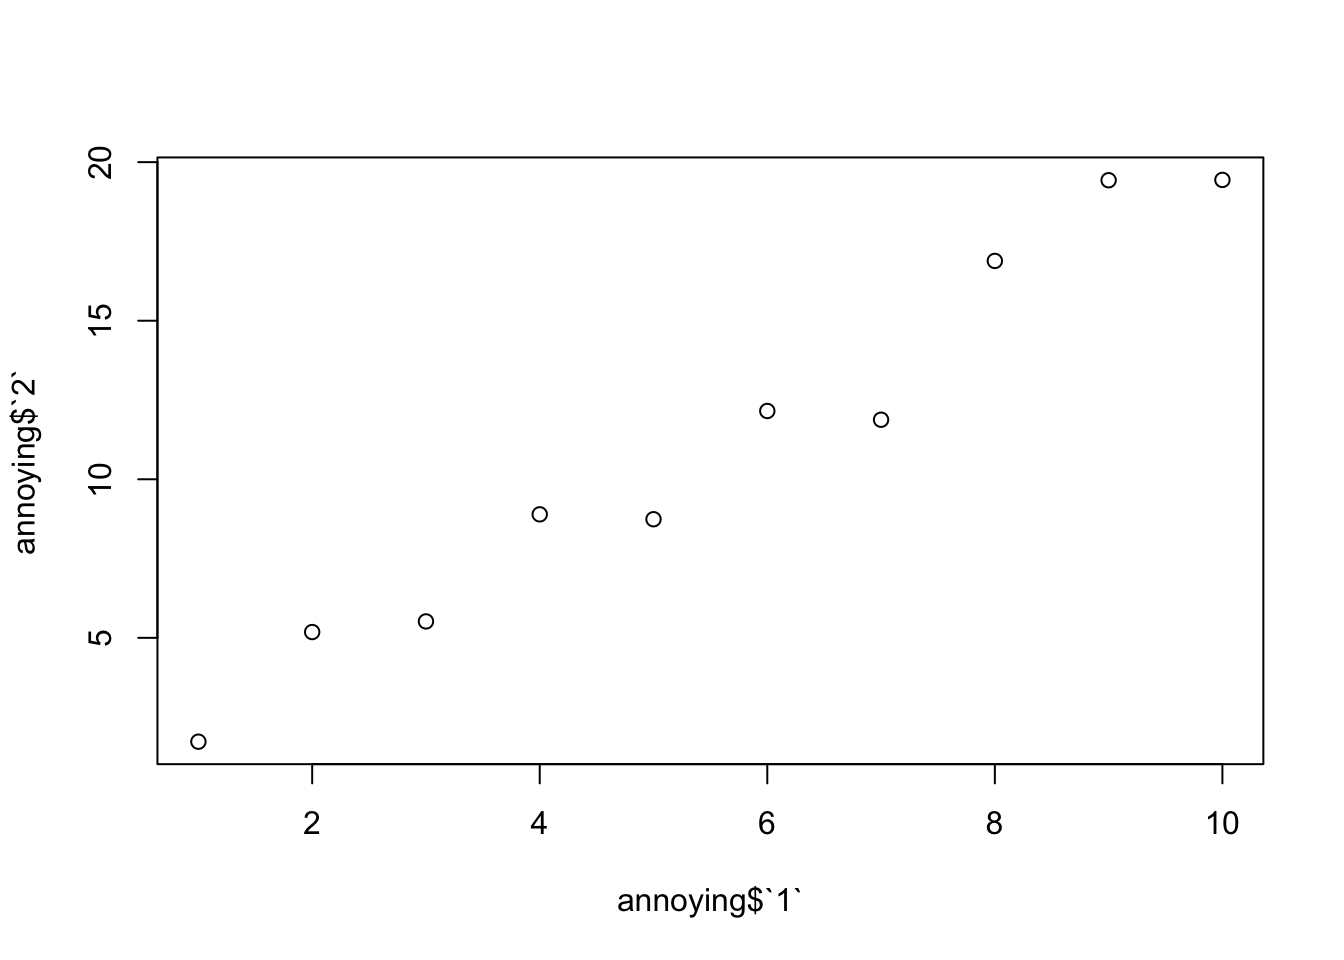
\includegraphics{bookdown-demo_files/figure-latex/unnamed-chunk-10-1.pdf}
  \item
    Use \texttt{mutate} (we haven't talked about this yet) with
    backticks

\begin{Shaded}
\begin{Highlighting}[]
\NormalTok{annoying %>%}
\StringTok{  }\KeywordTok{mutate}\NormalTok{(}\StringTok{`}\DataTypeTok{3}\StringTok{`} \NormalTok{=}\StringTok{ `}\DataTypeTok{2}\StringTok{`} \NormalTok{/}\StringTok{ `}\DataTypeTok{1}\StringTok{`}\NormalTok{)}
\end{Highlighting}
\end{Shaded}

\begin{verbatim}
## # A tibble: 10 × 3
##      `1`       `2`      `3`
##    <int>     <dbl>    <dbl>
## 1      1  1.725450 1.725450
## 2      2  5.182598 2.591299
## 3      3  5.517888 1.839296
## 4      4  8.894382 2.223596
## 5      5  8.740021 1.748004
## 6      6 12.153600 2.025600
## 7      7 11.878134 1.696876
## 8      8 16.885478 2.110685
## 9      9 19.429848 2.158872
## 10    10 19.439987 1.943999
\end{verbatim}
  \item
    Use \texttt{rename} (we haven't talked about this yet) with
    backticks

\begin{Shaded}
\begin{Highlighting}[]
\NormalTok{annoying %>%}
\StringTok{  }\KeywordTok{mutate}\NormalTok{(}\StringTok{`}\DataTypeTok{3}\StringTok{`} \NormalTok{=}\StringTok{ `}\DataTypeTok{2}\StringTok{`} \NormalTok{/}\StringTok{ `}\DataTypeTok{1}\StringTok{`}\NormalTok{) %>%}
\StringTok{  }\KeywordTok{rename}\NormalTok{(}\DataTypeTok{one =} \StringTok{`}\DataTypeTok{1}\StringTok{`}\NormalTok{, }
         \DataTypeTok{two =} \StringTok{`}\DataTypeTok{2}\StringTok{`}\NormalTok{,}
         \DataTypeTok{three =} \StringTok{`}\DataTypeTok{3}\StringTok{`}\NormalTok{)}
\end{Highlighting}
\end{Shaded}

\begin{verbatim}
## # A tibble: 10 × 3
##      one       two    three
##    <int>     <dbl>    <dbl>
## 1      1  1.725450 1.725450
## 2      2  5.182598 2.591299
## 3      3  5.517888 1.839296
## 4      4  8.894382 2.223596
## 5      5  8.740021 1.748004
## 6      6 12.153600 2.025600
## 7      7 11.878134 1.696876
## 8      8 16.885478 2.110685
## 9      9 19.429848 2.158872
## 10    10 19.439987 1.943999
\end{verbatim}
  \end{enumerate}
\item
  Look it up with \texttt{?enframe}. It turns out that
  \texttt{enframe()} is super useful.\\
  Often you will have a vector of values with names associated with it.
  For example:

\begin{Shaded}
\begin{Highlighting}[]
\NormalTok{v <-}\StringTok{ }\KeywordTok{c}\NormalTok{(}\DecValTok{1}\NormalTok{, }\DecValTok{3}\NormalTok{, }\DecValTok{4}\NormalTok{, }\DecValTok{10}\NormalTok{)}
\KeywordTok{names}\NormalTok{(v) <-}\StringTok{ }\KeywordTok{c}\NormalTok{(}\StringTok{"a"}\NormalTok{, }\StringTok{"b"}\NormalTok{, }\StringTok{"b"}\NormalTok{, }\StringTok{"c"}\NormalTok{)}
\NormalTok{v}
\end{Highlighting}
\end{Shaded}

\begin{verbatim}
##  a  b  b  c 
##  1  3  4 10
\end{verbatim}

  If you want to deal with this type of vector in the tidyverse, you can
  enframe it into a tibble:

\begin{Shaded}
\begin{Highlighting}[]
\KeywordTok{enframe}\NormalTok{(v)}
\end{Highlighting}
\end{Shaded}

\begin{verbatim}
## # A tibble: 4 × 2
##    name value
##   <chr> <dbl>
## 1     a     1
## 2     b     3
## 3     b     4
## 4     c    10
\end{verbatim}

  By default it makes columns of ``name'' and ``value''. That is
  awesome!
\item
  Do \texttt{package?tibble} and read through it to find that the answer
  we want is \texttt{tibble.max\_extra\_cols}.
\end{enumerate}

\section{Data import}\label{data-import}

\begin{itemize}
\tightlist
\item
  Why use \texttt{readr} instead of the base-R reading functions? Plenty
  of reasons.
\item
  Explicit column specifications if you want to do that.
\end{itemize}

\subsection{RStudio's GUI importer}\label{rstudios-gui-importer}

\begin{itemize}
\tightlist
\item
  This is a great way to start importing CSV files.
\item
  Don't do it every time! use the code that it creates to make reading
  your data in reproducible.
\end{itemize}

\chapter{Week Three Meeting}\label{week3}

\section{Git Basics}\label{git-basics}

Goals for Today:

\begin{itemize}
\tightlist
\item
  Explain what git is (and how it is different than GitHub)
\item
  Introduce the sha-1 hash (for fun!)
\item
  Get familiar with RStudio's very convenient interface to git

  \begin{itemize}
  \tightlist
  \item
    staging files
  \item
    unstaging file
  \item
    viewing differences between staged and unstaged files
  \item
    committing files
  \item
    viewing the commit history
  \end{itemize}
\end{itemize}

\subsection{An overview of Version Control Systems (VCS)}\label{vcs}

\begin{itemize}
\tightlist
\item
  Git is a type of VCS
\item
  At its crudest, a VCS is a system that provides a way of saving and
  restoring earlier versions of a file.
\end{itemize}

\subsubsection{A typical VCS for a non-computer
programmer}\label{a-typical-vcs-for-a-non-computer-programmer}

\begin{itemize}
\tightlist
\item
  Start writing \texttt{my\_manuscript.doc}.
\item
  At some point worry that MS Word is going to eat your file, so,

  \begin{itemize}
  \tightlist
  \item
    Make a ``backup'' called \texttt{my\_manuscript\_A.doc}
  \end{itemize}
\item
  Then, before overhauling the discussion, save the current file as
  \texttt{my\_manuscript\_B.doc}.
\item
  Email it to your coauthors and then have a series of files with other
  extensions such as the initials of their names when they edit them and
  send them back.
\item
  Etc.
\item
  Disadvantages:

  \begin{itemize}
  \tightlist
  \item
    Hard to find a good record of what is in each version. (Wait! I
    liked the introduction I wrote three weeks ago\ldots{}where is that
    now?)
  \item
    A terrible system if you have multiple files that are dependent on
    one another (for example, figures in your document, or scripts and
    data sets if you have a programming project.)
  \item
    If you decide that you want to merge the changes you made to the
    discussion in version \texttt{\_C} with the edits on the
    introduction in version \texttt{\_K}, it is hard.
  \end{itemize}
\end{itemize}

\subsubsection{Other popular VCS
systems}\label{other-popular-vcs-systems}

\begin{itemize}
\tightlist
\item
  rcs, cvs, subversion, etc.
\item
  These all had a ``Centralized'' model:

  \begin{itemize}
  \tightlist
  \item
    You set up a repository on a server that has the full version
    history,
  \item
    then each person working on it gets a copy of the current version,
    and nothing more.
  \item
    They can submit changes back to the central repository which tries
    to deal with conflicting submissions.
  \item
    You need to be online to do most operations.
  \end{itemize}
\item
  I used a few of these, and missed them for a few weeks when I switched
  to Git, but then never looked back and couldn't imagine using them
  again.
\end{itemize}

\subsubsection{The Git model --- Distributed Version
Control}\label{the-git-model-distributed-version-control}

\begin{itemize}
\tightlist
\item
  Git stores ``snapshots'' of your collection of files in a repository
\item
  For our work, the ``collection of files'' will be ``the stuff in your
  RStudio project''

  \begin{itemize}
  \tightlist
  \item
    Another reason it is nice to keep everything you need for a project
    together in a ``project directory''
  \item
    Though git scans your project directory for new additions and
    changes, it will not add a new file, or add new changes, to the
    repository until you \emph{stage} and subsequently \emph{commit} the
    file.
  \end{itemize}
\item
  When you clone a repository, \textbf{you} get the whole version
  history
\item
  When someone else clones that repository, \textbf{they also} get the
  whole version history.
\item
  Git has well-developed features for merging changes made in different
  repositories

  \begin{itemize}
  \tightlist
  \item
    But, for today, we will talk mostly of a single user interacting
    with git.
  \end{itemize}
\end{itemize}

\subsection{Git versus GitHub}\label{git-versus-github}

\begin{itemize}
\tightlist
\item
  They are not the same thing!
\item
  Git is software that you can run on your own machine for doing version
  control on a repository.

  \begin{itemize}
  \tightlist
  \item
    It can be \emph{entirely} local. i.e.~only on your hard drive and
    nowhere else.
  \item
    This is super-useful for any project, because solid version control
    is great to have.
  \end{itemize}
\item
  GitHub is a website, with tools powered by Git (and many that they
  brewed up themselves) that makes it very, very easy to share git
  repositories with people all over the place.
\end{itemize}

\subsubsection{Is everything on GitHub
public?}\label{is-everything-on-github-public}

\begin{itemize}
\tightlist
\item
  No! Many companies use GitHub to host their proprietary code

  \begin{itemize}
  \tightlist
  \item
    They just have to pay for that\ldots{}
  \end{itemize}
\item
  By default, you can put anything on GitHub for free as long as it is
  under a fairly free-use (open source type) license and it is available
  to anyone
\item
  If you want a private repository, as an academic affiliate you just
  have to ask and GitHub will give you unlimited private repos for free.
\item
  And if you are a student and you have not yet done so, go to
  \url{https://education.github.com/pack} to sign up for your free
  student pack.
\end{itemize}

\subsection{Using git through RStudio}\label{git-thru-rstudio}

\begin{itemize}
\tightlist
\item
  Now we can do a few things together to see how this works.
\item
  Most of the action is in the Git Pane\ldots{}
\item
  Today we will talk about:

  \begin{itemize}
  \tightlist
  \item
    Staging files (preparing them to be \textbf{committed})
  \item
    Committing files (putting them into the repository)
  \item
    viewing differences between staged and unstaged files
  \item
    committing files
  \item
    viewing the commit history
  \end{itemize}
\end{itemize}

\subsubsection{Two final configurations before
starting:}\label{two-final-configurations-before-starting}

\begin{itemize}
\item
  Open the shell (Tools-\textgreater{}Shell\ldots{}) and issue these two
  commands, replacing the name ``John Doe'' with yours, and his email
  with yours.

  \begin{itemize}
  \item
    You may as well use the email address that you gave to GitHub,
    though it doesn't necessarily have to be

\begin{verbatim}
git config --global user.name "John Doe"
git config --global user.email johndoe@example.com
\end{verbatim}

    You only need to do this once.
  \end{itemize}
\item
  Finally, if you are using a Mac, configure it to cache your GitHub
  credentials so you needn't give your password every time you push to
  it:

\begin{verbatim}
git config --global credential.helper osxkeychain
\end{verbatim}
\end{itemize}

\subsubsection{The status/staging panel}\label{the-statusstaging-panel}

\begin{itemize}
\tightlist
\item
  RStudio keeps git constantly scanning the project directory to find
  any files that have changed or which are new.
\item
  By clicking a file's little ``check-box'' you can stage it.\\
\item
  Some symbols:

  \begin{itemize}
  \tightlist
  \item
    \textbf{Blue-M}: a file that is already under version control that
    has been modified.
  \item
    \textbf{Yellow-?}: a file that is not under version control
    (yet\ldots{})
  \item
    \textbf{Green-A}: a file that was not under version control, but
    which has been staged to be committed.
  \item
    \textbf{Red-D}: a file under version control has been deleted. To
    make it really disappear, you have to stage its disappearance and
    commit. Note that it still lives on, but you have to dig back into
    your history to find it.
  \item
    \textbf{Purple-R} a file that was renamed. (Note that git in Rstudio
    seems to be figuring this out on its own.)
  \end{itemize}
\end{itemize}

\subsubsection{The Diff window}\label{the-diff-window}

\begin{itemize}
\tightlist
\item
  Shows what has changed between the last committed version of a file
  and its current state.
\item
  Holy smokes this is convenient
\item
  (Note: all this output is available from the command line, but the
  Rstudio interface is very nice, IMHO)
\end{itemize}

\subsubsection{Making a Commit}\label{making-a-commit}

\begin{itemize}
\tightlist
\item
  Super easy:

  \begin{itemize}
  \tightlist
  \item
    After staging the files you want to commit\ldots{}
  \item
    Write a brief message (first line short, then as much after that as
    you want) and hit the commit button.
  \end{itemize}
\end{itemize}

\subsubsection{The History window}\label{the-history-window}

\begin{itemize}
\tightlist
\item
  Easy inspection of past commits.
\item
  See what changes were made at each commit.
\end{itemize}

\subsection{Go for it everyone!}\label{git-play}

\begin{itemize}
\tightlist
\item
  Make some changes and commit them yourselves.\\
\item
  Add some new files to the project, and commit those.
\item
  Get familiar with the diff window.
\item
  Check the history after a few commits.
\end{itemize}

\subsection{How does git store and keep track of things}\label{git-how}

\begin{itemize}
\tightlist
\item
  Everything is stored in the .git folder inside the RStudio project.
\item
  The ``working copy'' gets checkout out of there
\item
  Committed changes are recorded to the directory
\end{itemize}

\subsubsection{What is inside of the .git
directory?}\label{what-is-inside-of-the-.git-directory}

We can use R to list the files. My \texttt{rep-res-course} repository
that hold all the materials for a course like this one looks like:

\begin{Shaded}
\begin{Highlighting}[]
\NormalTok{## check out this file-system command in R}
\KeywordTok{dir}\NormalTok{(}\DataTypeTok{path =} \StringTok{".git"}\NormalTok{, }\DataTypeTok{all.files =} \OtherTok{TRUE}\NormalTok{, }\DataTypeTok{recursive =} \OtherTok{TRUE}\NormalTok{)}
\end{Highlighting}
\end{Shaded}

The output from that command looks something like this:

\begin{verbatim}
  [1] "#MERGE_MSG#"                                       "COMMIT_EDITMSG"                                   
  [3] "COMMIT_EDITMSG~"                                   "config"                                           
  [5] "description"                                       "FETCH_HEAD"                                       
  [7] "HEAD"                                              "hooks/applypatch-msg.sample"                      
  [9] "hooks/commit-msg.sample"                           "hooks/post-update.sample"                         
 [11] "hooks/pre-applypatch.sample"                       "hooks/pre-commit.sample"                          
 [13] "hooks/pre-push.sample"                             "hooks/pre-rebase.sample"                          
 [15] "hooks/prepare-commit-msg.sample"                   "hooks/update.sample"                              
 [17] "index"                                             "info/exclude"                                     
 [19] "logs/HEAD"                                         "logs/refs/heads/gh-pages"                         
 [21] "logs/refs/heads/master"                            "logs/refs/remotes/origin/gh-pages"                
 [23] "logs/refs/remotes/origin/master"                   "objects/00/906f99e192ff64b4e9e9a0e5745b0a4f841cbd"
 [25] "objects/01/ab18d4ce04fb06532bb06ed579218fef89d478" "objects/02/74554e0b574b9beb2144f26ad3925830056870"
 [27] "objects/03/2d224bf78798e8b9765af6d8768ade14694a9d" "objects/04/03d552ab37b0bcaeebed0ac3068d669261c456"
 [29] "objects/04/4a12f8ccc12a4a5ba84ab2bf5a1ae751feea6f" "objects/04/9ec3065bb0434ded671fa83af5ade803bc11a1"
 [31] "objects/04/ea8efb1367727b081dea87e63818be0a4d02f0" "objects/05/b22ecc373d5058e36d7ca773a4475c46daef77"
 [33] "objects/07/8831b46c9b63e8c2d50b79304ed05de9274c28" "objects/07/b57af2a0cbd0545a6cd3e93f10cc5d768e42ba"
 [35] "objects/08/674e6e4d534b3424e2629510d20bb6d1b0be94" "objects/08/8b282d5b978dc1ff6eef3871d3fb3a9256246a"
 [37] "objects/09/565dcd10d7adc0551783b443e8fd71486b3997" "objects/09/6828a0cfb96f30d6e99cfc04a5c1686b9e318c"
 [39] "objects/0a/30fe678abc342c58daab0ad42163b371babda0" "objects/0a/b71109dae6e5711755feddfb06b81b13766496"
 [41] "objects/0b/442fdfc183783537985c17151ae3483fa00cf6" "objects/0b/c0451fd0e7081a7db05fdd38b12870bdcabd13"
 [43] "objects/0c/0f7cf8c73d901795dad4bd5f504c53c3bf2093" "objects/0d/14a7a2a19ffc3b9820f011e3270c965a5fefce"
 [45] "objects/0e/35cfb4d55e52d27083b8d2eccab9296b920d76" "objects/0e/7bba5882077a8b00a76d3eabe6b23cadc658e6"
 [47] "objects/0e/8abf4cc0885a727ee2459fdbb272828e267cc4" "objects/0f/1f3f7be7787d5d44dc1155f3b7a44eddc9f0be"
 [49] "objects/10/54d2e7a9baf61618521c522b15db40855b3431" "objects/11/7d874e1616500b5fba51b9f0ee1e8d0fbe1dc2"
 [51] "objects/11/c33cc1d5c8de7c7cbf7257b7d32f7ca3d458ef" "objects/14/1ccea514e106e20eef47b791a23e036d1fa1d2"
 [53] "objects/15/cc3a6f15dadb3446ad0af34a3ecde8d81d65f9" "objects/15/ddaf45bf00c3ef2d8f499ebd6dc3a86bf9c3ab"
 [55] "objects/16/0c9386dfa9707d81fbbbcc52f0c7638703f9a9" "objects/16/8ee93b6a4612dbd76bc06a49460df9f9f6c41b"
\end{verbatim}

\textbf{Yikes!}

\subsubsection{How does git know a file has
changed?}\label{how-does-git-know-a-file-has-changed}

\begin{itemize}
\tightlist
\item
  Does it just look at the modification date?
\item
  NO! It ``fingerprints'' every file, so it knows when it has changed
  from the most recent committed version.

  \begin{itemize}
  \tightlist
  \item
    Demonstration. Change a file. Save, then undo the change and save
    again\ldots{}Git knows the file has been changed back to its
    ``former self''
  \end{itemize}
\item
  SHA-1 hashes. We will learn more about those later.\\
\item
  You will see things like
  \texttt{ed00c10ae6cf7bcc35d335d2edad7e71bc0f6770} all over in
  Git-land.
\item
  You can treat them as very specific names for different commits.
\end{itemize}

\subsubsection{What should I keep under version
control?}\label{what-should-i-keep-under-version-control}

\begin{itemize}
\tightlist
\item
  General rule: don't keep derived products.

  \begin{itemize}
  \tightlist
  \item
    i.e.~If you have an Rmd file that creates an html file, there isn't
    much need to put the html file under version control with git,
    because you can just regenerate it by Knitting the Rmd file.
  \end{itemize}
\item
  Do keep data, source code, etc.
\item
  Sometimes certain outputs and intermediate results from long
  calculations can be committed so that you don't have to run a 4 hour
  analysis to start where you were before.
\item
  For such results, consider \texttt{saveRDS()} with the
  \texttt{compress\ =\ "xz"} option (and its companion
  \texttt{readRDS()}.
\end{itemize}

\subsubsection{How can I make git ignore certain
files?}\label{how-can-i-make-git-ignore-certain-files}

\begin{itemize}
\tightlist
\item
  The \texttt{.gitignore} file!
\item
  File names (and patterns) in the \texttt{.gitignore} file are ignored
  \emph{recursively} (down into subdirectories), by default.
\item
  Files won't be ignored if they are already in the repository.
\item
  Example: \texttt{*.html}
\end{itemize}

\section{Pushing and Pulling With
GitHub}\label{pushing-and-pulling-with-github}

\subsection{Creating a Repository on GitHub and the initial
push}\label{creating-a-repository-on-github-and-the-initial-push}

When you have an RStudio project under git version control on your
laptop or desktop computer, creating a remote repository on GitHub is
quite easy. A few steps:

\begin{enumerate}
\def\labelenumi{\arabic{enumi}.}
\tightlist
\item
  Upper right corner: ``create new'' button (a ``+'' with a little
  triangle.) Choose ``New Repository''
\item
  Give it a name. It makes most sense to name it the same as the RStudio
  project you want to push up there. So, for example, if my project file
  was \texttt{boing.Rproj}, I would name the repository \texttt{boing}.
\item
  Add a 5 or 6 word description if you want.
\item
  Choose \textbf{public} or \textbf{private}
\item
  DO \textbf{NOT} choose to ``Initialize this repository with a
  README''. You likely already have a README. Initializing the
  repository with one will create headaches.
\item
  Also, don't add a \texttt{.gitignore} or a license (select ``none'',
  which should be the default, for both of those)
\item
  Click the green ``Create Repository'' button
\end{enumerate}

That will take you to another screen. In the middle find the code box
below the heading, \textbf{\ldots{}or push an existing repository from
the command line}.

\begin{enumerate}
\def\labelenumi{\arabic{enumi}.}
\item
  Copy that two lines of code from you web browser. It will look
  something like this:

\begin{verbatim}
git remote add origin https://github.com/eriqande/boing.git
git push -u origin master
\end{verbatim}

  but it will be specific to the repository you just made, so the URL
  and name of the repo will be different than what you see above. Note,
  you can copy the lines by clicking the ``copy this text'' icon on the
  right side of the page.
\item
  Go to RStudio, in the project that you want to push to GitHub, and
  choose ``Tools-Shell''. That will give you a terminal window. Paste
  the commands you copied into that terminal window and hit return.
\item
  It might ask you for your GitHub username and password.
\end{enumerate}

Voila!

\subsection{Subsequent pushes}\label{subsequent-pushes}

Once you have pushed the repo up there. Try making some changes on your
laptop, committing them, and then hitting the ``Push'' button on the git
panel\ldots{}

\subsection{Assign collaborators}\label{assign-collaborators}

From the repository page on GitHub, choose ``Settings'' (on the upper
right) and find the ``collaborators'' link (on the left).

If you have a private repository, you can add GitHub user
\texttt{eriqande} (that's me\ldots{}) to it and I will be able to view
it and give comments and suggestions.

\section{Next Week's Assignment}\label{next-weeks-assignment}

\begin{itemize}
\tightlist
\item
  With luck, we will get everyone's projects up to GitHub before the end
  of our session today. However, if we don't, please get that done ASAP.
\item
  The big assignment is to read the
  \href{http://r4ds.had.co.nz/transform.html}{Data Transformation}
  chapter in ``R for Data Science.'' \emph{Warning}: This is a long and
  meaty chapter, so get an early start! The chapter goes through what
  you need to know to leverage all the \texttt{dplyr} goodness. Please
  work all the examples, and do the exercises. In fact, when you are
  working through the examples with the \texttt{nycflights} data set,
  you should, after each example, try to do the same type of operation
  on your own data set.
\end{itemize}

\chapter{Week Four Meeting}\label{week4}

This was a bit of a free-form discussion on a variety of topics.

\section{Knit your README.Rmd files}\label{knit-your-readme.rmd-files}

First thing we talked about was the fact that GitHub will render a
\texttt{README.md} file to an html web page that is nice and easy to
read. It will sort of render a README.Rmd file, but it won't do
everything to it. Namely:

\begin{enumerate}
\def\labelenumi{\arabic{enumi}.}
\tightlist
\item
  The YAML header block comes out as a table.
\item
  It will \textbf{not} evaluate all the R code and deliver the results.
\end{enumerate}

Rather, it is necessary to locally \emph{knit} the \texttt{README.Rmd}
file to create a \texttt{README.md}, then this \texttt{README.md} file
must be committed to the repository and pushed. This needs to happen
each time you have updated the \texttt{README.Rmd} file.

Note that your \texttt{README.Rmd} file should start with the following:

\begin{Shaded}
\begin{Highlighting}[]
\KeywordTok{cat}\NormalTok{(}\KeywordTok{readLines}\NormalTok{(}\StringTok{"inputs/readme-header.txt"}\NormalTok{), }\DataTypeTok{sep =} \StringTok{'}\CharTok{\textbackslash{}n}\StringTok{'}\NormalTok{)}
\end{Highlighting}
\end{Shaded}

\begin{verbatim}
---
title: "NameOfPackage"
date: "`r format(Sys.time(), '%d %B, %Y')`"
output: 
  github_document:
    toc: true
---

<!-- README.md is generated from README.Rmd. Please edit that file -->

```{r, echo = FALSE}
knitr::opts_chunk$set(
  collapse = TRUE,
  comment = "#>",
  fig.path = "readme-figs/"
)
```

Then start adding your text here...
\end{verbatim}

\section{Changing to factors}\label{changing-to-factors}

Mikki had a question: she wanted to have a column that contained 1's and
2's as factors. her data set had several entries that were ``1,2''. She
wanted to convert those to 2's and then make them all factors. We
discussed how this could be done with dplyr. The important message was
that dplyr does not change the original input variable, but in the
output, you can ``mutate over the top of an existing variable'' (i.e.~in
the output the column will have been changed, but not in the original
input data frame).

\section{\texorpdfstring{The \texttt{group\_by()}
function}{The group\_by() function}}\label{the-group_by-function}

We spent a bit of time going over how to think about what the
\texttt{group\_by()} function does. Eric likes to think of it as
breaking your original tibble up into a lot of different tibbles,
according to the grouping variables, after which, each little tibble
gets sent to the following verb (\texttt{summarise()},
\texttt{mutate()}, \texttt{filter()}, etc.)

We talked about that fact that while it is quite natural to think about
using the \texttt{group\_by()} function in conjunction with
\texttt{summarise()}, it is also very powerful to be able to use it in
conjuntion with \texttt{mutate()}.

When you do a summarise, only the grouping variables and the
newly-created summary variables get returned in the output tibble, and
the rows are arranged by the grouping variables. When you do a
\texttt{group\_by()} and then \texttt{mutate()} all of the columns get
returned and there is no automatic arranging that goes on.

\section{\texorpdfstring{How do I learn about all the vectorized
functions I can use in \texttt{mutate()} and
\texttt{summarize()}?}{How do I learn about all the vectorized functions I can use in mutate() and summarize()?}}\label{how-do-i-learn-about-all-the-vectorized-functions-i-can-use-in-mutate-and-summarize}

There was consensus in the class that even once we have learned the
mechanics of using \texttt{mutate()} and \texttt{summarise()}, we might
still be at a loss as to \emph{how} to use them, or with which
functions. Admittedly, there are many, many vectorized functions in R
that you might apply within a \texttt{mutate()} or \texttt{summarise()}
function, and learning about all of those, and having them at your
fingertips when you need them is part of the never-ending journey of
gaining experience with R.

However, there are a few things that can help with that journey. Here
are my two favorite suggestions:

\begin{enumerate}
\def\labelenumi{\arabic{enumi}.}
\tightlist
\item
  Get the RStudio \emph{dplyr cheatsheet}. In RStudio, Go to
  Help--\textgreater{}Cheatsheets--\textgreater{}Data
  Manipulation-with-dplyr,-tidyr. While you are at it. Check out their
  other cheatsheets.
\item
  Review Hadley's Advanced R
  \href{http://adv-r.had.co.nz/Vocabulary.html}{recommended
  vocabulary}.\\
  This is a nice, compact list of R functions that you should be
  familiar with, or at least aware of.
\end{enumerate}

\section{Next Week's Assignment}\label{next-weeks-assignment-1}

For Week 5, we are going to talk about \textbf{joins}. This is a very
important topic for combining data from different data sets. Thus,
everyone should read
\href{http://r4ds.had.co.nz/relational-data.html}{Chapter 13: Relational
Data} in the R for Data Science Book. This is an amazing chapter, and
will go a long way in helping people understand how to make their lives
easier when it comes to combining multiple tibbles of information (for
example, a tibble of metadata for each individual and a tibble of
genotype information, for the same individauls, etc.). Try to work
through all the examples and do the exercises.

\chapter{Week Five Meeting}\label{week5}

\section{Some things regarding people's
repositories}\label{some-things-regarding-peoples-repositories}

\subsection{Data Compression}\label{data-compression}

We have been endorsing \texttt{.csv} as a good format for data, and
\emph{it is}, because it is human-readable and easily parsed into
tibbles. However, when you have very long tibbles, it is not necessarily
the most space-efficient format. Large \texttt{.csv} files can take up
much more space on your hard drive \emph{than they should}.

What do we mean by ``\emph{than they should?}'' in that context? This
has to do with how much \emph{information} is in the file, where
information is used in the context of \emph{information theory}. Often
tibbles will have columns that have fairly ``redundant''
information---for example, in a mutlispecies salmon data set, one column
might have entries that are either ``Chinook'', ``coho'', or
``steelhead''. It takes a few bytes to store each one of those words,
and if they are used in a column that has millions of rows, that can add
up to a lot of space on your hard drive. Colloquially, \emph{data
compression} is the art of finding ways of using short ``code-names''
for things or patterns that occur frequently in a file, and in so doing,
reducing the overall file size.

The consequences of data compression can be profound and wonderful. You
can reduce the size of a file, sometimes by an order or magnitude or
more. There are a few good choices available for compressing your data
(making it smaller.). Note that doing so often makes it a little harder
to edit your data set; however, if your data set is not going to change,
and it is large, then it makes sense to compress it---especially if it
is so big you would rather not (or can't) put it on GitHub.

\subsubsection{gzip}\label{gzip}

If you are working on a Mac, you have the Unix utility \texttt{gzip}. We
will illustrate its use on Katie's big salmon data set,
\texttt{ASL\_merged.csv}. Let's see how big that is. We can use the Unix
utility \texttt{du} (stands for ``disk usage'').

\begin{Shaded}
\begin{Highlighting}[]
\CommentTok{# give this command on the Terminal in the directory where the file lives:}
\KeywordTok{du} \NormalTok{-h ASL_merged.csv }
\end{Highlighting}
\end{Shaded}

The results comes back:

\begin{verbatim}
322M    ASL_merged.csv
\end{verbatim}

Whoa! This file is 332 Megabytes. That is quite large!

However, we can compress it like this:

\begin{Shaded}
\begin{Highlighting}[]
\KeywordTok{gzip} \NormalTok{ASL_merged.csv }
\end{Highlighting}
\end{Shaded}

When we do that, it compresses the file and renames it to have a
\texttt{.gz} extension on it: \texttt{ASL\_merged.csv.gz}. We can then
see how big that file is:

\begin{Shaded}
\begin{Highlighting}[]
\KeywordTok{du} \NormalTok{-h ASL_merged.csv.gz }
\end{Highlighting}
\end{Shaded}

tells us:

\begin{verbatim}
11M ASL_merged.csv.gz
\end{verbatim}

Whoa! We went from 332 Megabytes to 11. It is just 3\% of its original
size (and small enough that you can safely put it on GitHub).

One very nice feature is that gzipped files can be read in directly by
the functions of the \texttt{readr} package. So, for example,
\texttt{read\_csv()} works just fine on the gzipped version of Katie's
massive salmon data set:

\begin{Shaded}
\begin{Highlighting}[]
\CommentTok{# this works the same as it would on the ungzipped file}
\NormalTok{salmon <-}\StringTok{ }\KeywordTok{read_csv}\NormalTok{(}\StringTok{"data/ASL_merged.csv.gz"}\NormalTok{)}
\end{Highlighting}
\end{Shaded}

\subsubsection{\texorpdfstring{\texttt{xz} comression with
\texttt{saveRDS()}}{xz comression with saveRDS()}}\label{xz-comression-with-saverds}

Another method that can be even more efficient with tibbles is to store
them as R objects using the \texttt{saveRDS()} function with the
\texttt{xz} compression option. This has the nice advantage that all the
data types of the variables (for example, if you had made factors out of
some) will be preserved \emph{exactly} as they are in the tibble when
you save it.

Let's imagine we have read the tibble into the variable \texttt{salmon},
and all the column types were as we wanted. Then, we could save that
tibble directly to a compressed file like this:

\begin{Shaded}
\begin{Highlighting}[]
\KeywordTok{saveRDS}\NormalTok{(salmon, }\DataTypeTok{file =} \StringTok{"ASL_xz.rds"}\NormalTok{, }\DataTypeTok{compress =} \StringTok{"xz"}\NormalTok{)}
\end{Highlighting}
\end{Shaded}

Note that \texttt{compress\ =\ "xz"} option. Let's see how that did
using \texttt{du} on the Unix terminal:

\begin{Shaded}
\begin{Highlighting}[]
\KeywordTok{du} \NormalTok{-h ASL_xz.rds}
\end{Highlighting}
\end{Shaded}

tells us:

\begin{verbatim}
3.7M    ASL_xz.rds
\end{verbatim}

Holy Smokes! Only 3.7 Megabytes. That is only 1.1\% of its original
size. Lovely!

In order to read that tibble back into a variable (named
\texttt{my\_var}, say) in R, you would use \texttt{readRDS()} like this:

\begin{Shaded}
\begin{Highlighting}[]
\NormalTok{my_var <-}\StringTok{ }\KeywordTok{readRDS}\NormalTok{(}\DataTypeTok{file =} \StringTok{"ASL_xz.rds"}\NormalTok{)}
\end{Highlighting}
\end{Shaded}

Voila!

\section{A quick aside about missing
data}\label{a-quick-aside-about-missing-data}

Garrett and Hadley note that ``missing values are `contagious': almost
any operation involving an unknown value will also be unknown.'' This is
true for the most part, but there is a vexing inconsistency. Observe

This gives us NA as we would hope it would

\begin{Shaded}
\begin{Highlighting}[]
\OtherTok{NA} \NormalTok{==}\StringTok{ }\DecValTok{0} \NormalTok{|}\StringTok{ }\OtherTok{NA} \NormalTok{==}\StringTok{ }\DecValTok{1}
\end{Highlighting}
\end{Shaded}

\begin{verbatim}
## [1] NA
\end{verbatim}

However, this one returns FALSE. What gives?

\begin{Shaded}
\begin{Highlighting}[]
\OtherTok{NA} \NormalTok\StringTok{ }\KeywordTok{c}\NormalTok{(}\DecValTok{0}\NormalTok{, }\DecValTok{1}\NormalTok{)}
\end{Highlighting}
\end{Shaded}

\begin{verbatim}
## [1] FALSE
\end{verbatim}

\section{Brief Highlights of the Joins
Chapter}\label{brief-highlights-of-the-joins-chapter}

You will likely end up using joins all the time. As noted in the book,
the \texttt{left\_join()} is what you will likely use all the time. In
this case you have a ``focal'' data frame with all the rows (``cases''
or ``observations'') in the \texttt{x} table that you are going to be
wanting to add some columns to. Those columns live in the \texttt{y}
table (along with the matching keys).

``\emph{The left join should be your default join: use it unless you
have a strong reason to prefer one of the others.}''

You an do the same things with base R's \texttt{merge()} function, but
it is slower and somewhat harder to express your intent with it. (I've
always really disliked the \texttt{merge()} function\ldots{})

\subsection{A few thoughts on keys}\label{a-few-thoughts-on-keys}

It is always a worthwhile exercise to go through and figure out what the
\emph{primary key} is in a tibble you are working with. It might be that
the primary key is a compound key: it defines unique observations by a
combination of several variables. Sometimes there is no explicit primary
key! It is worthwhile to add a \emph{surrogate key} in that case.

On the flip side of these issues: when you are compiling your own data
set, you might want to spend some time making sure that units that might
be relevant to an analysis are explicitly identified in a single column.
Here is an example: the NOAA Observer program takes tissue samples from
bycatch for genetic analysis. There is a primary key
\texttt{tissue\_sample} for every tissue sample. However, under some
circumstances they take multiple tissue samples from the same
individual. But they don't have a column in the data set with an
indvividual ID. So, when the send their samples to people who will
genotype them, a lot of individuals are unwittingly genotyped twice.
Their response: ``Well, isn't it obvious that if a tissue sample is
taken from a fish that was caught on the same \texttt{vessel} on the
same \texttt{day} and in the same \texttt{haul}, and is of the same
\texttt{species} and has the same recorded \texttt{length} is the same
individual?'' My response: ``\textbf{NO! It isn't!}. Don't make people
use a whole lot of columns to identify things that should be identified
in a single column!''

\section{An example of using some
joins}\label{an-example-of-using-some-joins}

Let's walk through a simple case that should be familiar to those in the
group who have worked with genetic data and have had to deal with the
problem of attaching meta data to genetic data coming off a genotyping
instrument.

Typically those data come out in a form that can be made into a tibble.
Let's read in a toy example:

\begin{Shaded}
\begin{Highlighting}[]
\KeywordTok{library}\NormalTok{(tidyverse)}
\NormalTok{genos <-}\StringTok{ }\KeywordTok{read_csv}\NormalTok{(}\StringTok{"inputs/toy_geno.csv"}\NormalTok{)}
\NormalTok{genos}
\end{Highlighting}
\end{Shaded}

\begin{verbatim}
## # A tibble: 8 × 5
##     bird locus1_a locus1_b locus2_a locus2_b
##    <chr>    <int>    <int>    <int>    <int>
## 1 wiwa01        1        2        3        3
## 2 wiwa02        2        2        4        4
## 3 wiwa03        2        2        3        4
## 4 wiwa04        1        1        4        4
## 5 wiwa05        2        2        3        4
## 6 wiwa06        1        1        4        4
## 7 wiwa07        1        2        3        4
## 8 wiwa08        1        1        3        4
\end{verbatim}

There is a single column (\texttt{bird} in this case) that is the
primary key that uniquely identifies individuals. Then each locus gets
two columns of data (one for each gene copy in a diploid).

That is all well and good. But now, consider this problem: for a
particular analysis we are going to do, we need to have the latitude and
longitude coordinates where each bird was sampled. Let's say that we got
these samples from friendly collectors who provided a meta data file
that gave us the collection location and the name of the collector.
Let's look at that:

\begin{Shaded}
\begin{Highlighting}[]
\NormalTok{meta <-}\StringTok{ }\KeywordTok{read_csv}\NormalTok{(}\StringTok{"inputs/toy_meta.csv"}\NormalTok{)}
\NormalTok{meta}
\end{Highlighting}
\end{Shaded}

\begin{verbatim}
## # A tibble: 10 × 3
##    field_id location collector
##       <chr>    <chr>     <chr>
## 1    wiwa01     swAZ       joe
## 2    wiwa02     nwAZ      mary
## 3    wiwa03     soCA       ted
## 4    wiwa05     soCA       ted
## 5    wiwa06     swAZ       joe
## 6    wiwa08     noCA      erin
## 7    wiwa09     noCA      erin
## 8    wiwa10     noCA      erin
## 9    wiwa11     noCA      erin
## 10   wiwa12     noCA      erin
\end{verbatim}

\textbf{Notice:} there are some birds in this data set that we don't
have in the \texttt{genos} tibble. Not only that, but if you look
closely, it is missing some birds in \texttt{genos}: they are ``wiwa04''
and ``wiwa07''. Also, note that the column that holds the ID of each
bird is called \texttt{field\_id} not \texttt{bird}.

Finally, the network of bird sample collectors maintains a data base of
all their location codes that looks like this:

\begin{Shaded}
\begin{Highlighting}[]
\NormalTok{locations <-}\StringTok{ }\KeywordTok{read_csv}\NormalTok{(}\StringTok{"inputs/toy_locations.csv"}\NormalTok{)}
\NormalTok{locations}
\end{Highlighting}
\end{Shaded}

\begin{verbatim}
## # A tibble: 6 × 3
##   location   lat   long
##      <chr> <dbl>  <dbl>
## 1     swAZ  32.1 -112.8
## 2     nwAZ  36.8 -113.5
## 3     soCA  33.2 -117.1
## 4     noCA  40.6 -123.9
## 5     soOR  42.9 -123.7
## 6     noOR  45.9 -123.1
\end{verbatim}

Aha! So, what we need to do is associate with each \texttt{bird} a
\texttt{location}, and then once we have done with that, we need to
associate a \texttt{lat} and a \texttt{long} with those locations. This
is the perfect job for a join (two of them, actually).

Note that we are focused on our birds, here, so we want to keep them all
around and not add any information where we don't have a bird. Hence
\texttt{left\_join()} is our go-to friend there (as it almost always
will be).

Here is what the first step looks like:

\begin{Shaded}
\begin{Highlighting}[]
\NormalTok{genos %>%}
\StringTok{  }\KeywordTok{left_join}\NormalTok{(., meta, }\DataTypeTok{by =} \KeywordTok{c}\NormalTok{(}\StringTok{"bird"} \NormalTok{=}\StringTok{ "field_id"}\NormalTok{))}
\end{Highlighting}
\end{Shaded}

\begin{verbatim}
## # A tibble: 8 × 7
##     bird locus1_a locus1_b locus2_a locus2_b location collector
##    <chr>    <int>    <int>    <int>    <int>    <chr>     <chr>
## 1 wiwa01        1        2        3        3     swAZ       joe
## 2 wiwa02        2        2        4        4     nwAZ      mary
## 3 wiwa03        2        2        3        4     soCA       ted
## 4 wiwa04        1        1        4        4     <NA>      <NA>
## 5 wiwa05        2        2        3        4     soCA       ted
## 6 wiwa06        1        1        4        4     swAZ       joe
## 7 wiwa07        1        2        3        4     <NA>      <NA>
## 8 wiwa08        1        1        3        4     noCA      erin
\end{verbatim}

Notice that we have some NAs for birds that are not in the meta data.
That is the behavior we expect from \texttt{left\_join()}: it is not
going to discard some of your birds, just because they don't appear in
the meta data.

Note also that when we explicitly give the names of the keys (which
differ in the different tibbles) the one on the left corresponds to the
\texttt{x} argument to \texttt{left\_join()}. Also, notice that these
key names \emph{must be quoted}!! (It is easy to forget that, because
you so seldom need quotation marks around things in the tidyverse.)

Now, we can add the lat-longs on there. We will show how that is done by
chaining onto the previous command:

\begin{Shaded}
\begin{Highlighting}[]
\NormalTok{genos %>%}
\StringTok{  }\KeywordTok{left_join}\NormalTok{(., meta, }\DataTypeTok{by =} \KeywordTok{c}\NormalTok{(}\StringTok{"bird"} \NormalTok{=}\StringTok{ "field_id"}\NormalTok{)) %>%}
\StringTok{  }\KeywordTok{left_join}\NormalTok{(., locations)}
\end{Highlighting}
\end{Shaded}

\begin{verbatim}
## Joining, by = "location"
\end{verbatim}

\begin{verbatim}
## # A tibble: 8 × 9
##     bird locus1_a locus1_b locus2_a locus2_b location collector   lat
##    <chr>    <int>    <int>    <int>    <int>    <chr>     <chr> <dbl>
## 1 wiwa01        1        2        3        3     swAZ       joe  32.1
## 2 wiwa02        2        2        4        4     nwAZ      mary  36.8
## 3 wiwa03        2        2        3        4     soCA       ted  33.2
## 4 wiwa04        1        1        4        4     <NA>      <NA>    NA
## 5 wiwa05        2        2        3        4     soCA       ted  33.2
## 6 wiwa06        1        1        4        4     swAZ       joe  32.1
## 7 wiwa07        1        2        3        4     <NA>      <NA>    NA
## 8 wiwa08        1        1        3        4     noCA      erin  40.6
## # ... with 1 more variables: long <dbl>
\end{verbatim}

Voila! That is what we wanted. Now, we could filter out those NAs and
drop the \texttt{collector} column, if desired.

Notice that, since the \texttt{location} column was named
\texttt{location} in tibble, \texttt{left\_join()} just used that.

\subsection{\texorpdfstring{When would I use
\texttt{right\_join()}?}{When would I use right\_join()?}}\label{when-would-i-use-right_join}

The only time I use this is when I want to add columns to the beginning
of a tibble, but I want to preserve all the keys in the table that is
going to end up with its columns on the right hand side of the table.
And even then I usually just use \texttt{select} after a
\texttt{left\_join()}. Perhaps an example will be best: for some
purposes it is best to keep the genotype data all together on the right
hand side of the tibble (often genotype data can take up lots of columns
and you might want to be able to see the columns you have joined on
without using View() and scrolling way over). In this case you can do
this:

\begin{Shaded}
\begin{Highlighting}[]
\NormalTok{genos %>%}
\StringTok{  }\KeywordTok{right_join}\NormalTok{(meta, ., }\DataTypeTok{by =} \KeywordTok{c}\NormalTok{(}\StringTok{"field_id"} \NormalTok{=}\StringTok{ "bird"}\NormalTok{)) %>%}
\StringTok{  }\KeywordTok{right_join}\NormalTok{(locations, .) }
\end{Highlighting}
\end{Shaded}

\begin{verbatim}
## Joining, by = "location"
\end{verbatim}

\begin{verbatim}
## # A tibble: 8 × 9
##   location   lat   long field_id collector locus1_a locus1_b locus2_a
##      <chr> <dbl>  <dbl>    <chr>     <chr>    <int>    <int>    <int>
## 1     swAZ  32.1 -112.8   wiwa01       joe        1        2        3
## 2     nwAZ  36.8 -113.5   wiwa02      mary        2        2        4
## 3     soCA  33.2 -117.1   wiwa03       ted        2        2        3
## 4     <NA>    NA     NA   wiwa04      <NA>        1        1        4
## 5     soCA  33.2 -117.1   wiwa05       ted        2        2        3
## 6     swAZ  32.1 -112.8   wiwa06       joe        1        1        4
## 7     <NA>    NA     NA   wiwa07      <NA>        1        2        3
## 8     noCA  40.6 -123.9   wiwa08      erin        1        1        3
## # ... with 1 more variables: locus2_b <int>
\end{verbatim}

Notice that when you do this, the column name of the \texttt{x}
variable, \texttt{field\_id} is the one that gets retained.

\subsection{\texorpdfstring{What about that
\texttt{inner\_join()}}{What about that inner\_join()}}\label{what-about-that-inner_join}

If you knew ahead of time that you couldn't use any birds that you
didn't have lat-longs for, you could start with an
\texttt{inner\_join()}, because that would discard birds that don't have
an entry in the meta data:

\begin{Shaded}
\begin{Highlighting}[]
\NormalTok{genos %>%}
\StringTok{  }\KeywordTok{inner_join}\NormalTok{(., meta, }\DataTypeTok{by =} \KeywordTok{c}\NormalTok{(}\StringTok{"bird"} \NormalTok{=}\StringTok{ "field_id"}\NormalTok{))}
\end{Highlighting}
\end{Shaded}

\begin{verbatim}
## # A tibble: 6 × 7
##     bird locus1_a locus1_b locus2_a locus2_b location collector
##    <chr>    <int>    <int>    <int>    <int>    <chr>     <chr>
## 1 wiwa01        1        2        3        3     swAZ       joe
## 2 wiwa02        2        2        4        4     nwAZ      mary
## 3 wiwa03        2        2        3        4     soCA       ted
## 4 wiwa05        2        2        3        4     soCA       ted
## 5 wiwa06        1        1        4        4     swAZ       joe
## 6 wiwa08        1        1        3        4     noCA      erin
\end{verbatim}

But, it will probably be easier to follow if you \emph{explicitly
discard those birds} using \texttt{filter()} or by doing a filtering
join.

\subsection{An anti\_join example}\label{an-anti_join-example}

If you want to get all the genotype data for birds that don't occur in
the meta data you can use the filtering \texttt{anti\_join()}:

\begin{Shaded}
\begin{Highlighting}[]
\NormalTok{genos %>%}
\StringTok{  }\KeywordTok{anti_join}\NormalTok{(., meta, }\DataTypeTok{by =} \KeywordTok{c}\NormalTok{(}\StringTok{"bird"} \NormalTok{=}\StringTok{ "field_id"}\NormalTok{))}
\end{Highlighting}
\end{Shaded}

\begin{verbatim}
## # A tibble: 2 × 5
##     bird locus1_a locus1_b locus2_a locus2_b
##    <chr>    <int>    <int>    <int>    <int>
## 1 wiwa07        1        2        3        4
## 2 wiwa04        1        1        4        4
\end{verbatim}

And to return only those rows for birds that are in the meta data, you
could use \texttt{semi\_join()}:

\begin{Shaded}
\begin{Highlighting}[]
\NormalTok{genos %>%}
\StringTok{  }\KeywordTok{semi_join}\NormalTok{(., meta, }\DataTypeTok{by =} \KeywordTok{c}\NormalTok{(}\StringTok{"bird"} \NormalTok{=}\StringTok{ "field_id"}\NormalTok{))}
\end{Highlighting}
\end{Shaded}

\begin{verbatim}
## # A tibble: 6 × 5
##     bird locus1_a locus1_b locus2_a locus2_b
##    <chr>    <int>    <int>    <int>    <int>
## 1 wiwa01        1        2        3        3
## 2 wiwa02        2        2        4        4
## 3 wiwa03        2        2        3        4
## 4 wiwa05        2        2        3        4
## 5 wiwa06        1        1        4        4
## 6 wiwa08        1        1        3        4
\end{verbatim}

Note that we could turn it around in order to see which birds are in the
meta data, but which don't occur in the genos:

\begin{Shaded}
\begin{Highlighting}[]
\NormalTok{genos %>%}
\StringTok{  }\KeywordTok{anti_join}\NormalTok{(meta, ., }\DataTypeTok{by =} \KeywordTok{c}\NormalTok{(}\StringTok{"field_id"} \NormalTok{=}\StringTok{ "bird"}\NormalTok{))}
\end{Highlighting}
\end{Shaded}

\begin{verbatim}
## # A tibble: 4 × 3
##   field_id location collector
##      <chr>    <chr>     <chr>
## 1   wiwa12     noCA      erin
## 2   wiwa11     noCA      erin
## 3   wiwa10     noCA      erin
## 4   wiwa09     noCA      erin
\end{verbatim}

Dammit Erin! You always forget to send us the friggin' samples! Clearly
smokin' too much of the kind green there in noCA. (Note. These names
really are totally fictitious.)

Quick quiz: why would this not work:

\begin{Shaded}
\begin{Highlighting}[]
\NormalTok{genos %>%}
\StringTok{   }\KeywordTok{anti_join}\NormalTok{(meta, ., }\DataTypeTok{by =} \KeywordTok{c}\NormalTok{(}\StringTok{"bird"} \NormalTok{=}\StringTok{ "field_id"}\NormalTok{))}
\end{Highlighting}
\end{Shaded}

\subsection{Just for fun, let's see a
full\_join()}\label{just-for-fun-lets-see-a-full_join}

This bad boy makes a row with NAs for values in \emph{either} tibble
that are not matched in the other:

\begin{Shaded}
\begin{Highlighting}[]
\NormalTok{genos %>%}
\StringTok{  }\KeywordTok{full_join}\NormalTok{(., meta, }\DataTypeTok{by =} \KeywordTok{c}\NormalTok{(}\StringTok{"bird"} \NormalTok{=}\StringTok{ "field_id"}\NormalTok{)) %>%}
\StringTok{  }\KeywordTok{full_join}\NormalTok{(., locations) %>%}
\StringTok{  }\KeywordTok{print}\NormalTok{(}\DataTypeTok{n =} \DecValTok{20}\NormalTok{) }\CommentTok{# so all rows print}
\end{Highlighting}
\end{Shaded}

\begin{verbatim}
## Joining, by = "location"
\end{verbatim}

\begin{verbatim}
## # A tibble: 14 × 9
##      bird locus1_a locus1_b locus2_a locus2_b location collector   lat
##     <chr>    <int>    <int>    <int>    <int>    <chr>     <chr> <dbl>
## 1  wiwa01        1        2        3        3     swAZ       joe  32.1
## 2  wiwa02        2        2        4        4     nwAZ      mary  36.8
## 3  wiwa03        2        2        3        4     soCA       ted  33.2
## 4  wiwa04        1        1        4        4     <NA>      <NA>    NA
## 5  wiwa05        2        2        3        4     soCA       ted  33.2
## 6  wiwa06        1        1        4        4     swAZ       joe  32.1
## 7  wiwa07        1        2        3        4     <NA>      <NA>    NA
## 8  wiwa08        1        1        3        4     noCA      erin  40.6
## 9  wiwa09       NA       NA       NA       NA     noCA      erin  40.6
## 10 wiwa10       NA       NA       NA       NA     noCA      erin  40.6
## 11 wiwa11       NA       NA       NA       NA     noCA      erin  40.6
## 12 wiwa12       NA       NA       NA       NA     noCA      erin  40.6
## 13   <NA>       NA       NA       NA       NA     soOR      <NA>  42.9
## 14   <NA>       NA       NA       NA       NA     noOR      <NA>  45.9
## # ... with 1 more variables: long <dbl>
\end{verbatim}

This is not typically what we want! Sometimes it is\ldots{}but usually
you will be using \texttt{left\_join()}.

\section{Working with R Notebooks}\label{working-with-r-notebooks}

R Notebooks are totally awesome! They combine the nice features of
working at the R console (namely having access to variables that remain
in your .GlobalEnvironment), with the beauty of being able to document
things in an easy to read and digest RMarkdown format.

Here, you can download an example of a short Notebook from one of the
projects that Kristen and Eric are working on:
\href{https://www.dropbox.com/s/buq39n64m8524ff/02-choosing-96-SNPs.nb.html?dl=1}{choosing-snps}

R notebooks are RMarkdown documents using the \texttt{html\_document}
option. They are great for doing and explaining analyses. This is where
I end up doing most of my analyses these days. Typically I put them in a
directory called \texttt{R-main} in my project. This is a more
appropriate place to put long analyses than in README.Rmd. The
README.Rmd file should be reserved for describing your data and giving
people instructions on how to conduct the analysis, e.g. ``Open
./R-main/01-clean-data.Rmd and run it all. Then run all the code in
02-compute-statistics.Rmd, etc.''

\subsection{Open your own R Notebook}\label{open-your-own-r-notebook}

This is easy in RStudio: File -\textgreater{} New File -\textgreater{} R
Notebook. This gives you a simple template that lets you see how things
work and into which you can insert your own thoughts and writings.

For quick help with formatting: Help -\textgreater{} Markdown Quick
Reference

For more Markdown info: Help -\textgreater{} Cheatsheets -\textgreater{}
R Markdown Cheat Sheet

\subsection{Working with R Notebooks}\label{working-with-r-notebooks-1}

Big difference from ``regular'' R Markdown documents: there is no
``Knit'' button.

Instead, to get results from the code, you must evaluate it, then
``Preview''.

Ways of evaluating code blocks:

\begin{enumerate}
\def\labelenumi{\arabic{enumi}.}
\tightlist
\item
  right-facing triangle -- evaluate current block
\item
  down-facing gray triangle -- evaluate all the blocks \emph{above} this
  one.
\end{enumerate}

Or you can use keyboard shortcuts, or use the ``Run'' button in the
upper right of the document.

Results from code blocks get presented in the Notebook.

To get something like ``Knit'': do this:

Run -\textgreater{} Restart R and Run All Chunks

\subsection{Some caveats about
notebooks}\label{some-caveats-about-notebooks}

\begin{enumerate}
\def\labelenumi{\arabic{enumi}.}
\tightlist
\item
  You should restart and Run All occasionally to make sure it is
  reproducible.
\item
  When evaluating code within an R notebook, by default the working
  directory for R is set to the directory that the R notebook live in,
  not the root directory of the project. So, it can give different
  results (for example when doing file acess) than the R Console. This
  can be hugely frustrating.
\item
  your variables all live in the GlobalEnvironment, so they are at risk
  of getting overwritten if you use the same variable name in another
  Notebook that you are working on at the moment. For this reason, to
  check reproducibility, occasionaly check that Run -\textgreater{}
  Restart R and Run All Chunks works for you.
\end{enumerate}

The .nb.html files don't play very well with GitHub. If you want to
share them, they are great for emailing to people (but tell them to
download it and view it as a file---the gmail viewer does a crappy job
of rendering it.)

\subsection{Opening a .nb.html file in
Rstudio}\label{opening-a-.nb.html-file-in-rstudio}

Doing this ``reconstitutes'' the .Rmd file that made it (along with the
results that are saved in it). Which is sort of cool. However, it does
not reconstitute all the data, etc. that went into it. So, y'all
wouldn't be able to run 02-choosing-96-SNPs.Rmd.

\section{For Next Week:}\label{for-next-week}

Read Chapter 3: Data Visualization

\chapter{Week 6 meeting: using ggplot2}\label{ggplot2-intro-lecture}

Today we are going to do a super brief review of the book chapter,
namely just this template:

\begin{Shaded}
\begin{Highlighting}[]
\KeywordTok{ggplot}\NormalTok{(}\DataTypeTok{data =} \NormalTok{<DATA>) +}\StringTok{         }\CommentTok{# DATA is a tibble of data *in long (tidy) format*}
\StringTok{  }\ErrorTok{<}\NormalTok{GEOM_FUNCTION>(              }\CommentTok{# geom_point(), geom_bar(), geom_histogram(), etc. }
                                \CommentTok{# each geom_function output gets layered on top of the last!}
     \DataTypeTok{mapping =} \KeywordTok{aes}\NormalTok{(<MAPPINGS>), }\CommentTok{# mappings wrapped up in the aes() function}
     \DataTypeTok{stat =} \NormalTok{<STAT>,             }\CommentTok{# usually can be avoided if the default is used}
     \DataTypeTok{position =} \NormalTok{<POSITION>}\StringTok{      }\CommentTok{# dodge, stack, jitter...}
\StringTok{  }\NormalTok{) +}
\StringTok{  }\ErrorTok{<}\NormalTok{COORDINATE_FUNCTION>}\StringTok{ }\NormalTok{+}\StringTok{       }\CommentTok{# coord_flip(), or coord_quickmap(), or other things to set scales. }
\StringTok{  }\ErrorTok{<}\NormalTok{FACET_FUNCTION>}\StringTok{              }\CommentTok{# facet_grid() or facet_wrap()}
\end{Highlighting}
\end{Shaded}

And now we are going to launch directly into having everyone try this
out on their own.

Here is a data set of simulation results:

\begin{Shaded}
\begin{Highlighting}[]
\KeywordTok{library}\NormalTok{(tidyverse)}
\NormalTok{sims <-}\StringTok{ }\KeywordTok{readRDS}\NormalTok{(}\StringTok{"inputs/alewife_snps_100_of_200.rds"}\NormalTok{)}
\end{Highlighting}
\end{Shaded}

That looks like this:

\begin{Shaded}
\begin{Highlighting}[]
\NormalTok{sims}
\end{Highlighting}
\end{Shaded}

\begin{verbatim}
## # A tibble: 700 × 6
##     iter     repunit   true_rho   rho_mcmc     rho_bh     rho_pb
##    <int>      <fctr>      <dbl>      <dbl>      <dbl>      <dbl>
## 1      1         CAN 0.04573827 0.06489907 0.04550360 0.06226238
## 2      1         NNE 0.06962820 0.07385272 0.05886538 0.06360804
## 3      1          MB 0.14588315 0.21344097 0.21242781 0.22291767
## 4      1         NUN 0.46891013 0.14646259 0.35338886 0.24710874
## 5      1         BIS 0.06644381 0.09336929 0.15767998 0.08005169
## 6      1         LIS 0.15719031 0.35012560 0.11664560 0.27002139
## 7      1 MidAtlantic 0.04620614 0.05784975 0.05548877 0.05403009
## 8      2         CAN 0.02751659 0.02866411 0.02224521 0.02645824
## 9      2         NNE 0.23190134 0.27633524 0.20446014 0.26219858
## 10     2          MB 0.16320168 0.07701908 0.17914736 0.11657221
## # ... with 690 more rows
\end{verbatim}

What we have here is a true proportion (\texttt{true\_rho}) that was
simulated (100 iterations for each of 7 \texttt{repunit}s), and then we
have estimates of that proportion using different methods
(\texttt{rho\_mcmc}, \texttt{rho\_bh}, and \texttt{rho\_pb}).

We want to compare the different types of estimated rho's to the
\texttt{true\_rho} for each repunit.

But before we do this, there is one more thing we need to know about
ggplot: like most of the tidyverse tools, it doesn't like having
multiple columns \emph{of the same variable}. What do we mean by that?
Well, \texttt{rho\_mcmc}, \texttt{rho\_bh}, and \texttt{rho\_pb} are all
just different flavors of a variable we might call
\texttt{estimated\_rho}.

We won't get to it this quarter, but everyone should read the
\href{http://r4ds.had.co.nz/tidy-data.html}{Tidy Data} chapter. It will
show how and why we would want to tidy our data to look like this:

\begin{Shaded}
\begin{Highlighting}[]
\NormalTok{tidy_sims <-}\StringTok{ }\NormalTok{sims %>%}
\StringTok{  }\NormalTok{tidyr::}\KeywordTok{gather}\NormalTok{(}\DataTypeTok{data =} \NormalTok{., }\DataTypeTok{key =} \StringTok{"estimation_method"}\NormalTok{, }\DataTypeTok{value =} \StringTok{"estimated_rho"}\NormalTok{, rho_mcmc:rho_pb)}

\CommentTok{# see what that looks like:}
\NormalTok{tidy_sims %>%}
\StringTok{  }\KeywordTok{arrange}\NormalTok{(iter, repunit, estimation_method)}
\end{Highlighting}
\end{Shaded}

\begin{verbatim}
## # A tibble: 2,100 × 5
##     iter repunit   true_rho estimation_method estimated_rho
##    <int>  <fctr>      <dbl>             <chr>         <dbl>
## 1      1     CAN 0.04573827            rho_bh    0.04550360
## 2      1     CAN 0.04573827          rho_mcmc    0.06489907
## 3      1     CAN 0.04573827            rho_pb    0.06226238
## 4      1     NNE 0.06962820            rho_bh    0.05886538
## 5      1     NNE 0.06962820          rho_mcmc    0.07385272
## 6      1     NNE 0.06962820            rho_pb    0.06360804
## 7      1      MB 0.14588315            rho_bh    0.21242781
## 8      1      MB 0.14588315          rho_mcmc    0.21344097
## 9      1      MB 0.14588315            rho_pb    0.22291767
## 10     1     NUN 0.46891013            rho_bh    0.35338886
## # ... with 2,090 more rows
\end{verbatim}

See that we have taken the three columns of estimates and put them int
he \texttt{estimated\_rho} column, and we are using the
\texttt{estimation\_method} column to say which method was used for each
row of values in \texttt{estimated\_rho}.

You can download that \texttt{tidy\_sims} tibble from
\href{https://www.dropbox.com/s/4uniolfszui6av7/tidy_sims.rds?dl=1}{here}.

Now, we could start by making a scatter plot of estimated versus true
rho with ggplot. That would look like this:

\begin{Shaded}
\begin{Highlighting}[]
\KeywordTok{ggplot}\NormalTok{(tidy_sims, }\KeywordTok{aes}\NormalTok{(}\DataTypeTok{x =} \NormalTok{true_rho, }\DataTypeTok{y =} \NormalTok{estimated_rho)) +}
\StringTok{  }\KeywordTok{geom_point}\NormalTok{()}
\end{Highlighting}
\end{Shaded}

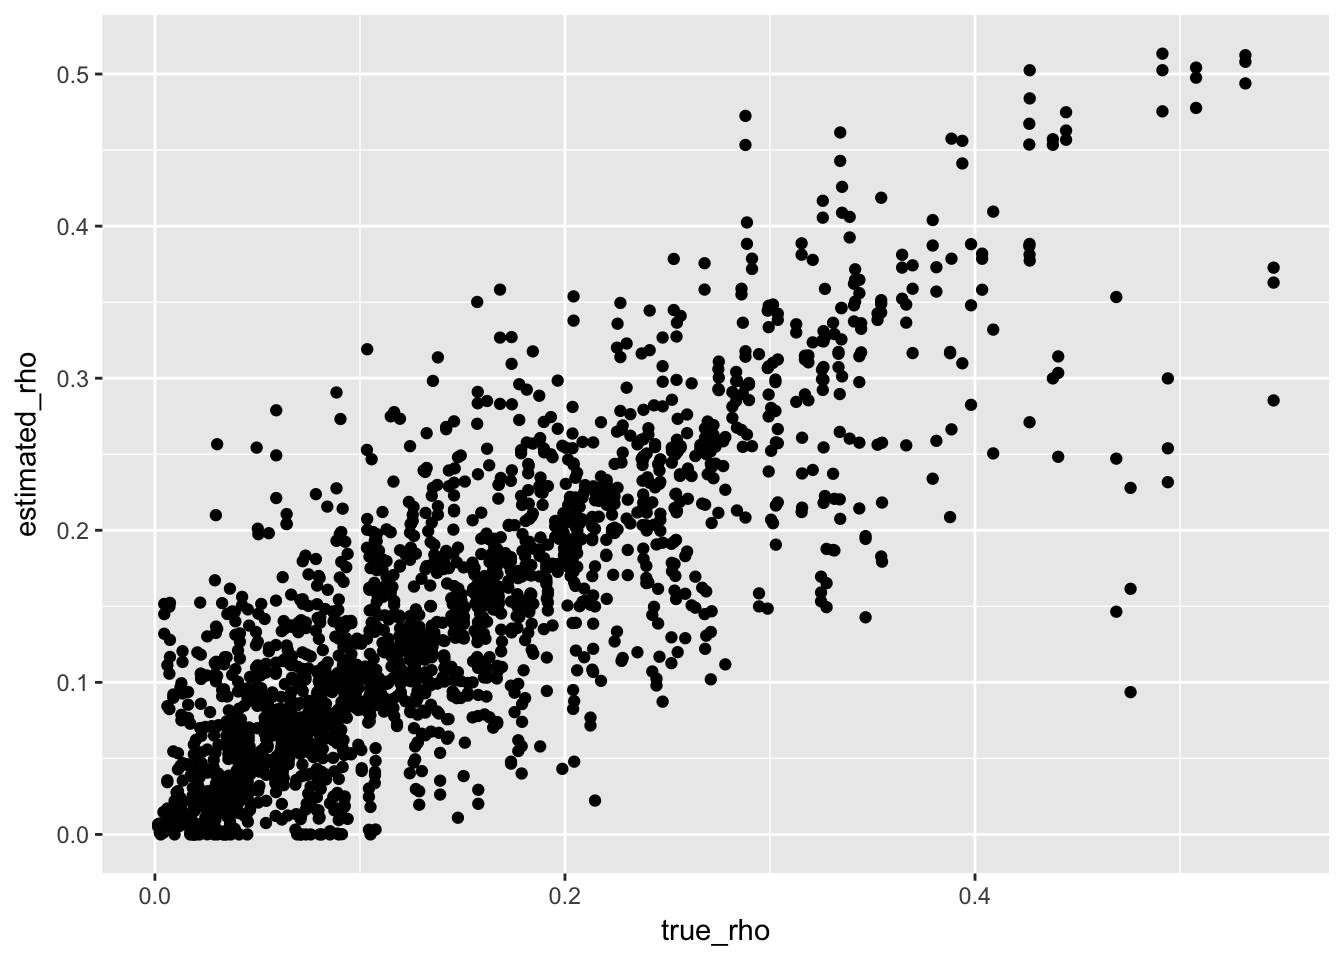
\includegraphics{bookdown-demo_files/figure-latex/unnamed-chunk-34-1.pdf}

OK, that is relatively uninformative. How about we spice it up a bit to
make this:
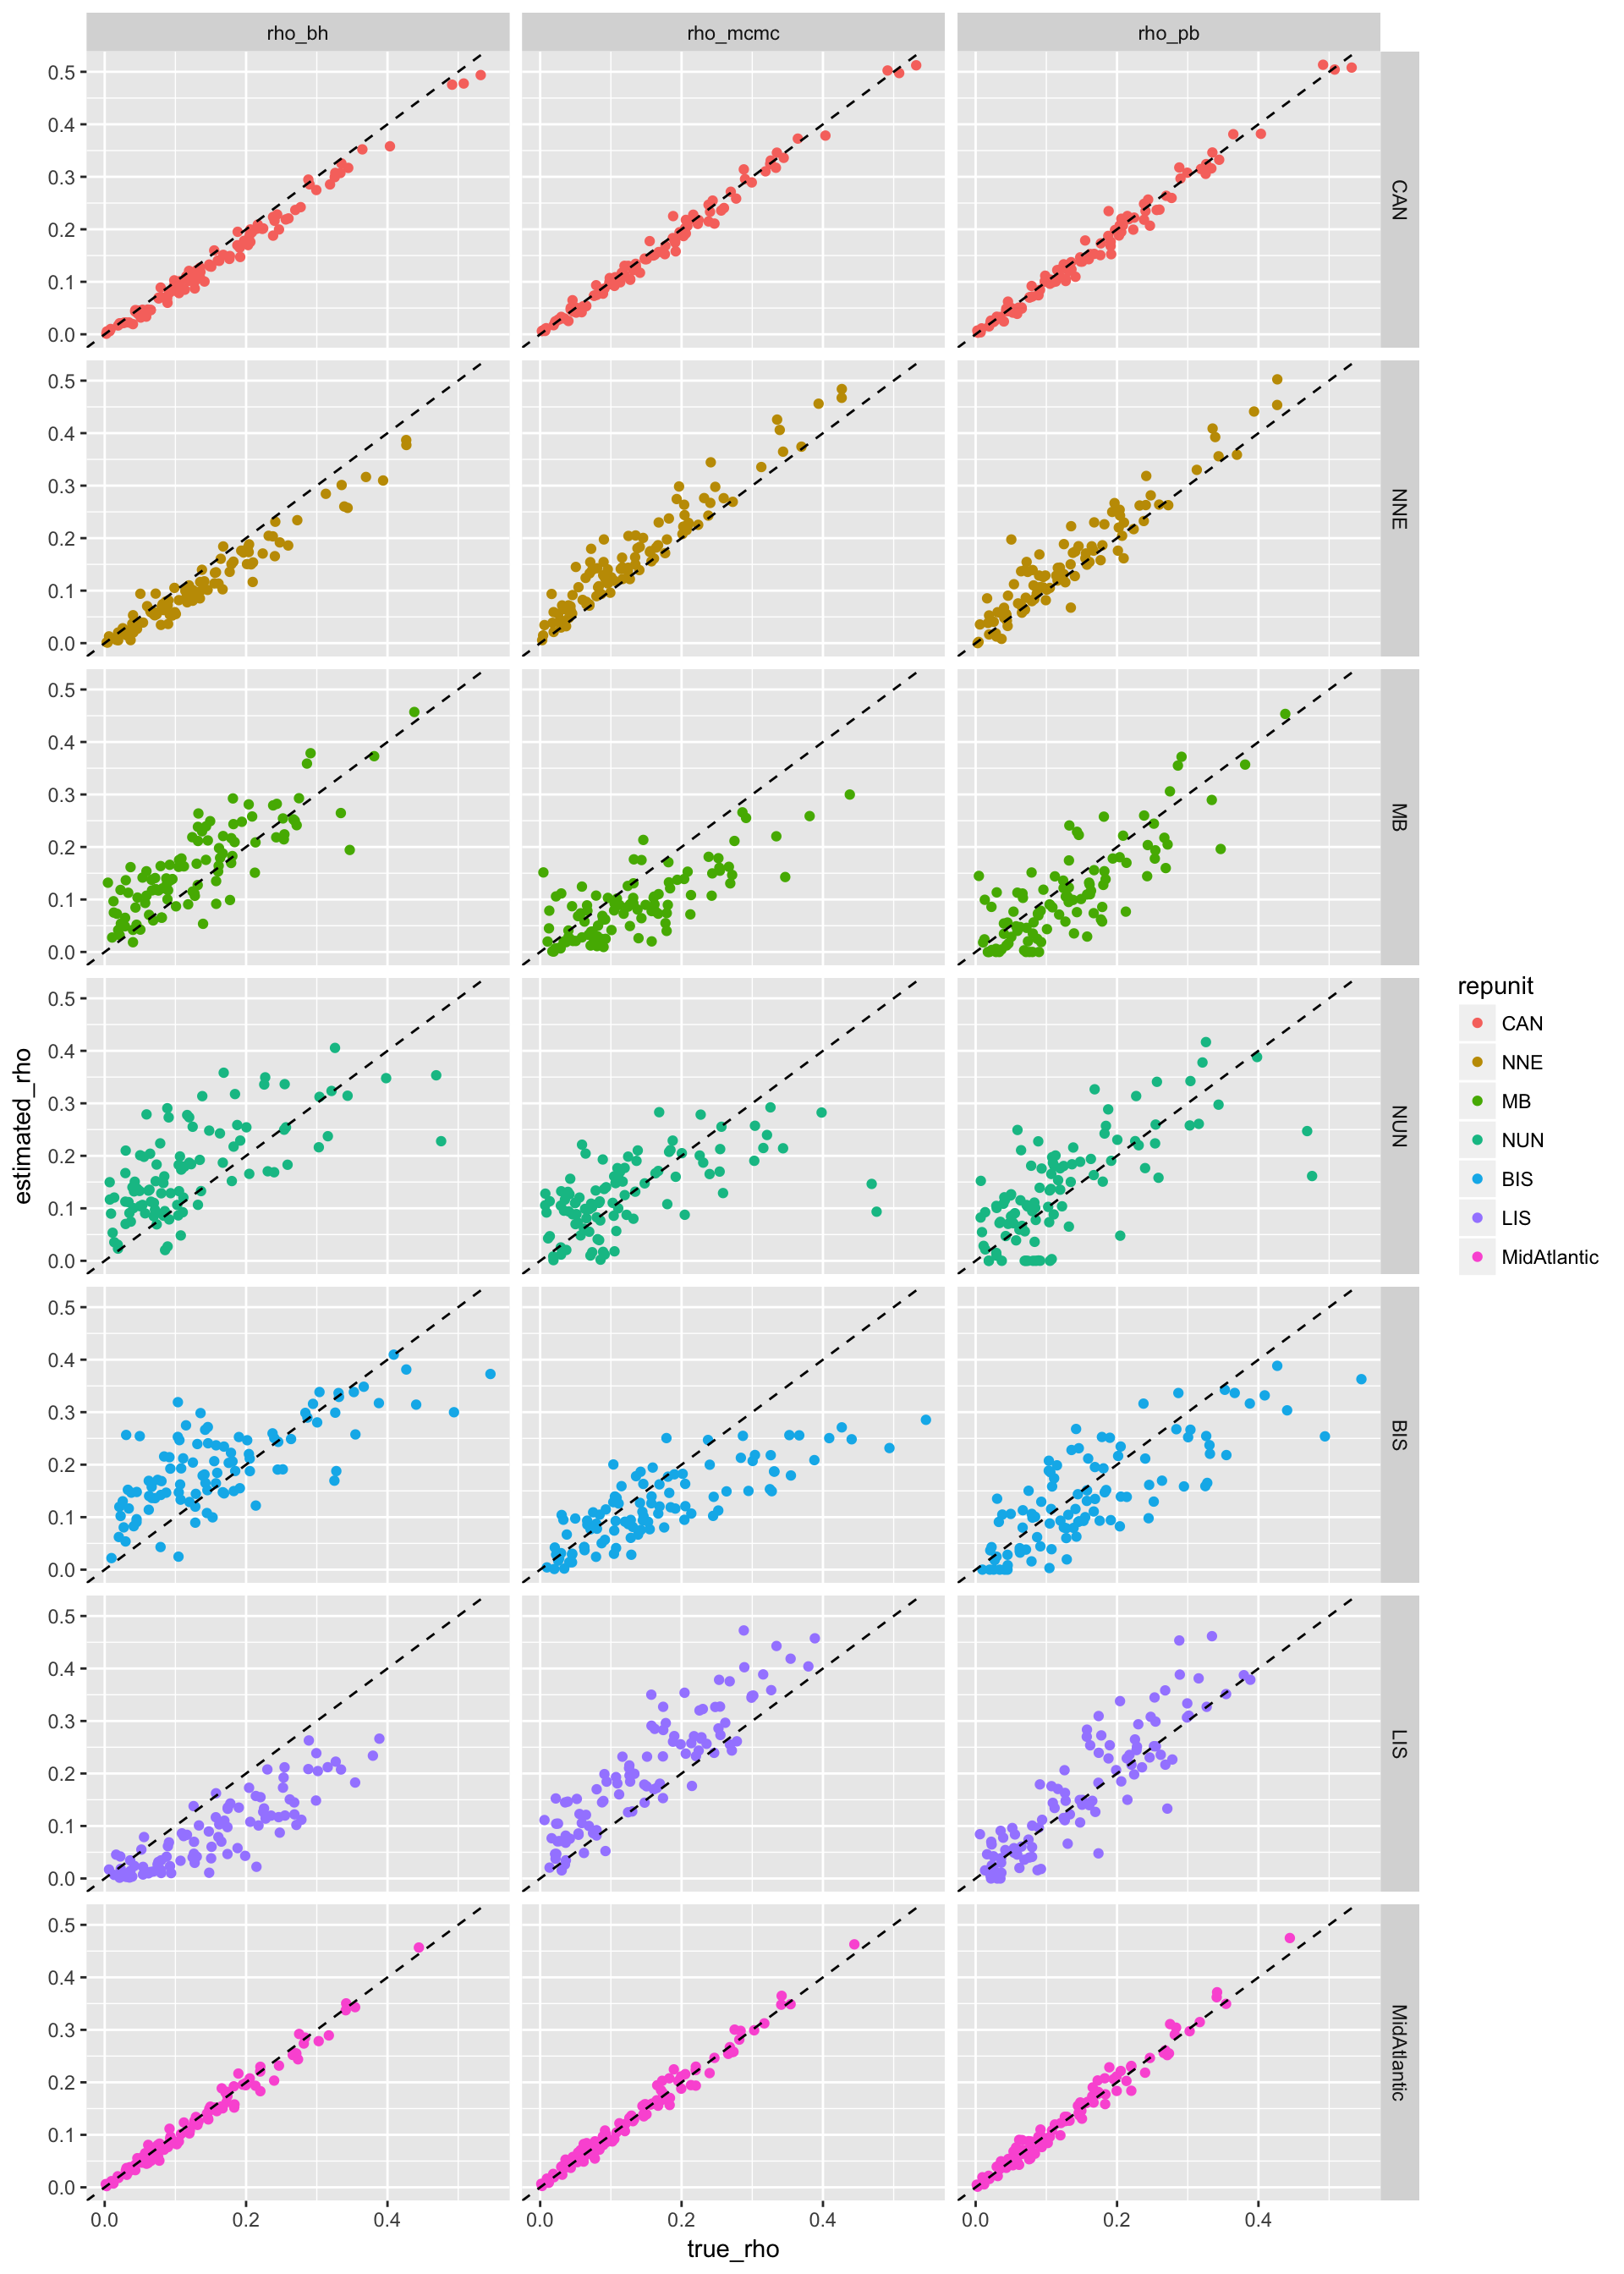
\includegraphics{bookdown-demo_files/figure-latex/unnamed-chunk-35-1.pdf}

\subsection{Your Mission}\label{your-mission}

OK Class! Here is your mission.

\begin{enumerate}
\def\labelenumi{\arabic{enumi}.}
\tightlist
\item
  Download \texttt{tidy\_sims} and figure out during our class time how
  to make the above plot.\\
  Hints: you will be using the \texttt{colour} aesthetic, a
  \texttt{geom\_abline()} geom, and also \texttt{facet\_grid()}
\item
  When you have finished that, use your newly-acquired ggplot skills to
  make an informative plot from your own data set.
\end{enumerate}

I will be here in class to help with this and field any questions.

\section{Some lecture notes from a few years
ago}\label{some-lecture-notes-from-a-few-years-ago}

This is just a rewrite of some playing with ggplot that I did for the
reproducible research course a few years ago, updated to the tidyverse.

It might be worth a reading through to see more examples \#\#\#
Prerequisites \{\#ggplot-prereq\} * To work through the examples you
will need another package that you might not have yet. * Please
download/install these before coming to class: 1. install necessary
packages:

\begin{verbatim}
    ```r
    install.packages("lubridate")
    ```
2. Pull the most recent version of the rep-res-course repo just before coming to class.
\end{verbatim}

\subsection{Goals for this hour:}\label{goals-for-this-hour}

\begin{enumerate}
\def\labelenumi{\arabic{enumi}.}
\tightlist
\item
  Describe (briefly) \texttt{ggplot2}s underlying philosophy and how to
  work with it.
\item
  Quickly overview the \_geom\_s available in \texttt{ggplot2}
\item
  Develop an example plot together
\item
  Turn you all loose with the \texttt{mosaic} package to experiment with
  different plots
\end{enumerate}

\section{About ggplot2}\label{about-ggplot2}

\subsection{Basics}\label{basics}

\begin{itemize}
\tightlist
\item
  A package created by Hadley Wickham in 2005
\item
  Implements Wilkinson's ``grammar of graphics''
\item
  Unified way of thinking about 2-D statistical graphics
\item
  Not entirely easy to learn

  \begin{itemize}
  \tightlist
  \item
    if you already know R's base graphics system, it is painful to
    re-learn a different way of doing things
  \item
    if you don't already know how to do graphics in R, be glad.
  \item
    regardless it is worth learning ggplot
  \item
    I am not even going to teach R's base graphics system
  \end{itemize}
\item
  Amazing for quick data exploration and also produces publication
  quality graphics
\item
  Support for legends etc., considerably better/easier than R base
  graphics
\end{itemize}

\subsection{What is this grammar of
graphics?}\label{what-is-this-grammar-of-graphics}

\begin{itemize}
\tightlist
\item
  Traditionally, people have referred to plots by \emph{name}

  \begin{itemize}
  \tightlist
  \item
    i.e., scatterplot, histogram, bar chart, bubble plot, etc.
  \end{itemize}
\item
  Disadvantages:

  \begin{itemize}
  \tightlist
  \item
    Lots of possible graphics = way too many names
  \item
    Fails to acknowledge the common elements / similarities /
    dissimilarities between different plots
  \end{itemize}
\item
  Wilkinson's \emph{Grammar of Graphics} (a book) describes a few
  building blocks which when assembled together in particular ways can
  generate all these named graphics (and more)

  \begin{itemize}
  \tightlist
  \item
    Provides a nice way of thinking about and describing graphics
  \end{itemize}
\end{itemize}

\subsection{ggplot2}\label{ggplot2}

\begin{itemize}
\tightlist
\item
  Hadley Wickham's R implementation of a modified (\emph{layered})
  grammar of graphics
\item
  \texttt{ggplot} and \texttt{ggplot2} are similar. `\texttt{ggplot2} is
  just more recent (and recommended)
\item
  \texttt{ggplot} operates on \emph{data frames}

  \begin{itemize}
  \tightlist
  \item
    in R base graphics typically you pass in vectors
  \item
    in \texttt{ggplot} everything you want to use in a graphic must be
    contained within a data frame
  \item
    Takes getting used to, but ultimately is a good way of thinking
    about it.
  \end{itemize}
\end{itemize}

\subsection{Components of the grammar of
graphics}\label{components-of-the-grammar-of-graphics}

\begin{enumerate}
\def\labelenumi{\arabic{enumi}.}
\tightlist
\item
  \emph{data} and \emph{aesthetic mappings}
\item
  \emph{geoms} (geometric objects)
\item
  \emph{stats} (statistical transformations)
\item
  \emph{scales}
\item
  \emph{coords} (coordinate systems)
\item
  \emph{facets} (a specification of how to break things into smaller
  subplots)
\end{enumerate}

We will focus on 1, 2 for most of today.

\subsection{In a nutshell}\label{in-a-nutshell}

Without getting into the complications of scales and coordinate systems
here, in a nutshell, is what ggplot does:

\begin{itemize}
\tightlist
\item
  Layers in plots are made by:

  \begin{enumerate}
  \def\labelenumi{\arabic{enumi}.}
  \tightlist
  \item
    mapping \emph{values} in the columns of a data frame to
    \emph{aesthetics}, which are properties that can visually express
    differences, for example:

    \begin{enumerate}
    \def\labelenumii{\alph{enumii}.}
    \tightlist
    \item
      \(x\)-position
    \item
      \(y\)-position
    \item
      shape (of a plot character, for example)
    \item
      color
    \item
      size (of a point, for example)
    \end{enumerate}
  \item
    Portraying those values by drawing a \emph{geometric object} whose
    appearance and placement in space is dictated by the mapping of
    values to aesthetics.
  \end{enumerate}
\end{itemize}

\section{An example, please}\label{pv-example}

Phew! That is a crazy mouthful. Is this really going to help us make
pretty plots?

All I can say is you owe it to yourself to persevere ---
\texttt{ggplot2} is really worth the effort!

\subsection{A pole vaulting example}\label{a-pole-vaulting-example}

\begin{itemize}
\tightlist
\item
  Here is a concrete example: we will investigate the history of
  pole-vaulting world records
\item
  I grabbed the data by copying them from
  \url{http://en.wikipedia.org/wiki/Men's_pole_vault_world_record_progression}
  and pasting them into a text file
\item
  Here we make a data frame out of them:
\end{itemize}

\begin{Shaded}
\begin{Highlighting}[]
\KeywordTok{library}\NormalTok{(tidyverse)  }\CommentTok{# for dealing with dates}
\KeywordTok{library}\NormalTok{(stringr)}
\KeywordTok{library}\NormalTok{(lubridate)  }\CommentTok{# functions mdy, ymd, today(), etc.}
    


\CommentTok{# first off read the data into a data frame}
\NormalTok{pv <-}\StringTok{ }\KeywordTok{read_tsv}\NormalTok{(}\StringTok{"inputs/mens_pole_vault_raw.txt"}\NormalTok{, }\DataTypeTok{comment =} \StringTok{"%"}\NormalTok{) %>%}
\StringTok{  }\KeywordTok{mutate}\NormalTok{(}\DataTypeTok{Date =} \NormalTok{lubridate::}\KeywordTok{mdy}\NormalTok{(}\KeywordTok{str_replace}\NormalTok{(Date, }\StringTok{"}\CharTok{\textbackslash{}\textbackslash{}}\StringTok{[[0-9]}\CharTok{\textbackslash{}\textbackslash{}}\StringTok{]"}\NormalTok{, }\StringTok{""}\NormalTok{))) %>%}\StringTok{ }\CommentTok{# clean up dates}
\StringTok{  }\KeywordTok{mutate}\NormalTok{(}\DataTypeTok{Meters =} \KeywordTok{parse_number}\NormalTok{(Record))  }\CommentTok{# get the record in a numeric number of meters}
\end{Highlighting}
\end{Shaded}

\begin{verbatim}
## Parsed with column specification:
## cols(
##   Record = col_character(),
##   Athlete = col_character(),
##   Nation = col_character(),
##   Venue = col_character(),
##   Date = col_character(),
##   `#[2]` = col_integer()
## )
\end{verbatim}

\begin{itemize}
\tightlist
\item
  Great, what do these look like? Try \texttt{View(pv)} if you are
  following along. Here are the first few rows too:
\end{itemize}

\begin{Shaded}
\begin{Highlighting}[]
\NormalTok{pv}
\end{Highlighting}
\end{Shaded}

\begin{verbatim}
## # A tibble: 72 × 7
##    Record        Athlete        Nation               Venue       Date
##     <chr>          <chr>         <chr>               <chr>     <date>
## 1  4.02 m    Marc Wright United States     Cambridge, U.S. 1912-06-08
## 2  4.09 m     Frank Foss United States    Antwerp, Belgium 1920-08-20
## 3  4.12 m   Charles Hoff        Norway Copenhagen, Denmark 1922-09-22
## 4  4.21 m   Charles Hoff        Norway Copenhagen, Denmark 1923-07-22
## 5  4.23 m   Charles Hoff        Norway        Oslo, Norway 1925-08-13
## 6  4.25 m   Charles Hoff        Norway      Turku, Finland 1925-09-27
## 7  4.27 m     Sabin Carr United States  Philadelphia, U.S. 1927-05-27
## 8  4.30 m     Lee Barnes United States        Fresno, U.S. 1928-04-28
## 9  4.37 m William Graber United States     Palo Alto, U.S. 1932-07-16
## 10 4.39 m    Keith Brown United States        Boston, U.S. 1935-06-01
## # ... with 62 more rows, and 2 more variables: `#[2]` <int>, Meters <dbl>
\end{verbatim}

\subsection{A first ggplot}\label{a-first-ggplot}

\begin{itemize}
\tightlist
\item
  There is a simplified ggplot function called \texttt{qplot} that
  behaves more like R's base graphics function \texttt{plot()}.

  \begin{itemize}
  \tightlist
  \item
    I don't recommend \texttt{qplot}. It will just lengthen the time it
    takes to understand the grammar of graphics.
  \item
    Instead, we will use the full \texttt{ggplot()} standard syntax.
  \end{itemize}
\end{itemize}

\begin{enumerate}
\def\labelenumi{\arabic{enumi}.}
\item
  First we have to essentially establish a plotting area upon which to
  add layers. We will do this like so:

\begin{Shaded}
\begin{Highlighting}[]
\NormalTok{g <-}\StringTok{ }\KeywordTok{ggplot}\NormalTok{()}
\end{Highlighting}
\end{Shaded}

  At this point, \texttt{g} is a ggplot plot object. We can try printing
  it:

\begin{Shaded}
\begin{Highlighting}[]
\NormalTok{g}
\end{Highlighting}
\end{Shaded}

  
\includegraphics{bookdown-demo_files/figure-latex/unnamed-chunk-40-1.pdf}
  That doesn't work, because there is nothing to plot. We have to add a
  layer to it.
\item
  Adding a layer is done by adding a collection of geometric objects to
  it using one of the \texttt{geom\_xxxx} functions. Each such function
  requires a \emph{data set} and a \emph{mapping} of columns in the data
  set to \emph{aesthetics}. Let's make some scatter-points: Meters as a
  function of Date:

\begin{Shaded}
\begin{Highlighting}[]
\NormalTok{g2 <-}\StringTok{ }\NormalTok{g +}\StringTok{ }\KeywordTok{geom_point}\NormalTok{(}\DataTypeTok{data =} \NormalTok{pv, }\DataTypeTok{mapping =} \KeywordTok{aes}\NormalTok{(}\DataTypeTok{x =} \NormalTok{Date, }\DataTypeTok{y =} \NormalTok{Meters))}
\NormalTok{g2}
\end{Highlighting}
\end{Shaded}

  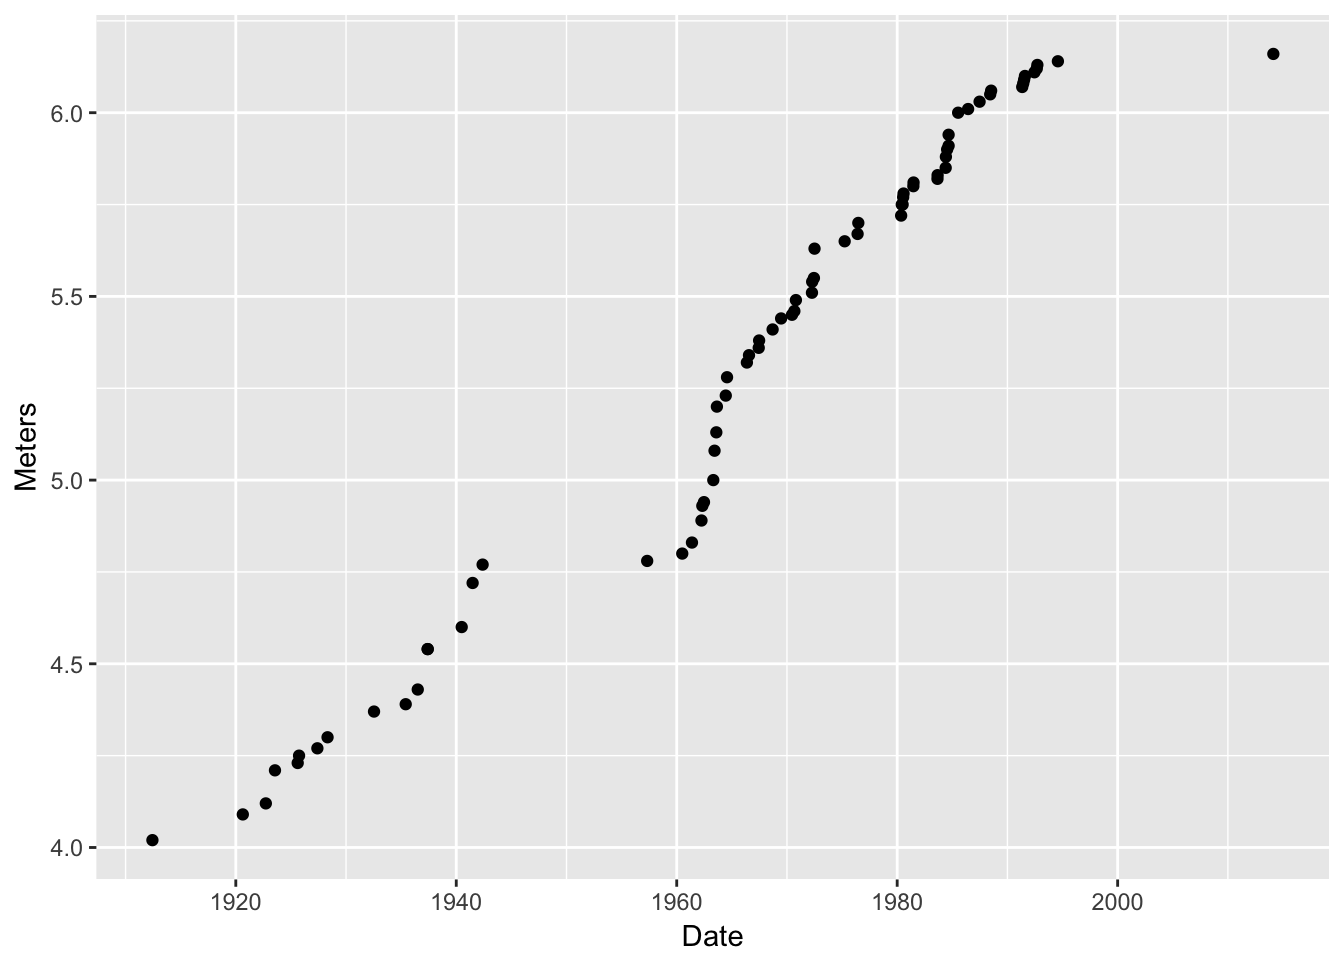
\includegraphics{bookdown-demo_files/figure-latex/unnamed-chunk-41-1.pdf}

  Wow! That totally worked. Here are some interesting points about:

\begin{Shaded}
\begin{Highlighting}[]
\NormalTok{g2 <-}\StringTok{ }\NormalTok{g +}\StringTok{ }\KeywordTok{geom_point}\NormalTok{(}\DataTypeTok{data =} \NormalTok{pv, }\DataTypeTok{mapping =} \KeywordTok{aes}\NormalTok{(}\DataTypeTok{x =} \NormalTok{Date, }\DataTypeTok{y =} \NormalTok{Meters))}
\NormalTok{g2}
\end{Highlighting}
\end{Shaded}

  \begin{enumerate}
  \def\labelenumii{\alph{enumii}.}
  \tightlist
  \item
    You add layers by catenating them with \texttt{+}.
  \item
    the names of the columns don't need to be quoted.
  \item
    when you map aesthestics you wrap them inside the \texttt{aes()}
    function
  \item
    the full object with all the layers is returned into \texttt{g2} and
    then we printed it (by typing \texttt{g2}). (we could have also just
    said
    \texttt{g\ +\ geom\_point(data\ =\ pv,\ mapping\ =\ aes(x\ =\ Date,\ y\ =\ Meters))})
  \item
    we didn't have to do anything fancy to the dates\ldots{}ggplot knew
    how to plot them. This is thanks to turning the dates into
    \texttt{lubridate} objects. (If you work with dates, get to know the
    lubridate package!)
  \end{enumerate}
\item
  I want to overlay a line on that\ldots{}No problem! Add another layer:

\begin{Shaded}
\begin{Highlighting}[]
\NormalTok{g3 <-}\StringTok{ }\NormalTok{g2 +}\StringTok{ }\KeywordTok{geom_line}\NormalTok{(}\DataTypeTok{data =} \NormalTok{pv, }\DataTypeTok{mapping =} \KeywordTok{aes}\NormalTok{(}\DataTypeTok{x =} \NormalTok{Date, }\DataTypeTok{y =} \NormalTok{Meters))}
\NormalTok{g3}
\end{Highlighting}
\end{Shaded}

  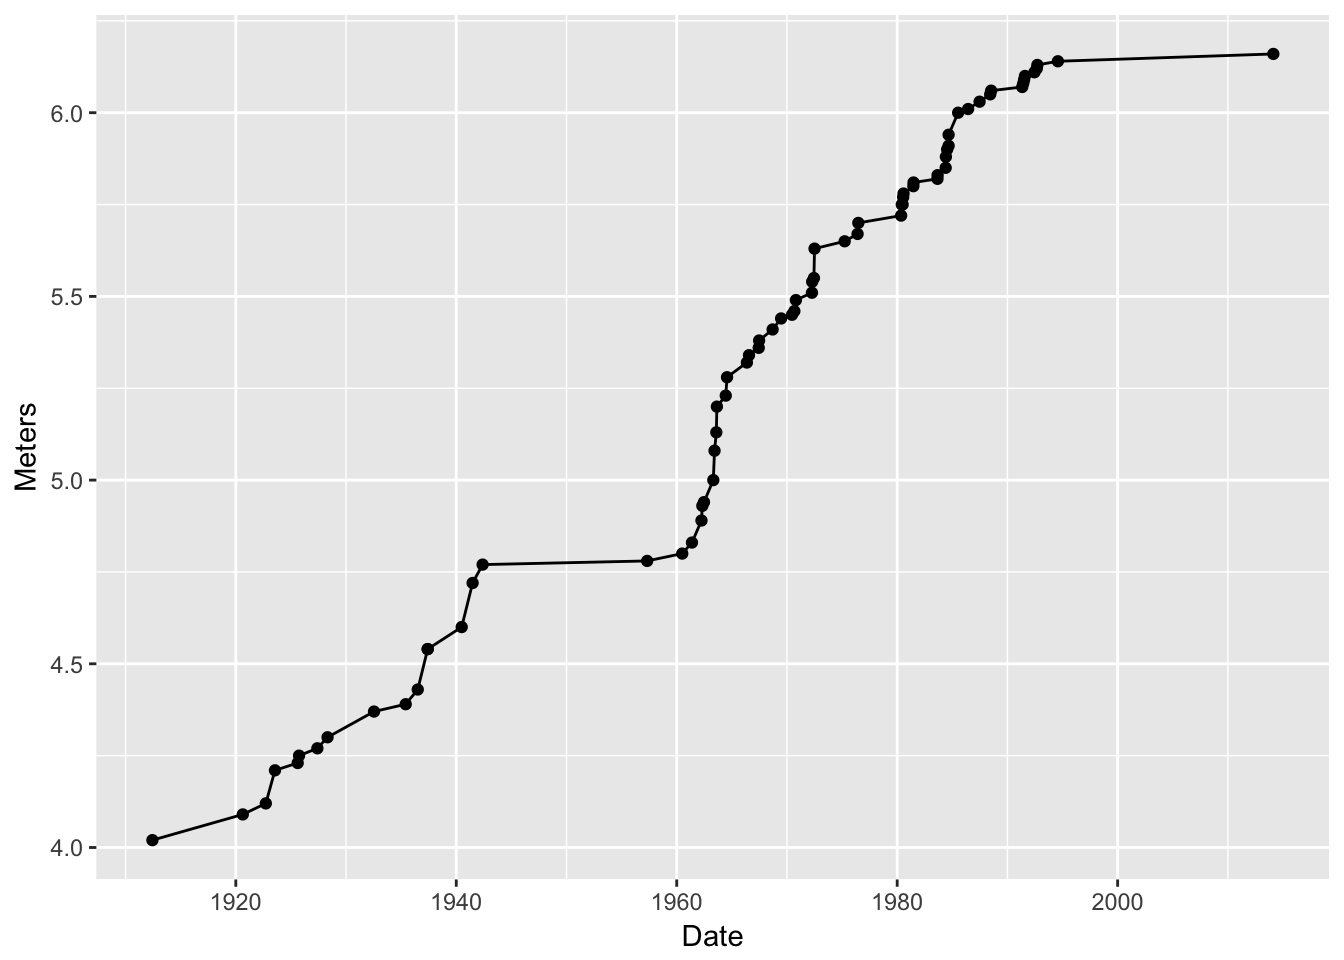
\includegraphics{bookdown-demo_files/figure-latex/unnamed-chunk-43-1.pdf}

  That worked! We just added (literally, using a \texttt{+} sign!)
  another layer---one that had a line on it. BUT! what if I want to make
  that line blue?
\item
  Make the line blue. Note that you are giving the line an aesthetic
  property (the color blue), but you are not mapping that to any values
  in the data frame, \textbf{so} you don't put that within the
  \texttt{aes()} function:

\begin{Shaded}
\begin{Highlighting}[]
\NormalTok{g4 <-}\StringTok{ }\NormalTok{g2 +}\StringTok{ }\KeywordTok{geom_line}\NormalTok{(}\DataTypeTok{data =} \NormalTok{pv, }\DataTypeTok{mapping =} \KeywordTok{aes}\NormalTok{(}\DataTypeTok{x =} \NormalTok{Date, }\DataTypeTok{y =} \NormalTok{Meters), }\DataTypeTok{color =} \StringTok{"blue"}\NormalTok{)}
\NormalTok{g4}
\end{Highlighting}
\end{Shaded}

  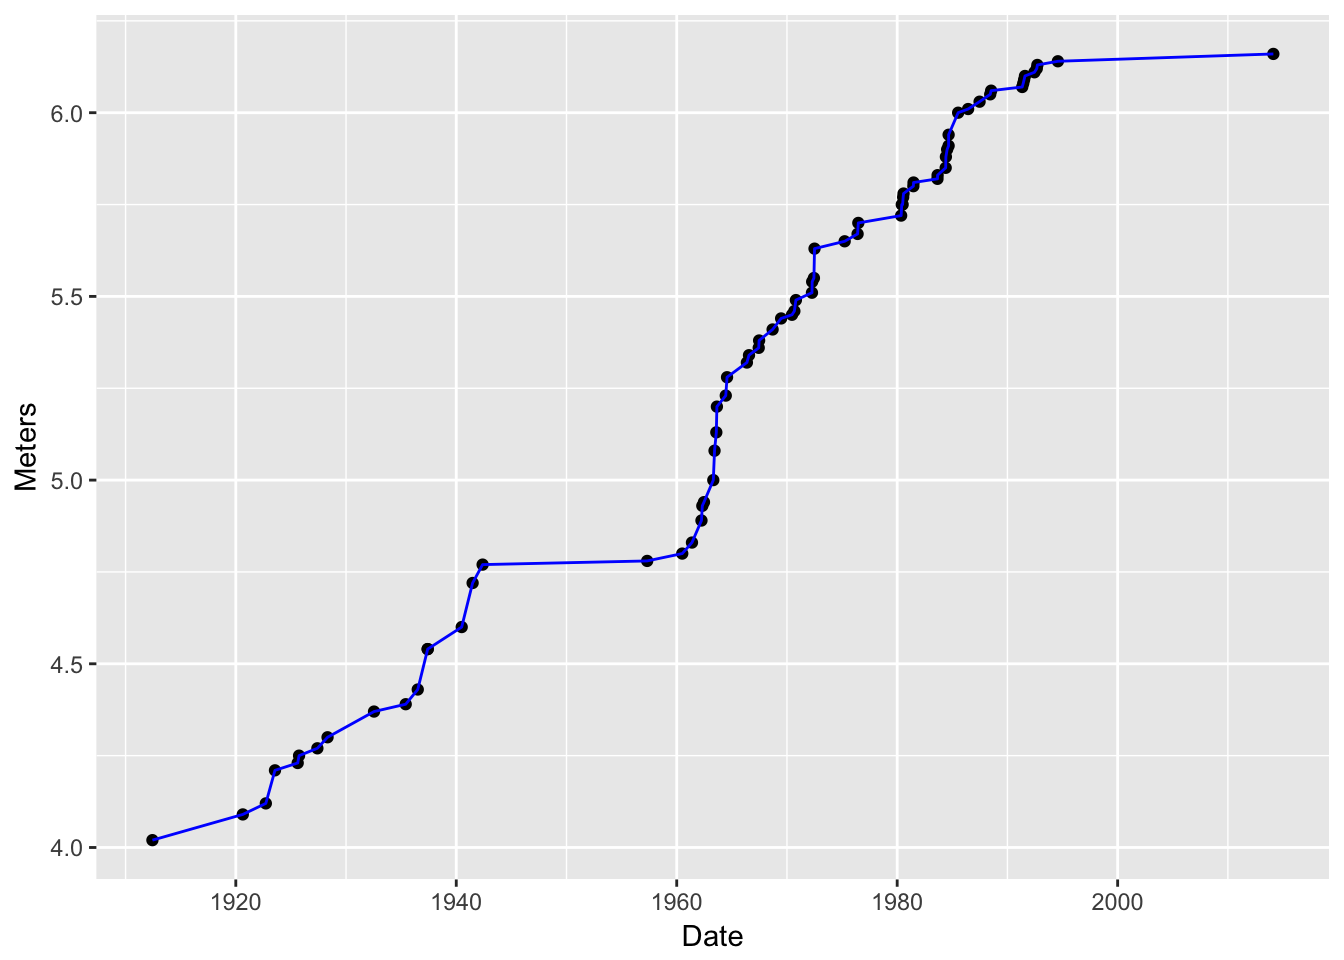
\includegraphics{bookdown-demo_files/figure-latex/unnamed-chunk-44-1.pdf}

  That worked! Notice that we were able to put that new layer atop
  \texttt{g2} which we had stored previously.
\end{enumerate}

\subsection{ggplot's system of
defaults}\label{ggplots-system-of-defaults}

\begin{itemize}
\item
  Hey! I am really tired of typing
  \texttt{data\ =\ pv,\ mapping\ =\ aes(x\ =\ Date,\ y\ =\ Meters)}
  isn't there some way around that?
\item
  Yes! You can pass a default data frame and/or default mappings to the
  original \texttt{ggplot()} function. Then, if data and mappings are
  not specified in later layers, the defaults are used.
\item
  Witness!

\begin{Shaded}
\begin{Highlighting}[]
\NormalTok{d <-}\StringTok{ }\KeywordTok{ggplot}\NormalTok{(}\DataTypeTok{data =} \NormalTok{pv, }\KeywordTok{aes}\NormalTok{(}\DataTypeTok{x =} \NormalTok{Date, }\DataTypeTok{y =} \NormalTok{Meters))  }\CommentTok{# this defines defaults}
\NormalTok{d2 <-}\StringTok{ }\NormalTok{d +}\StringTok{ }\KeywordTok{geom_point}\NormalTok{()  }\CommentTok{# add a layer with points}
\NormalTok{d2  }\CommentTok{# print it}
\end{Highlighting}
\end{Shaded}

  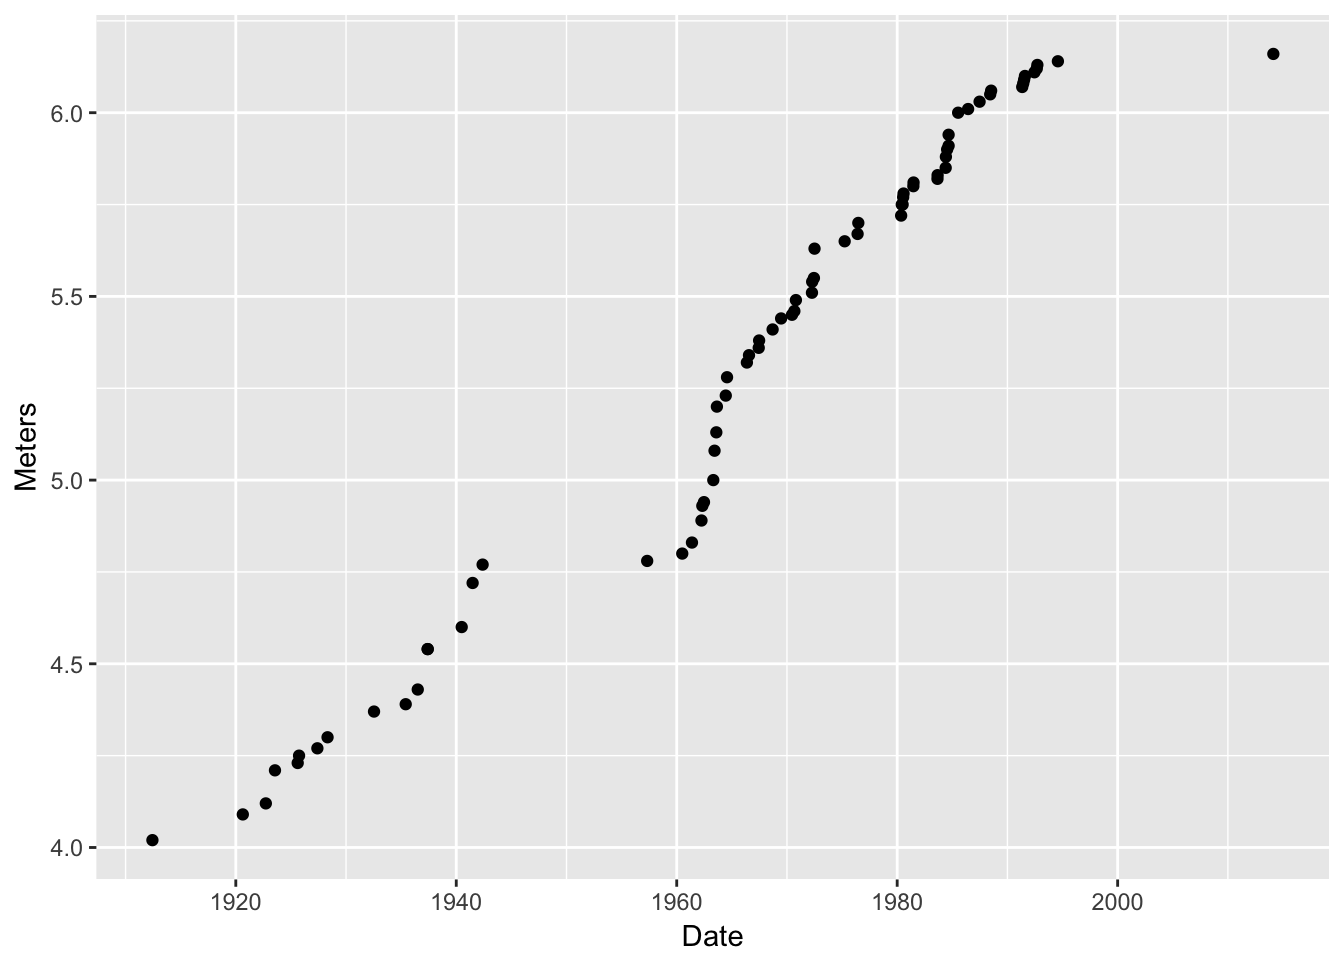
\includegraphics{bookdown-demo_files/figure-latex/unnamed-chunk-45-1.pdf}
\item
  Sick! Now we can add all sorts of fun layers as we see fit, each time,
  by invoking a \texttt{geom\_xxx()} function.
\item
  Let's go totally crazy!
\end{itemize}

\begin{enumerate}
\def\labelenumi{\arabic{enumi}.}
\item
  Establish plot base with defaults:

\begin{Shaded}
\begin{Highlighting}[]
\NormalTok{d <-}\StringTok{ }\KeywordTok{ggplot}\NormalTok{(}\DataTypeTok{data =} \NormalTok{pv, }\KeywordTok{aes}\NormalTok{(}\DataTypeTok{x =} \NormalTok{Date, }\DataTypeTok{y =} \NormalTok{Meters))}
\end{Highlighting}
\end{Shaded}
\item
  Add a transparent turquoise area along the back:

\begin{Shaded}
\begin{Highlighting}[]
\NormalTok{d2 <-}\StringTok{ }\NormalTok{d +}\StringTok{ }\KeywordTok{geom_ribbon}\NormalTok{(}\KeywordTok{aes}\NormalTok{(}\DataTypeTok{ymax =} \NormalTok{Meters), }\DataTypeTok{ymin =} \KeywordTok{min}\NormalTok{(pv$Meters), }\DataTypeTok{alpha =} \FloatTok{0.4}\NormalTok{, }\DataTypeTok{fill =} \StringTok{"turquoise"}\NormalTok{)}
\NormalTok{d2}
\end{Highlighting}
\end{Shaded}

  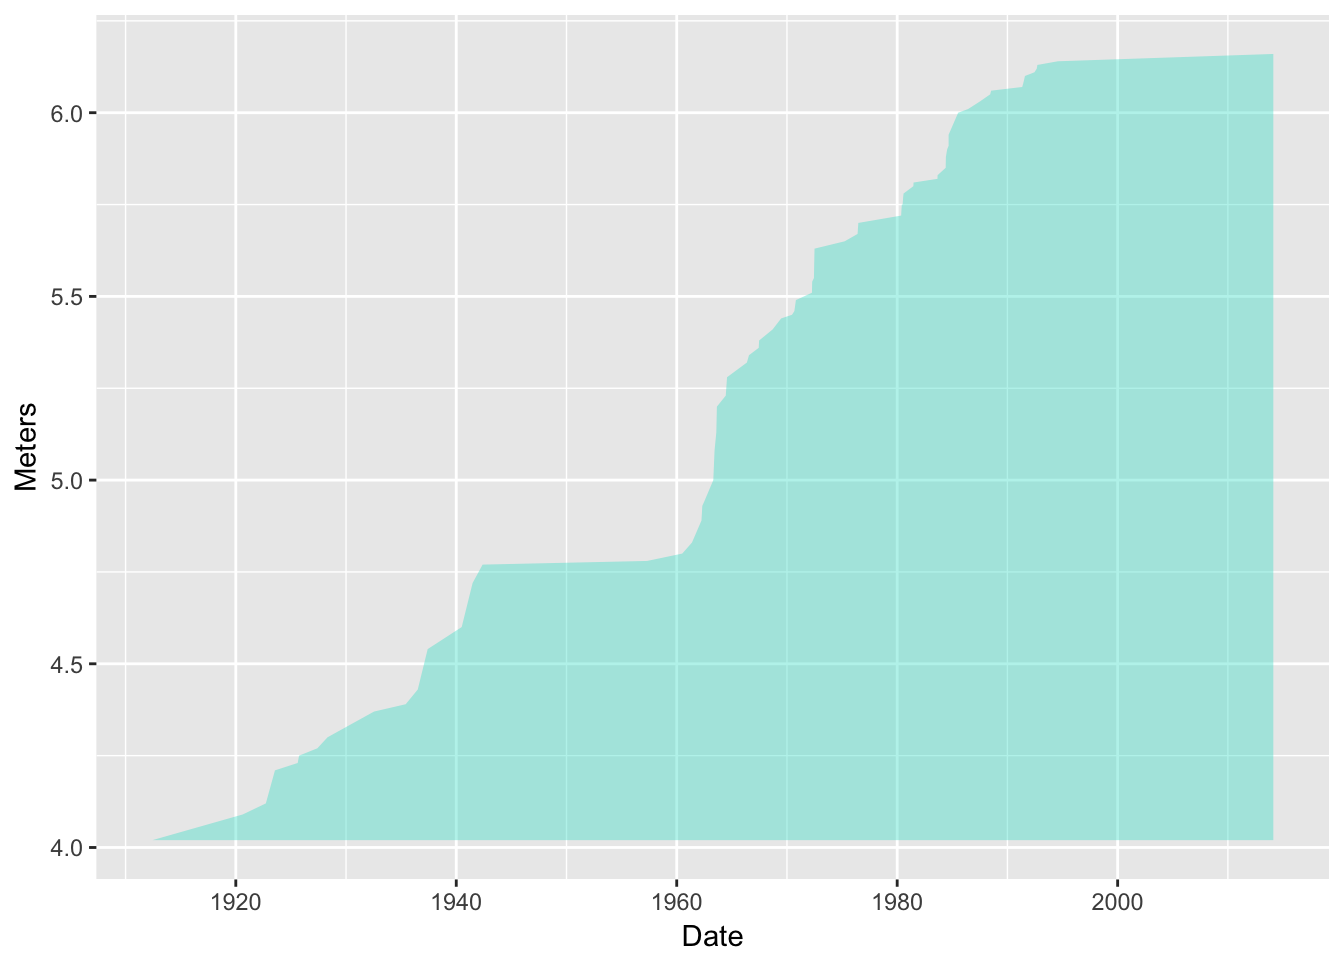
\includegraphics{bookdown-demo_files/figure-latex/unnamed-chunk-47-1.pdf}

  Wow! I feel like transparency was never so easy in R base graphics!
\item
  Put a line along there too:

\begin{Shaded}
\begin{Highlighting}[]
\NormalTok{d3 <-}\StringTok{ }\NormalTok{d2 +}\StringTok{ }\KeywordTok{geom_line}\NormalTok{(}\DataTypeTok{color =} \StringTok{"blue"}\NormalTok{)}
\NormalTok{d3}
\end{Highlighting}
\end{Shaded}

  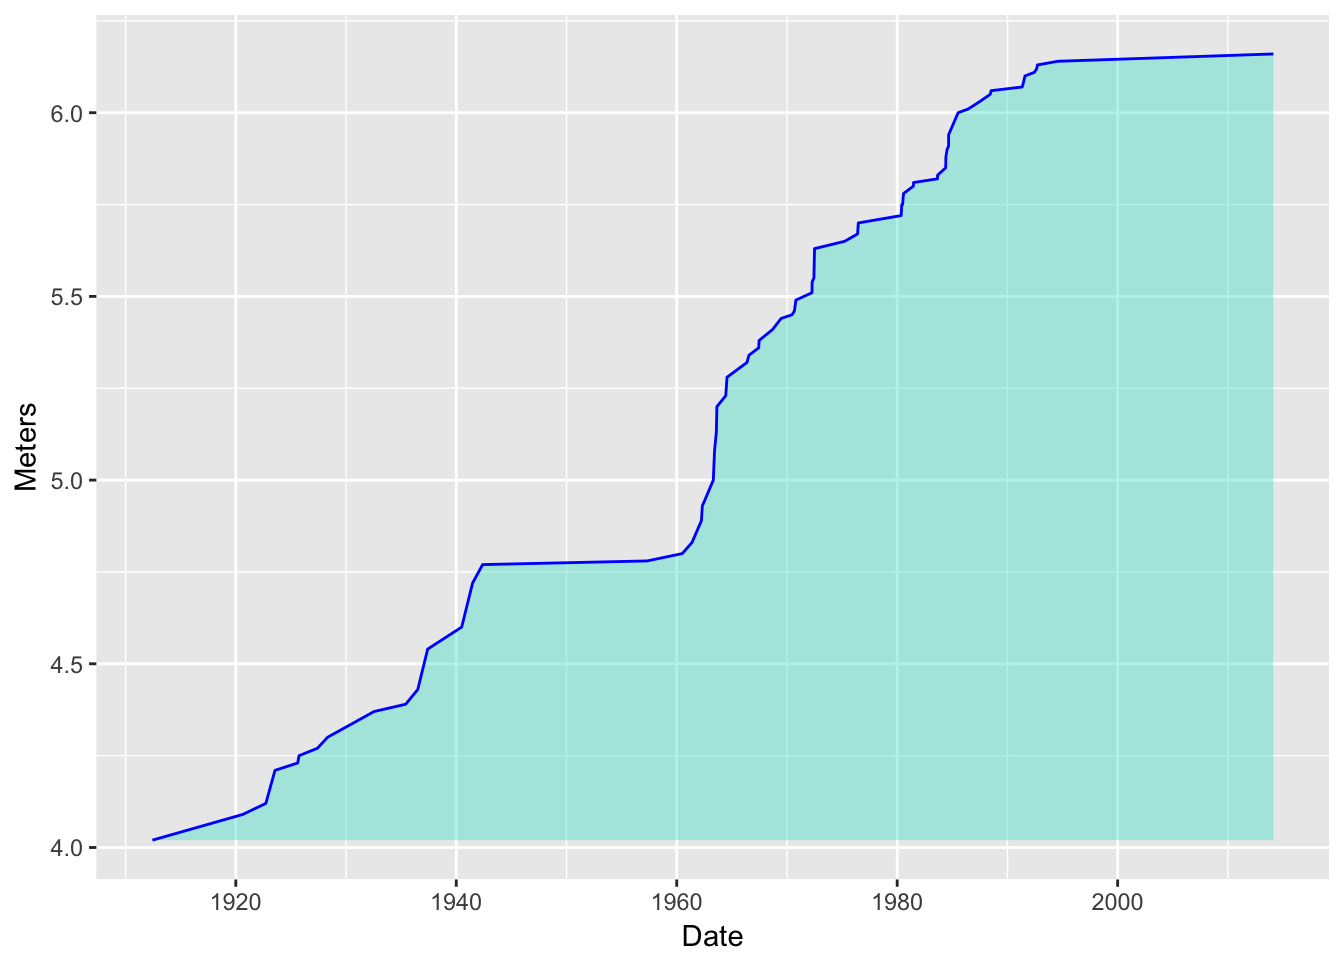
\includegraphics{bookdown-demo_files/figure-latex/unnamed-chunk-48-1.pdf}
\item
  Now add some small orange points:

\begin{Shaded}
\begin{Highlighting}[]
\NormalTok{d4 <-}\StringTok{ }\NormalTok{d3 +}\StringTok{ }\KeywordTok{geom_point}\NormalTok{(}\DataTypeTok{color =} \StringTok{"orange"}\NormalTok{)}
\NormalTok{d4}
\end{Highlighting}
\end{Shaded}

  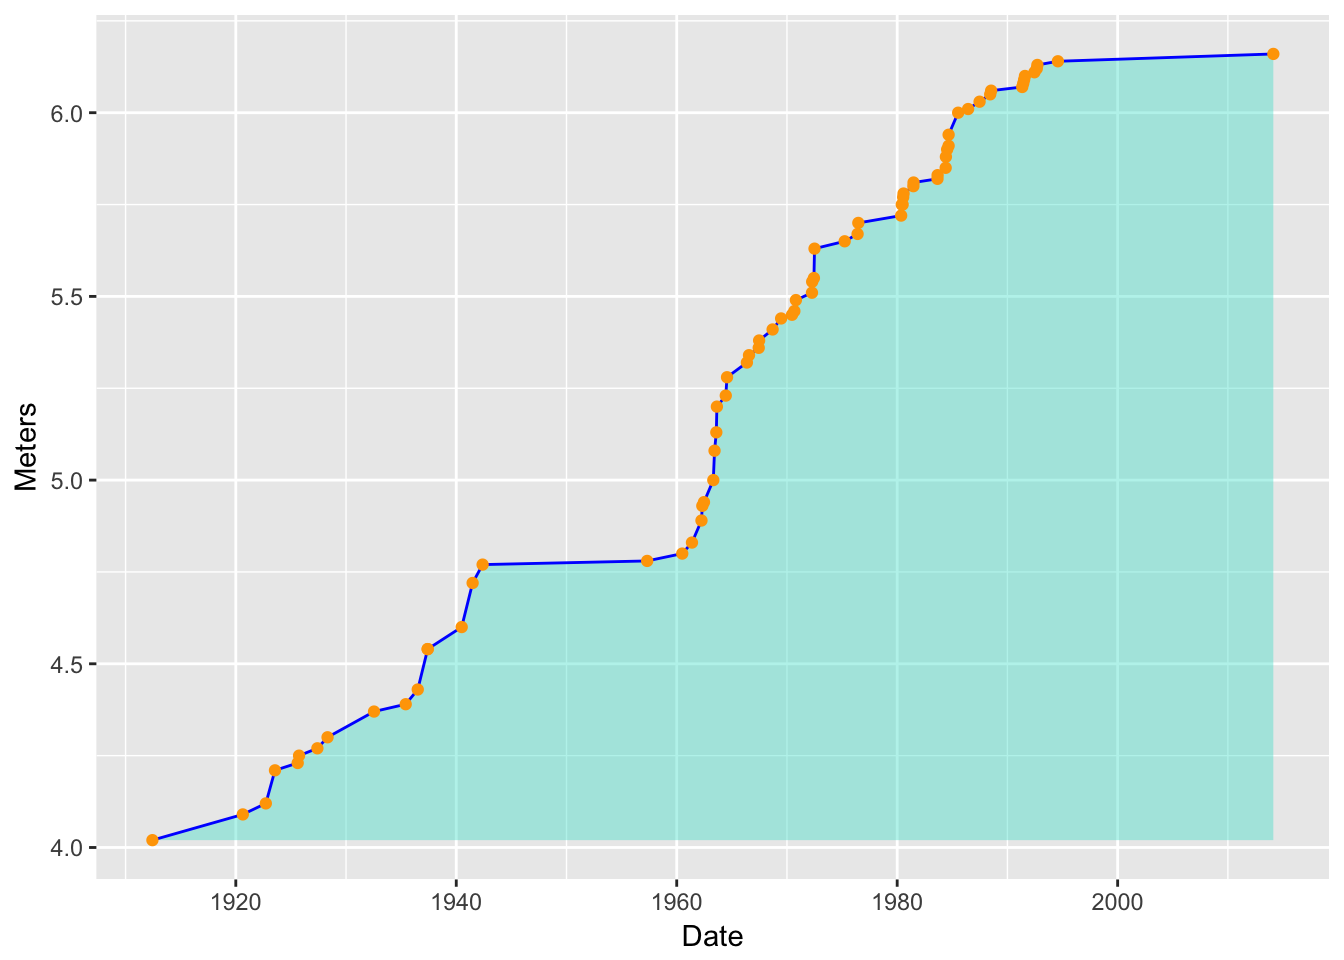
\includegraphics{bookdown-demo_files/figure-latex/unnamed-chunk-49-1.pdf}
\item
  Now, add ``rugs'' along the \(x\) and \(y\) axes that show the
  position of points, and in them, map \emph{color} to \emph{Nation}:

\begin{Shaded}
\begin{Highlighting}[]
\NormalTok{d5 <-}\StringTok{ }\NormalTok{d4 +}\StringTok{ }\KeywordTok{geom_rug}\NormalTok{(}\DataTypeTok{sides =} \StringTok{"bl"}\NormalTok{, }\DataTypeTok{mapping =} \KeywordTok{aes}\NormalTok{(}\DataTypeTok{color =} \NormalTok{Nation))}
\NormalTok{d5}
\end{Highlighting}
\end{Shaded}

  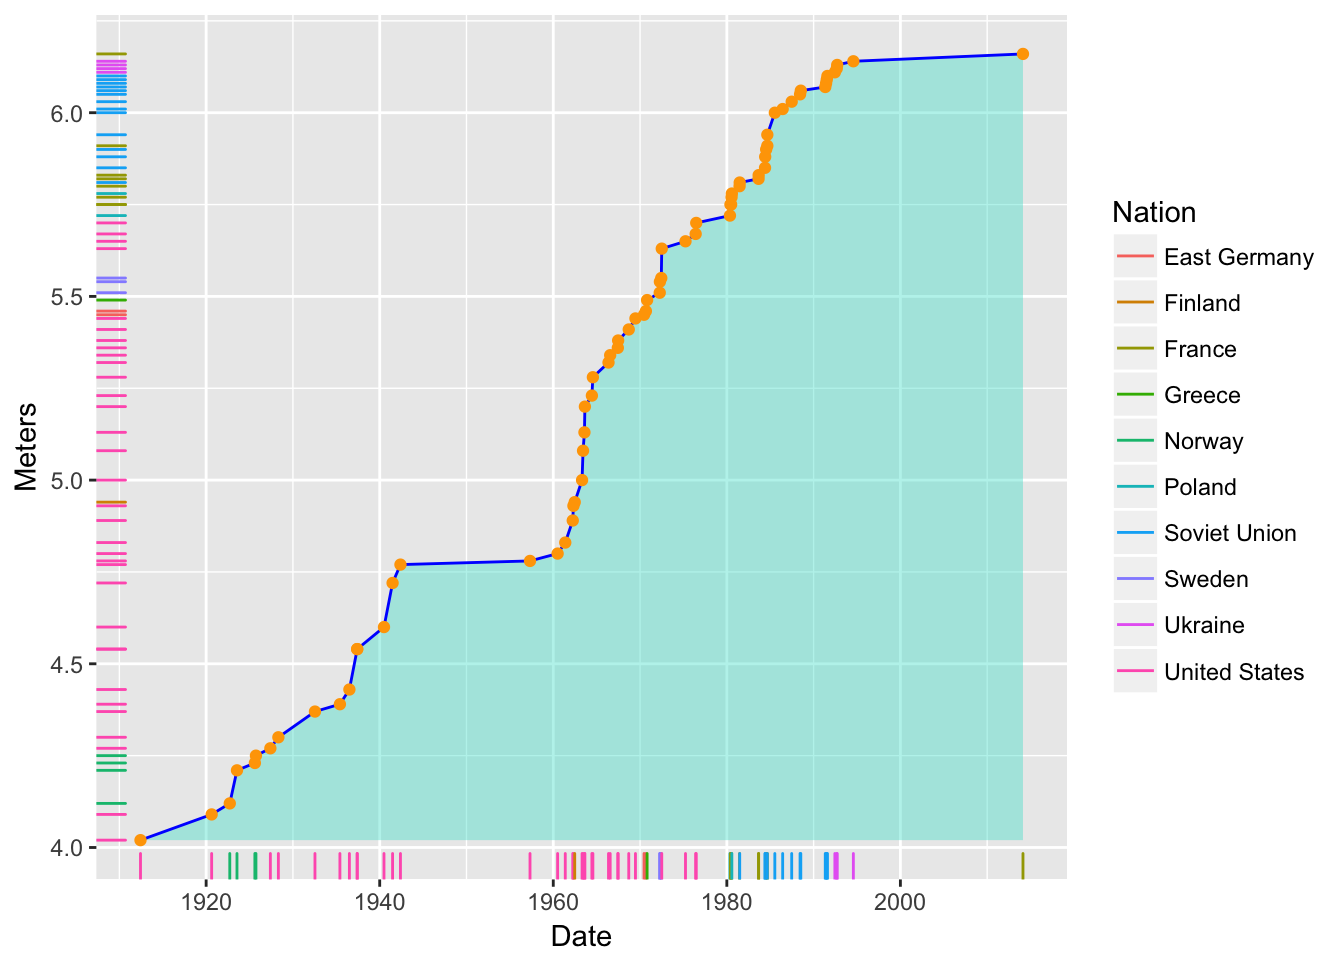
\includegraphics{bookdown-demo_files/figure-latex/unnamed-chunk-50-1.pdf}

  \begin{itemize}
  \tightlist
  \item
    Note that we are using the \texttt{aes()} function to add the
    mapping of \emph{color} to \emph{Nation} within the
    \texttt{geom\_rug()} function.

    \begin{itemize}
    \tightlist
    \item
      Note also that the legend was created automatically.
    \end{itemize}
  \item
    Wow! A legend is produced automatically, by default, and it looks
    pretty good. This doesn't happen without an all-out wrestling match
    in R's base graphics system.
  \end{itemize}
\end{enumerate}

\begin{itemize}
\tightlist
\item
  So, that was some fun playing around with the truly awesome ease with
  which you can build up complex and lovely graphics with ggplot.
\end{itemize}

\subsection{How many geoms are there?}\label{how-many-geoms-are-there}

\begin{itemize}
\tightlist
\item
  Quite a few. There is a good summary with little icons for each
  \href{http://docs.ggplot2.org/current/}{here}
\item
  Note that most geoms respond to the aesthetics of \texttt{x},
  \texttt{y}, and \texttt{color} (or \texttt{fill}). And some have more
  (or other) aesthetics you can map values to.
\end{itemize}

\subsection{Getting even sillier}\label{getting-even-sillier}

\begin{itemize}
\tightlist
\item
  Here is another plot I made while geeking out.
\item
  I wanted to get a sense for how much individual athletes had improved
  since their first world record
\end{itemize}

\begin{Shaded}
\begin{Highlighting}[]
\CommentTok{# add a column for the date of first record for each athlete}
\NormalTok{pv <-}\StringTok{ }\NormalTok{pv %>%}
\StringTok{  }\KeywordTok{group_by}\NormalTok{(Athlete) %>%}
\StringTok{  }\KeywordTok{mutate}\NormalTok{(}\DataTypeTok{FirstRecordMeters =} \KeywordTok{min}\NormalTok{(Meters)) %>%}\StringTok{ }
\StringTok{  }\KeywordTok{ungroup}\NormalTok{() %>%}
\StringTok{  }\KeywordTok{mutate}\NormalTok{(}\DataTypeTok{DateNext =} \KeywordTok{lead}\NormalTok{(Date,  }\DataTypeTok{default =} \NormalTok{lubridate::}\KeywordTok{ymd}\NormalTok{(lubridate::}\KeywordTok{today}\NormalTok{())))}


\NormalTok{bb <-}\StringTok{ }\KeywordTok{ggplot}\NormalTok{(}\DataTypeTok{data =} \NormalTok{pv, }\DataTypeTok{mapping =} \KeywordTok{aes}\NormalTok{(}\DataTypeTok{x =} \NormalTok{Date, }\DataTypeTok{y =} \NormalTok{Meters, }\DataTypeTok{color =} \NormalTok{Nation))  +}\StringTok{ }
\StringTok{  }\KeywordTok{geom_ribbon}\NormalTok{(}\KeywordTok{aes}\NormalTok{(}\DataTypeTok{ymax =} \NormalTok{Meters, }\DataTypeTok{color =} \OtherTok{NULL}\NormalTok{), }\DataTypeTok{ymin =} \KeywordTok{min}\NormalTok{(pv$Meters), }\DataTypeTok{alpha =} \FloatTok{0.2}\NormalTok{, }\DataTypeTok{fill =} \StringTok{"orange"}\NormalTok{) +}
\StringTok{  }\KeywordTok{geom_line}\NormalTok{(}\DataTypeTok{color =} \StringTok{"black"}\NormalTok{, }\DataTypeTok{size =} \NormalTok{.}\DecValTok{1}\NormalTok{) +}
\StringTok{  }\KeywordTok{geom_rect}\NormalTok{(}\KeywordTok{aes}\NormalTok{(}\DataTypeTok{xmin =} \NormalTok{Date, }
                \DataTypeTok{xmax =} \NormalTok{DateNext, }
                \DataTypeTok{ymin =} \NormalTok{FirstRecordMeters, }
                \DataTypeTok{ymax =} \NormalTok{Meters,}
                \DataTypeTok{fill =} \NormalTok{Nation}
                \NormalTok{))}
\NormalTok{bb}
\end{Highlighting}
\end{Shaded}

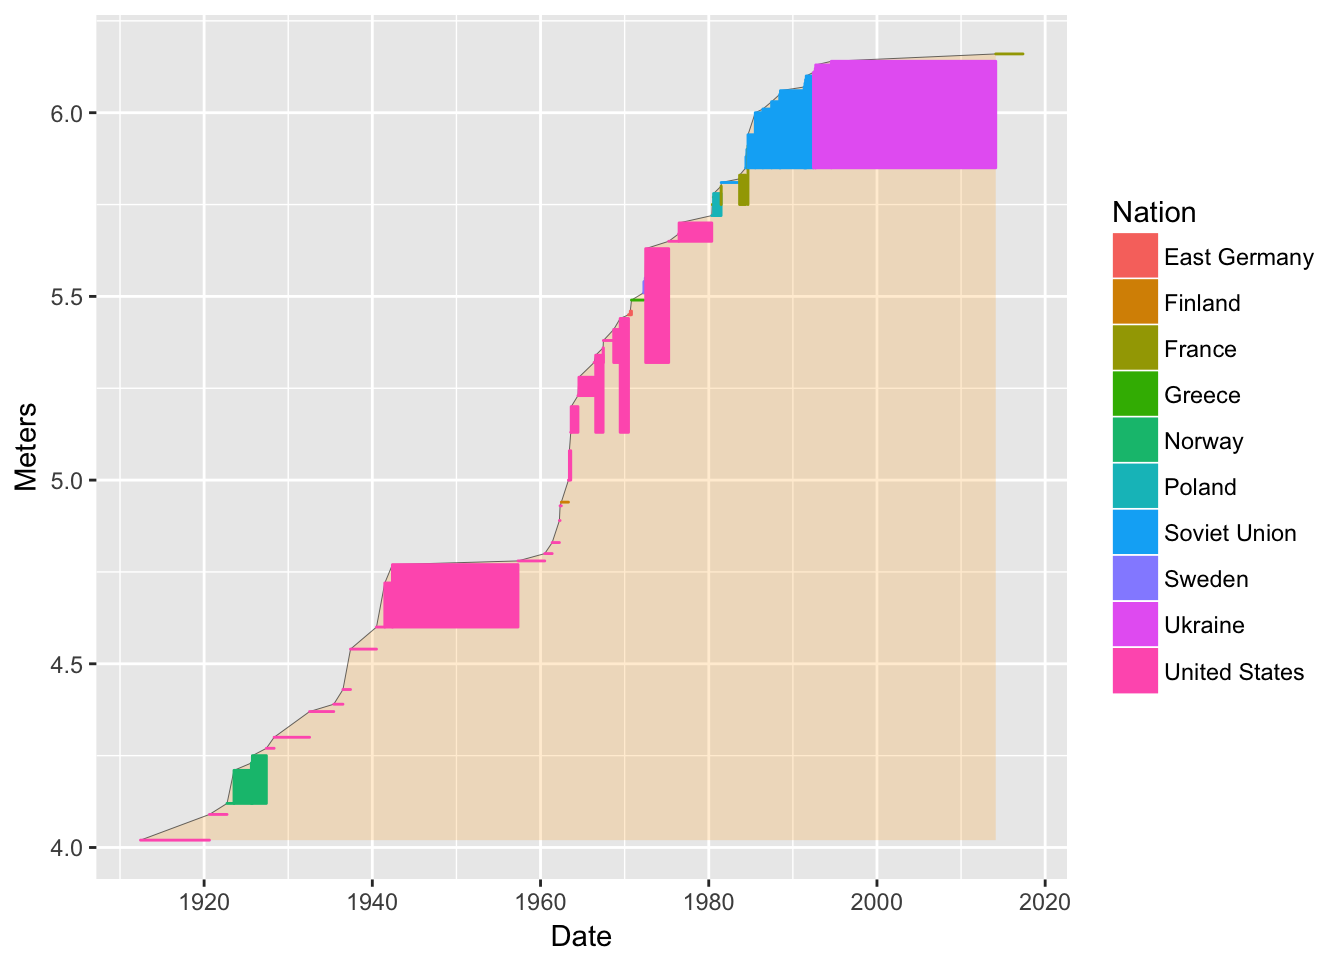
\includegraphics{bookdown-demo_files/figure-latex/unnamed-chunk-51-1.pdf}

I used \texttt{geom\_rect()} to plot rectangles where the bottom edge is
situated at the athlete's lowest world record. Note how it required
massaging some data into the data frame at the beginning.

\subsection{More! Add some text to it!}\label{more-add-some-text-to-it}

Now, I want to try to get every single name in the first time the person
set the record. Of course, they won't all fit exactly at the point (Date
and Meters) of each record, so let's space them out evenly, then draw
little line segments to meet up with the records.

\begin{enumerate}
\def\labelenumi{\arabic{enumi}.}
\item
  We make a new data frame that has just the first time a person got a
  record

\begin{Shaded}
\begin{Highlighting}[]
\NormalTok{pv1 <-}\StringTok{ }\NormalTok{pv %>%}\StringTok{ }
\StringTok{  }\KeywordTok{filter}\NormalTok{(}\StringTok{`}\DataTypeTok{#[2]}\StringTok{`} \NormalTok{==}\StringTok{ }\DecValTok{1}\NormalTok{)}
\NormalTok{pv1 }\CommentTok{# have a look at it}
\end{Highlighting}
\end{Shaded}

\begin{verbatim}
## # A tibble: 34 × 9
##    Record        Athlete        Nation                       Venue
##     <chr>          <chr>         <chr>                       <chr>
## 1  4.02 m    Marc Wright United States             Cambridge, U.S.
## 2  4.09 m     Frank Foss United States            Antwerp, Belgium
## 3  4.12 m   Charles Hoff        Norway         Copenhagen, Denmark
## 4  4.27 m     Sabin Carr United States          Philadelphia, U.S.
## 5  4.30 m     Lee Barnes United States                Fresno, U.S.
## 6  4.37 m William Graber United States             Palo Alto, U.S.
## 7  4.39 m    Keith Brown United States                Boston, U.S.
## 8  4.43 m  George Varoff United States Princeton, New Jersey, U.S.
## 9  4.54 m    Bill Sefton United States           Los Angeles, U.S.
## 10 4.54 m  Earle Meadows United States           Los Angeles, U.S.
## # ... with 24 more rows, and 5 more variables: Date <date>, `#[2]` <int>,
## #   Meters <dbl>, FirstRecordMeters <dbl>, DateNext <date>
\end{verbatim}
\item
  Look at the previous plot and decide that we would like to run names
  equally spaced along a line that runs from about (1910, 4.25) to
  (1980, 6.5). Note that we will have to squish 34 names along that
  line. So, we can define the points along it as follows:

\begin{Shaded}
\begin{Highlighting}[]
\NormalTok{pv1 <-}\StringTok{ }\NormalTok{pv1 %>%}
\StringTok{  }\KeywordTok{mutate}\NormalTok{(}\DataTypeTok{nameline.x =} \KeywordTok{seq}\NormalTok{(}\KeywordTok{mdy}\NormalTok{(}\StringTok{"1-1-1910"}\NormalTok{), }\KeywordTok{mdy}\NormalTok{(}\StringTok{"1-1-1980"}\NormalTok{), }\DataTypeTok{length.out =} \KeywordTok{nrow}\NormalTok{(.)),}
         \DataTypeTok{nameline.y =} \KeywordTok{seq}\NormalTok{(}\FloatTok{4.5}\NormalTok{, }\FloatTok{6.44}\NormalTok{, }\DataTypeTok{length.out =} \KeywordTok{nrow}\NormalTok{(.)))}

\NormalTok{pv1$nameline.x <-}\StringTok{ }\KeywordTok{seq}\NormalTok{(}\KeywordTok{mdy}\NormalTok{(}\StringTok{"1-1-1910"}\NormalTok{), }\KeywordTok{mdy}\NormalTok{(}\StringTok{"1-1-1980"}\NormalTok{), }\DataTypeTok{length.out =} \KeywordTok{nrow}\NormalTok{(pv1))}
\CommentTok{# holy cow! did you see how easily we got that sequence of dates? lubridate is amazing!}
\NormalTok{pv1$nameline.y <-}\StringTok{ }\KeywordTok{seq}\NormalTok{(}\FloatTok{4.5}\NormalTok{, }\FloatTok{6.44}\NormalTok{, }\DataTypeTok{length.out =} \KeywordTok{nrow}\NormalTok{(pv1))}
\end{Highlighting}
\end{Shaded}
\item
  Add that line to the plot as colored points atop a black line.

\begin{Shaded}
\begin{Highlighting}[]
\NormalTok{bb2 <-}\StringTok{ }\NormalTok{bb +}\StringTok{ }
\StringTok{  }\KeywordTok{geom_line}\NormalTok{(}\DataTypeTok{data =} \NormalTok{pv1, }\DataTypeTok{mapping =} \KeywordTok{aes}\NormalTok{(}\DataTypeTok{x =} \NormalTok{nameline.x, }\DataTypeTok{y =} \NormalTok{nameline.y), }\DataTypeTok{color =} \StringTok{"black"}\NormalTok{, }\DataTypeTok{size =} \FloatTok{0.2}\NormalTok{) +}
\StringTok{  }\KeywordTok{geom_point}\NormalTok{(}\DataTypeTok{data =} \NormalTok{pv1, }\DataTypeTok{mapping =} \KeywordTok{aes}\NormalTok{(}\DataTypeTok{x =} \NormalTok{nameline.x, }\DataTypeTok{y =} \NormalTok{nameline.y))}
\NormalTok{bb2}
\end{Highlighting}
\end{Shaded}

  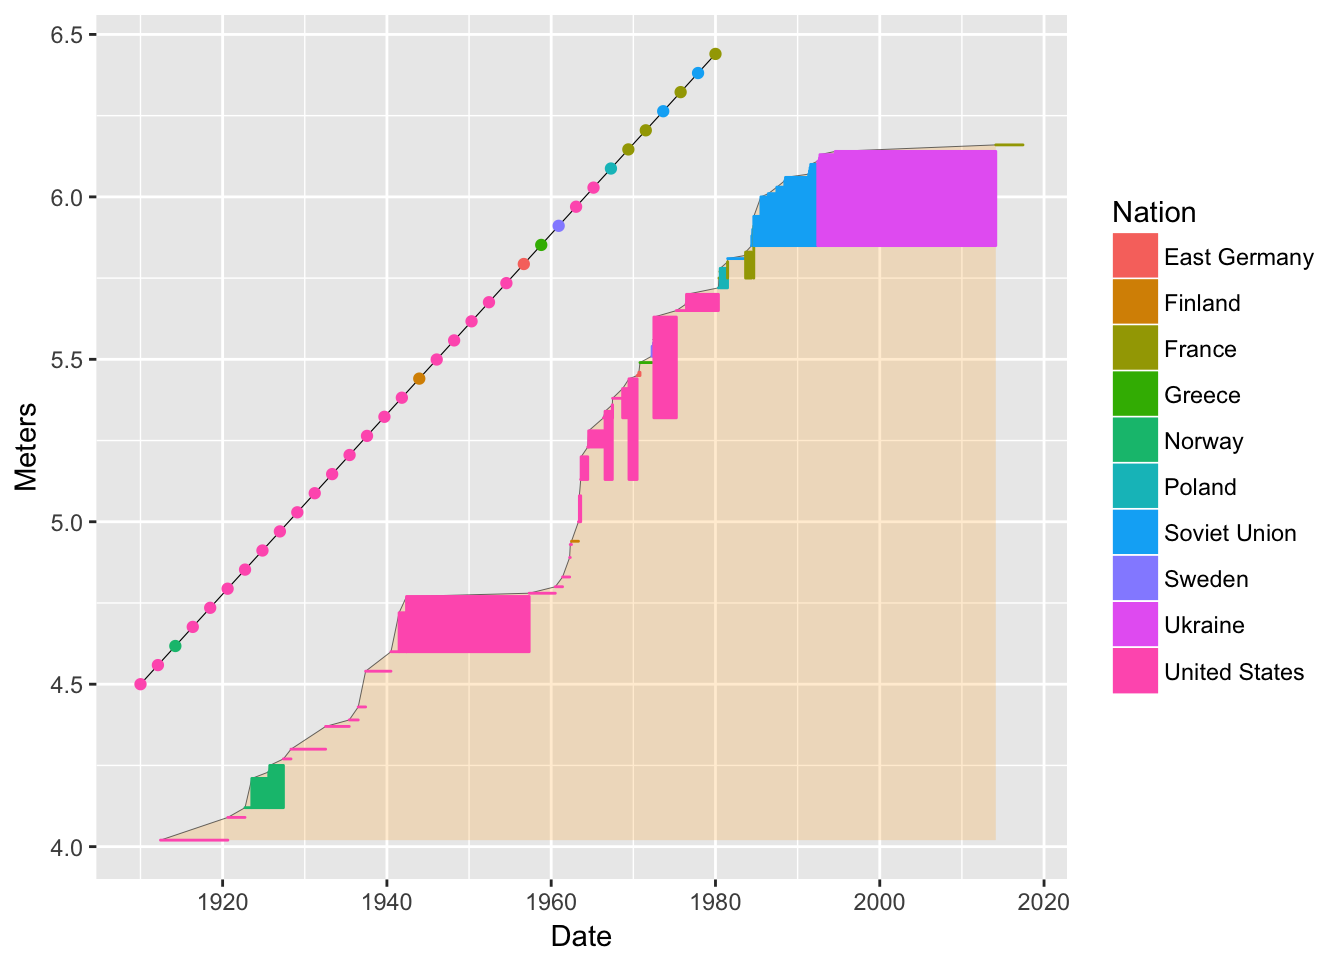
\includegraphics{bookdown-demo_files/figure-latex/unnamed-chunk-54-1.pdf}

  Notice how the color of Nation gets applied to the points
  automatically.
\item
  Now, little colored lines from the nameline points to the records. For
  this we can use the \texttt{geom\_segment()} function.

\begin{Shaded}
\begin{Highlighting}[]
\NormalTok{bb3 <-}\StringTok{ }\NormalTok{bb2 +}\StringTok{ }\KeywordTok{geom_segment}\NormalTok{(}\DataTypeTok{data =} \NormalTok{pv1, }\DataTypeTok{mapping =} \KeywordTok{aes}\NormalTok{(}\DataTypeTok{xend =} \NormalTok{nameline.x, }\DataTypeTok{yend =} \NormalTok{nameline.y))}
\NormalTok{bb3}
\end{Highlighting}
\end{Shaded}

  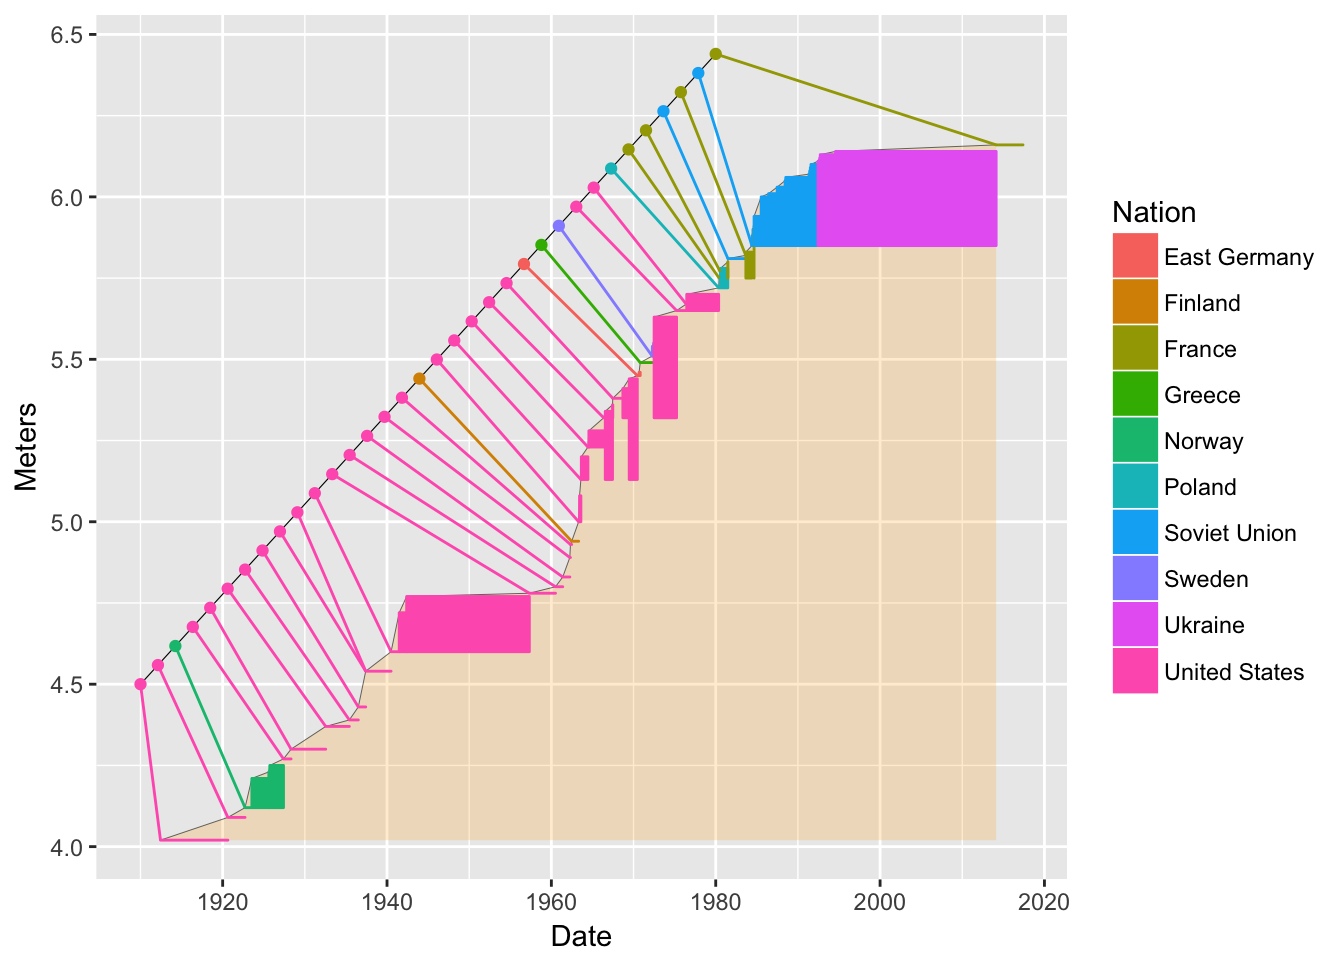
\includegraphics{bookdown-demo_files/figure-latex/unnamed-chunk-55-1.pdf}
\item
  Finally, we want to add the names of the athletes in there. We already
  have their names in \texttt{pv1}. We use the \texttt{geom\_text()}
  function.

\begin{Shaded}
\begin{Highlighting}[]
\NormalTok{bb4 <-}\StringTok{ }\NormalTok{bb3 +}\StringTok{ }\KeywordTok{geom_text}\NormalTok{(}\DataTypeTok{data =} \NormalTok{pv1, }
                       \KeywordTok{aes}\NormalTok{(}\DataTypeTok{label =} \NormalTok{Athlete, }
                           \DataTypeTok{x =} \NormalTok{nameline.x, }
                           \DataTypeTok{y =} \NormalTok{nameline.y +}\StringTok{ }\NormalTok{.}\DecValTok{05}\NormalTok{), }
                       \DataTypeTok{angle =} \NormalTok{-}\DecValTok{45}\NormalTok{, }\DataTypeTok{hjust =} \DecValTok{1}\NormalTok{)}
\NormalTok{bb4}
\end{Highlighting}
\end{Shaded}

  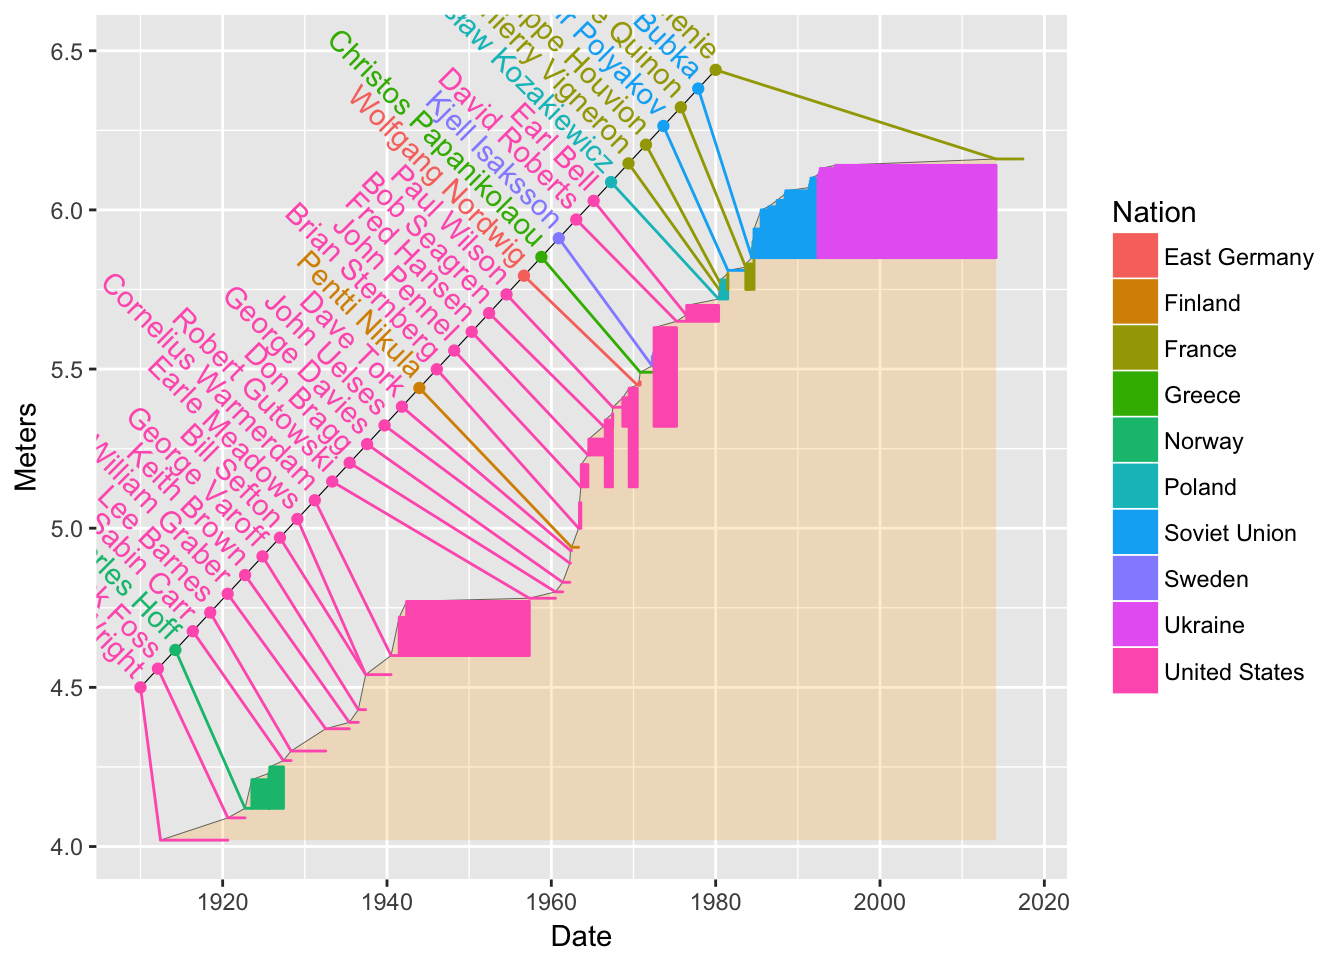
\includegraphics{bookdown-demo_files/figure-latex/unnamed-chunk-56-1.pdf}
\item
  That is pretty cool, but a lot of names have gotten chopped off. Can
  we do something about that? There might be something a little more
  automatic, but we can do it by-hand, too:

\begin{Shaded}
\begin{Highlighting}[]
\NormalTok{bb4 +}\StringTok{ }\KeywordTok{coord_cartesian}\NormalTok{(}\DataTypeTok{xlim =} \KeywordTok{mdy}\NormalTok{(}\KeywordTok{c}\NormalTok{(}\StringTok{"1-1-1898"}\NormalTok{, }\StringTok{"1-1-2020"}\NormalTok{)), }\DataTypeTok{ylim =} \KeywordTok{c}\NormalTok{(}\FloatTok{3.8}\NormalTok{, }\FloatTok{7.1}\NormalTok{))}
\end{Highlighting}
\end{Shaded}

  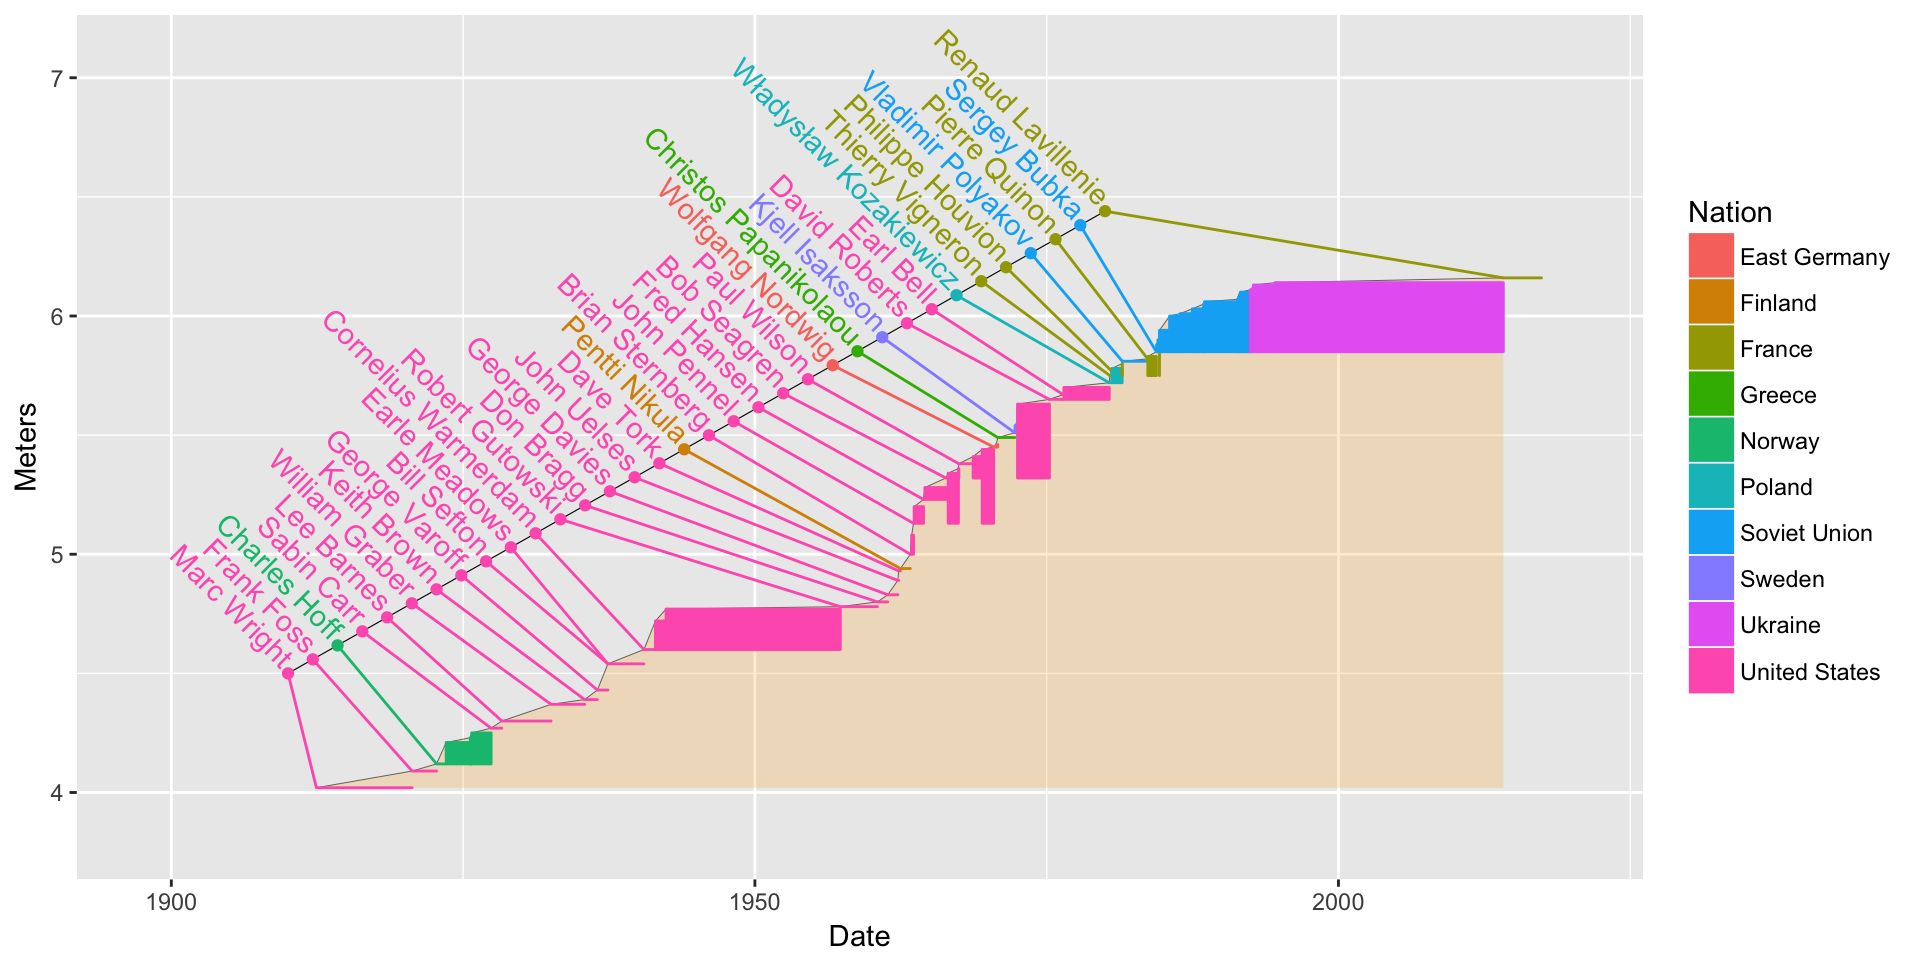
\includegraphics{bookdown-demo_files/figure-latex/unnamed-chunk-57-1.pdf}
\end{enumerate}

\chapter{Making Maps with R}\label{map-making-in-R}

\section{Intro}\label{map-making-intro}

For a long time, R has had a relatively simple mechanism, via the
\texttt{maps} package, for making simple outlines of maps and plotting
lat-long points and paths on them.

More recently, with the advent of packages like \texttt{sp},
\texttt{rgdal}, and \texttt{rgeos}, R has been acquiring much of the
functionality of traditional GIS packages (like ArcGIS, etc). This is an
exciting development, but not always easily accessible for the beginner,
as it requires installation of specialized external libraries (that may,
on some platforms, not be straightforward) and considerable familiarity
with GIS concepts.

More recently, a third approach to convenient mapping, using
\texttt{ggmap} has been developed that allows the tiling of detailed
base maps from Google Earth or Open Street Maps, upon which spatial data
may be plotted. Today, we are going to focus on mapping using base maps
from R's tried and true \texttt{maps} package and also using the
\texttt{ggmap} package. We won't cover the more advanced GIS-related
topics nor using \texttt{rgdal}, or \texttt{sp} to plot maps with
different projections, etc. Nor will cover the somewhat more simplified
approach to projections using the \texttt{mapproj} package.

As in our previous explorations in this course, when it comes to
plotting, we are going to completely skip over R's base graphics system
and head directly to Hadley Wickham's \texttt{ggplot2} package. Hadley
has included a few functions that make it relatively easy to interact
with the data in R's \texttt{maps} package, and of course, once a map
layer is laid down, you have all the power of ggplot at your fingertips
to overlay whatever you may want to over the map. \texttt{ggmap} is a
package that goes out to different map servers and grabs base maps to
plot things on, then it sets up the coordinate system and writes it out
as the base layer for further ggplotting. It is pretty sweet, but does
not support different projections.

\subsection{Today's Goals}\label{todays-goals}

\begin{enumerate}
\def\labelenumi{\arabic{enumi}.}
\tightlist
\item
  Introduce readers to the map outlines available in the \texttt{maps}
  package

  \begin{itemize}
  \tightlist
  \item
    Show how to convert those data into data frames that
    \texttt{ggplot2} can deal with
  \item
    Discuss some \texttt{ggplot2} related issues about plotting things.
  \end{itemize}
\item
  Use \texttt{ggmap} to make some pretty decent looking maps
\end{enumerate}

I feel that the above twp topics should cover a large part of what
people will need for making useful maps of field sites, or sampling
locations, or fishing track lines, etc.

For today we will be skipping how to read in traditional GIS
``shapefiles'' so as to minimize the number of packages that need
installation, but keep in mind that it isn't too hard to do that in R,
too.

\subsection{Prerequisites}\label{prerequisites}

You are going to need to install a few extra packages to follow along
with this lecture.

\begin{Shaded}
\begin{Highlighting}[]
\CommentTok{# these are packages you will need, but probably already have.}
\CommentTok{# Don't bother installing if you already have them}
\KeywordTok{install.packages}\NormalTok{(}\KeywordTok{c}\NormalTok{(}\StringTok{"ggplot2"}\NormalTok{, }\StringTok{"devtools"}\NormalTok{, }\StringTok{"dplyr"}\NormalTok{, }\StringTok{"stringr"}\NormalTok{))}

\CommentTok{# some standard map packages.}
\KeywordTok{install.packages}\NormalTok{(}\KeywordTok{c}\NormalTok{(}\StringTok{"maps"}\NormalTok{, }\StringTok{"mapdata"}\NormalTok{))}

\CommentTok{# the github version of ggmap, which recently pulled in a small fix I had}
\CommentTok{# for a bug }
\NormalTok{devtools::}\KeywordTok{install_github}\NormalTok{(}\StringTok{"dkahle/ggmap"}\NormalTok{)}
\end{Highlighting}
\end{Shaded}

\subsection{Load up a few of the libraries we will
use}\label{load-up-a-few-of-the-libraries-we-will-use}

\begin{Shaded}
\begin{Highlighting}[]
\KeywordTok{library}\NormalTok{(tidyverse)}
\KeywordTok{library}\NormalTok{(mapdata)}
\KeywordTok{library}\NormalTok{(maps)}
\end{Highlighting}
\end{Shaded}

\section{Plotting maps-package maps with
ggplot}\label{maps-package-and-ggplot}

\subsection{The main players:}\label{the-main-players}

\begin{itemize}
\tightlist
\item
  The \texttt{maps} package contains a lot of outlines of continents,
  countries, states, and counties that have been with R for a long
  time.\\
\item
  The \texttt{mapdata} package contains a few more, higher-resolution
  outlines.
\item
  The \texttt{maps} package comes with a plotting function, but, we will
  opt to use \texttt{ggplot2} to plot the maps in the \texttt{maps}
  package.\\
\item
  Recall that \texttt{ggplot2} operates on data frames. Therefore we
  need some way to translate the \texttt{maps} data into a data frame
  format the \texttt{ggplot} can use.
\end{itemize}

\subsection{Maps in the maps package}\label{maps-in-the-maps-package}

\begin{itemize}
\tightlist
\item
  Package \texttt{maps} provides lots of different map outlines and
  points for cities, etc.\\
\item
  Some examples: \texttt{usa}, \texttt{nz}, \texttt{state},
  \texttt{world}, etc.
\end{itemize}

\subsection{Makin' data frames from map
outlines}\label{makin-data-frames-from-map-outlines}

\begin{itemize}
\item
  \texttt{ggplot2} provides the \texttt{map\_data()} function.

  \begin{itemize}
  \tightlist
  \item
    Think of it as a function that turns a series of points along an
    outline into a data frame of those points.
  \item
    Syntax: \texttt{map\_data("name")} where ``name'' is a quoted string
    of the name of a map in the \texttt{maps} or \texttt{mapdata}
    package
  \end{itemize}
\item
  Here we get a USA map from \texttt{maps}:

\begin{Shaded}
\begin{Highlighting}[]
\NormalTok{usa <-}\StringTok{ }\KeywordTok{map_data}\NormalTok{(}\StringTok{"usa"}\NormalTok{)}

\KeywordTok{dim}\NormalTok{(usa)}
\end{Highlighting}
\end{Shaded}

\begin{verbatim}
## [1] 7243    6
\end{verbatim}

\begin{Shaded}
\begin{Highlighting}[]
\KeywordTok{head}\NormalTok{(usa)}
\end{Highlighting}
\end{Shaded}

\begin{verbatim}
##        long      lat group order region subregion
## 1 -101.4078 29.74224     1     1   main      <NA>
## 2 -101.3906 29.74224     1     2   main      <NA>
## 3 -101.3620 29.65056     1     3   main      <NA>
## 4 -101.3505 29.63911     1     4   main      <NA>
## 5 -101.3219 29.63338     1     5   main      <NA>
## 6 -101.3047 29.64484     1     6   main      <NA>
\end{verbatim}

\begin{Shaded}
\begin{Highlighting}[]
\KeywordTok{tail}\NormalTok{(usa)}
\end{Highlighting}
\end{Shaded}

\begin{verbatim}
##           long      lat group order         region subregion
## 7247 -122.6187 48.37482    10  7247 whidbey island      <NA>
## 7248 -122.6359 48.35764    10  7248 whidbey island      <NA>
## 7249 -122.6703 48.31180    10  7249 whidbey island      <NA>
## 7250 -122.7218 48.23732    10  7250 whidbey island      <NA>
## 7251 -122.7104 48.21440    10  7251 whidbey island      <NA>
## 7252 -122.6703 48.17429    10  7252 whidbey island      <NA>
\end{verbatim}
\item
  Here is the high-res world map centered on the Pacific Ocean from
  \texttt{mapdata}

\begin{Shaded}
\begin{Highlighting}[]
\NormalTok{w2hr <-}\StringTok{ }\KeywordTok{map_data}\NormalTok{(}\StringTok{"world2Hires"}\NormalTok{)}

\KeywordTok{dim}\NormalTok{(w2hr)}
\end{Highlighting}
\end{Shaded}

\begin{verbatim}
## [1] 2274539       6
\end{verbatim}

\begin{Shaded}
\begin{Highlighting}[]
\KeywordTok{head}\NormalTok{(w2hr)}
\end{Highlighting}
\end{Shaded}

\begin{verbatim}
##       long      lat group order region subregion
## 1 226.6336 58.42416     1     1 Canada      <NA>
## 2 226.6314 58.42336     1     2 Canada      <NA>
## 3 226.6122 58.41196     1     3 Canada      <NA>
## 4 226.5911 58.40027     1     4 Canada      <NA>
## 5 226.5719 58.38864     1     5 Canada      <NA>
## 6 226.5528 58.37724     1     6 Canada      <NA>
\end{verbatim}

\begin{Shaded}
\begin{Highlighting}[]
\KeywordTok{tail}\NormalTok{(w2hr)}
\end{Highlighting}
\end{Shaded}

\begin{verbatim}
##             long      lat group   order      region subregion
## 2276817 125.0258 11.18471  2284 2276817 Philippines     Leyte
## 2276818 125.0172 11.17142  2284 2276818 Philippines     Leyte
## 2276819 125.0114 11.16110  2284 2276819 Philippines     Leyte
## 2276820 125.0100 11.15555  2284 2276820 Philippines     Leyte
## 2276821 125.0111 11.14861  2284 2276821 Philippines     Leyte
## 2276822 125.0155 11.13887  2284 2276822 Philippines     Leyte
\end{verbatim}
\end{itemize}

\subsection{The structure of those data
frames}\label{the-structure-of-those-data-frames}

These are pretty straightforward:

\begin{itemize}
\tightlist
\item
  \texttt{long} is longitude. Things to the west of the prime meridian
  are negative.
\item
  \texttt{lat} is latitude.
\item
  \texttt{order}. This just shows in which order \texttt{ggplot} should
  ``connect the dots''
\item
  \texttt{region} and \texttt{subregion} tell what region or subregion a
  set of points surrounds.
\item
  \texttt{group}. This is \emph{very important}! \texttt{ggplot2}'s
  functions can take a group argument which controls (amongst other
  things) whether adjacent points should be connected by lines. If they
  are in the same group, then they get connected, but if they are in
  different groups then they don't.

  \begin{itemize}
  \tightlist
  \item
    Essentially, having to points in different groups means that
    \texttt{ggplot} ``lifts the pen'' when going between them.
  \end{itemize}
\end{itemize}

\subsection{Plot the USA map}\label{plot-the-usa-map}

\begin{itemize}
\tightlist
\item
  Maps in this format can be plotted with the polygon geom. i.e.~using
  \texttt{geom\_polygon()}.
\item
  \texttt{geom\_polygon()} drawn lines between points and ``closes them
  up'' (i.e.~draws a line from the last point back to the first point)
\item
  You have to map the \texttt{group} aesthetic to the \texttt{group}
  column
\item
  Of course, \texttt{x\ =\ long} and \texttt{y\ =\ lat} are the other
  aesthetics.
\end{itemize}

\subsubsection{Simple black map}\label{simple-black-map}

By default, \texttt{geom\_polygon()} draws with no line color, but with
a black fill:

\begin{Shaded}
\begin{Highlighting}[]
\NormalTok{usa <-}\StringTok{ }\KeywordTok{map_data}\NormalTok{(}\StringTok{"usa"}\NormalTok{) }\CommentTok{# we already did this, but we can do it again}
\KeywordTok{ggplot}\NormalTok{() +}\StringTok{ }\KeywordTok{geom_polygon}\NormalTok{(}\DataTypeTok{data =} \NormalTok{usa, }\KeywordTok{aes}\NormalTok{(}\DataTypeTok{x=}\NormalTok{long, }\DataTypeTok{y =} \NormalTok{lat, }\DataTypeTok{group =} \NormalTok{group)) +}\StringTok{ }
\StringTok{  }\KeywordTok{coord_quickmap}\NormalTok{()}
\end{Highlighting}
\end{Shaded}

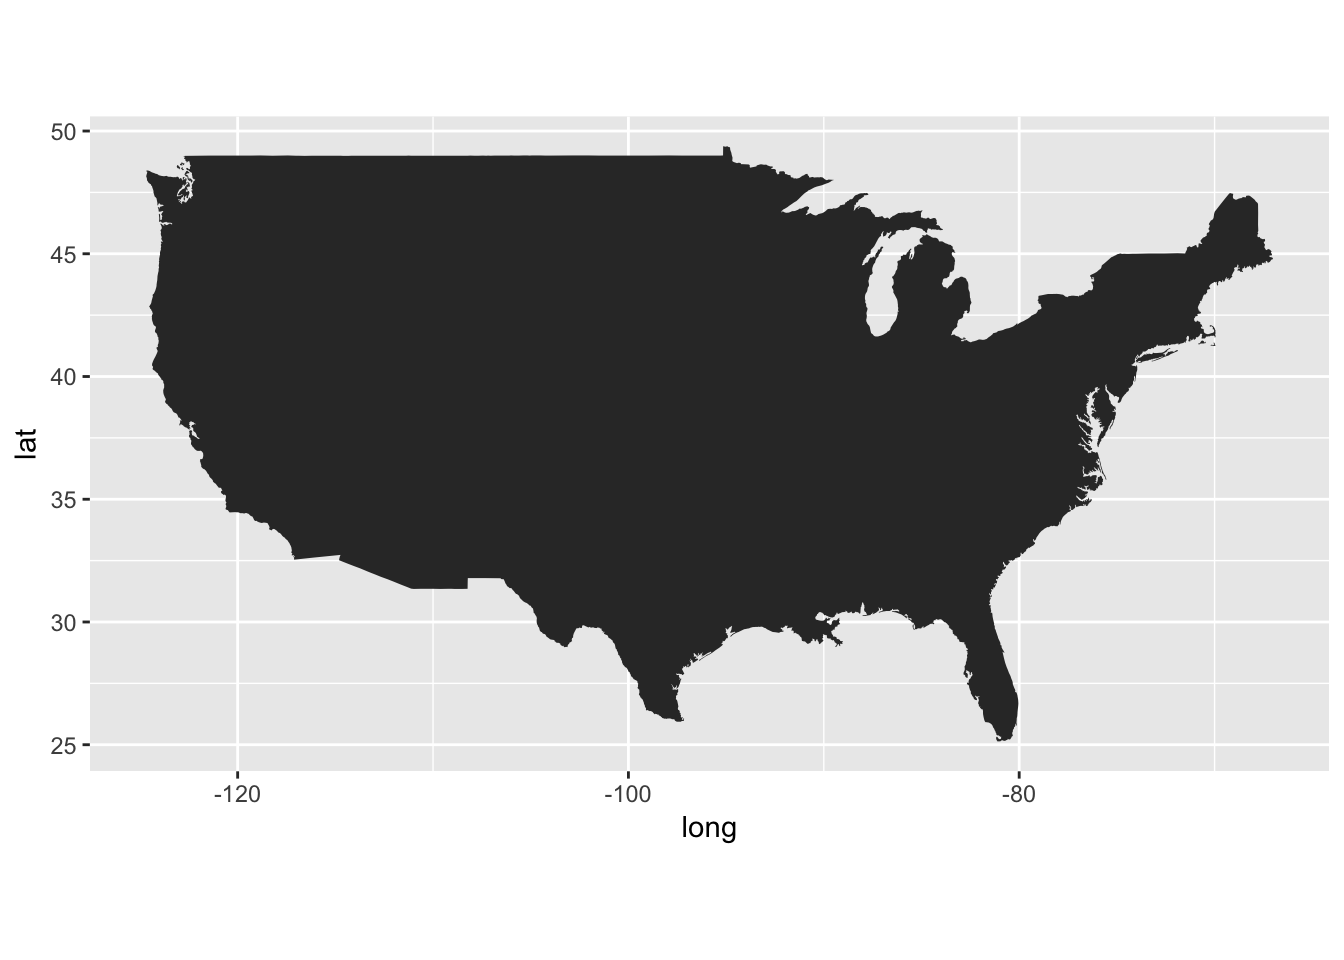
\includegraphics{bookdown-demo_files/figure-latex/unnamed-chunk-62-1.pdf}

\subsubsection{What is this
coord\_quickmap()?}\label{what-is-this-coord_quickmap}

\begin{itemize}
\tightlist
\item
  This is very important when drawing maps.
\item
  It sets the relationship between one unit in the \(y\) direction and
  one unit in the \(x\) direction so that the \emph{aspect ratio} is
  good for your map.
\item
  Then, even if you change the outer dimensions of the plot (i.e.~by
  changing the window size or the size of the pdf file you are saving it
  to (in \texttt{ggsave} for example)), the aspect ratio remains
  unchanged.
\end{itemize}

\subsubsection{Mess with line and fill
colors}\label{mess-with-line-and-fill-colors}

\begin{itemize}
\item
  Here is no fill, with a red line. Remember, fixed value of aesthetics
  go \emph{outside} the \texttt{aes} function.

\begin{Shaded}
\begin{Highlighting}[]
\KeywordTok{ggplot}\NormalTok{() +}\StringTok{ }
\StringTok{  }\KeywordTok{geom_polygon}\NormalTok{(}\DataTypeTok{data =} \NormalTok{usa, }\KeywordTok{aes}\NormalTok{(}\DataTypeTok{x=}\NormalTok{long, }\DataTypeTok{y =} \NormalTok{lat, }\DataTypeTok{group =} \NormalTok{group), }\DataTypeTok{fill =} \OtherTok{NA}\NormalTok{, }\DataTypeTok{color =} \StringTok{"red"}\NormalTok{) +}\StringTok{ }
\StringTok{  }\KeywordTok{coord_quickmap}\NormalTok{()}
\end{Highlighting}
\end{Shaded}

  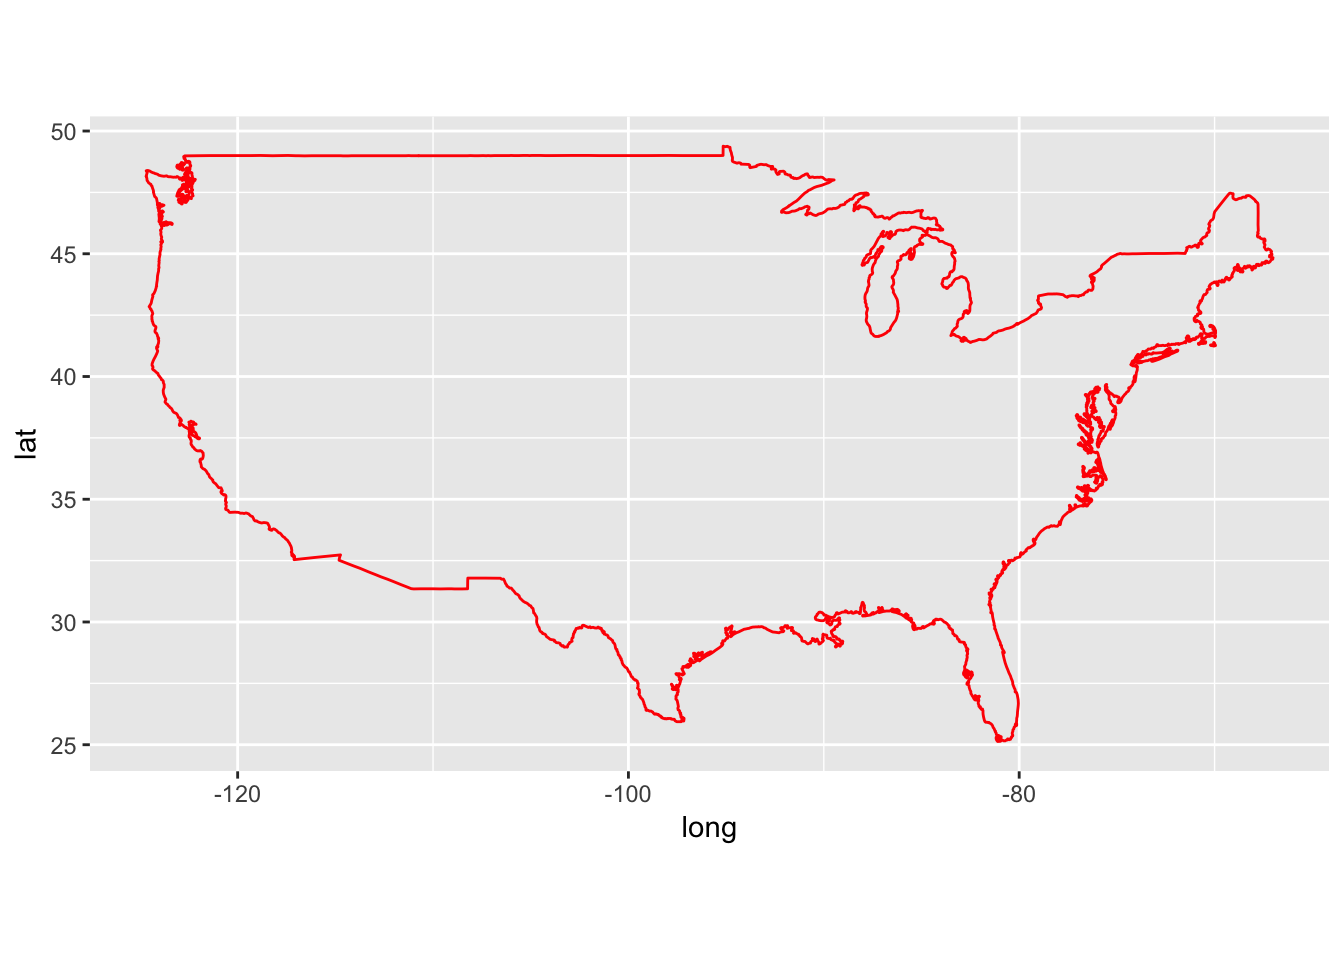
\includegraphics{bookdown-demo_files/figure-latex/unnamed-chunk-63-1.pdf}
\item
  Here is violet fill, with a blue line.

\begin{Shaded}
\begin{Highlighting}[]
\NormalTok{gg1 <-}\StringTok{ }\KeywordTok{ggplot}\NormalTok{() +}\StringTok{ }
\StringTok{  }\KeywordTok{geom_polygon}\NormalTok{(}\DataTypeTok{data =} \NormalTok{usa, }\KeywordTok{aes}\NormalTok{(}\DataTypeTok{x=}\NormalTok{long, }\DataTypeTok{y =} \NormalTok{lat, }\DataTypeTok{group =} \NormalTok{group), }\DataTypeTok{fill =} \StringTok{"violet"}\NormalTok{, }\DataTypeTok{color =} \StringTok{"blue"}\NormalTok{) +}\StringTok{ }
\StringTok{  }\KeywordTok{coord_quickmap}\NormalTok{()}
\NormalTok{gg1}
\end{Highlighting}
\end{Shaded}

  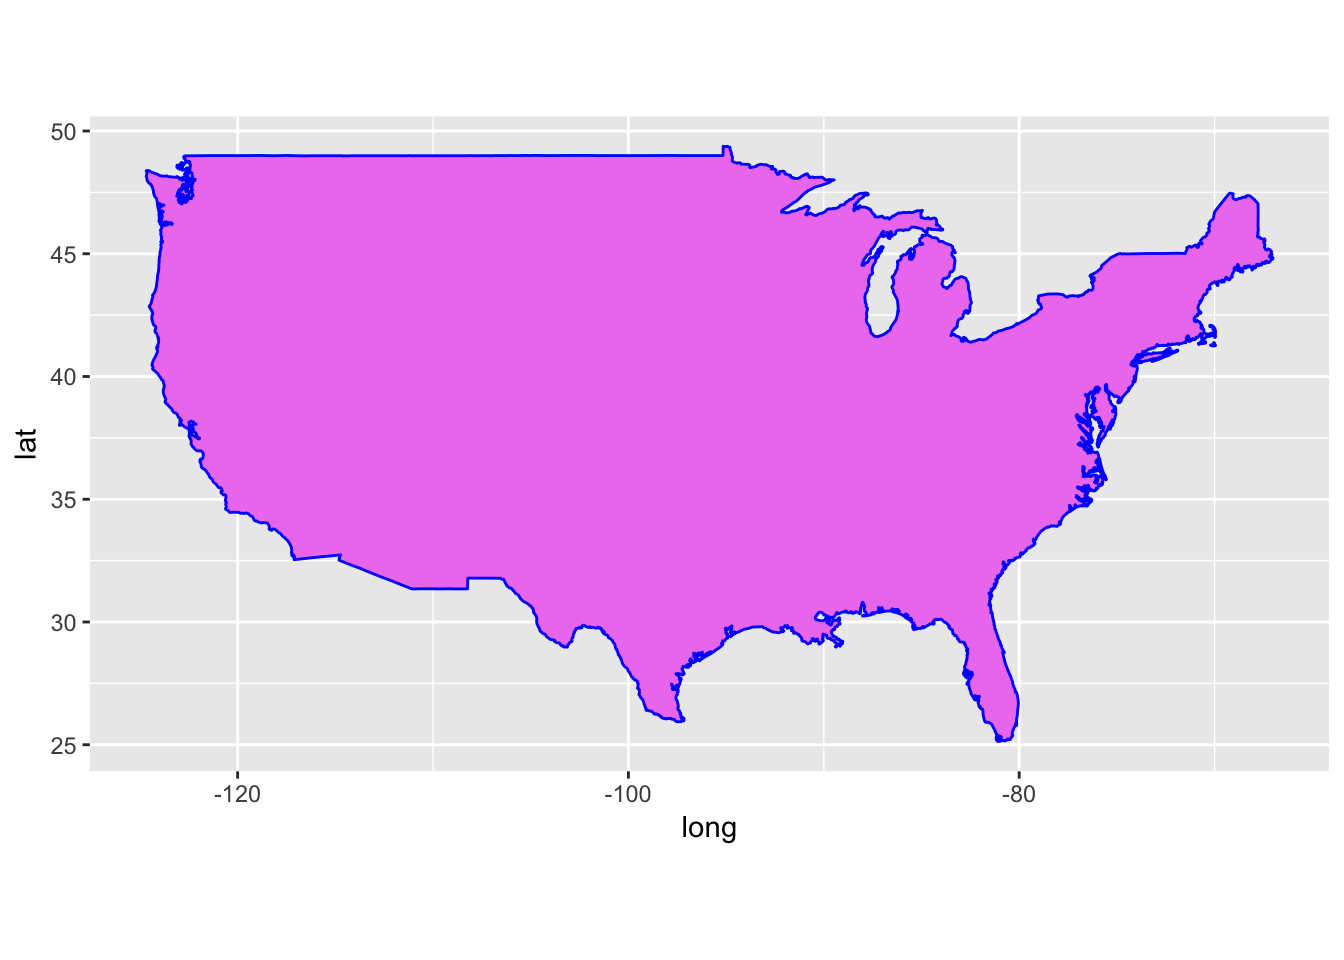
\includegraphics{bookdown-demo_files/figure-latex/unnamed-chunk-64-1.pdf}
\end{itemize}

\subsubsection{Adding points to the map}\label{adding-points-to-the-map}

\begin{itemize}
\item
  Let's add black and yellow points at our lab and at the NWFSC in
  Seattle.

\begin{Shaded}
\begin{Highlighting}[]
\NormalTok{labs <-}\StringTok{ }\KeywordTok{data.frame}\NormalTok{(}
  \DataTypeTok{long =} \KeywordTok{c}\NormalTok{(-}\FloatTok{122.064873}\NormalTok{, -}\FloatTok{122.306417}\NormalTok{),}
  \DataTypeTok{lat =} \KeywordTok{c}\NormalTok{(}\FloatTok{36.951968}\NormalTok{, }\FloatTok{47.644855}\NormalTok{),}
  \DataTypeTok{names =} \KeywordTok{c}\NormalTok{(}\StringTok{"SWFSC-FED"}\NormalTok{, }\StringTok{"NWFSC"}\NormalTok{),}
  \DataTypeTok{stringsAsFactors =} \OtherTok{FALSE}
  \NormalTok{)  }

\NormalTok{gg1 +}\StringTok{ }
\StringTok{  }\KeywordTok{geom_point}\NormalTok{(}\DataTypeTok{data =} \NormalTok{labs, }\KeywordTok{aes}\NormalTok{(}\DataTypeTok{x =} \NormalTok{long, }\DataTypeTok{y =} \NormalTok{lat), }\DataTypeTok{color =} \StringTok{"black"}\NormalTok{, }\DataTypeTok{size =} \DecValTok{5}\NormalTok{) +}
\StringTok{  }\KeywordTok{geom_point}\NormalTok{(}\DataTypeTok{data =} \NormalTok{labs, }\KeywordTok{aes}\NormalTok{(}\DataTypeTok{x =} \NormalTok{long, }\DataTypeTok{y =} \NormalTok{lat), }\DataTypeTok{color =} \StringTok{"yellow"}\NormalTok{, }\DataTypeTok{size =} \DecValTok{4}\NormalTok{)}
\end{Highlighting}
\end{Shaded}

  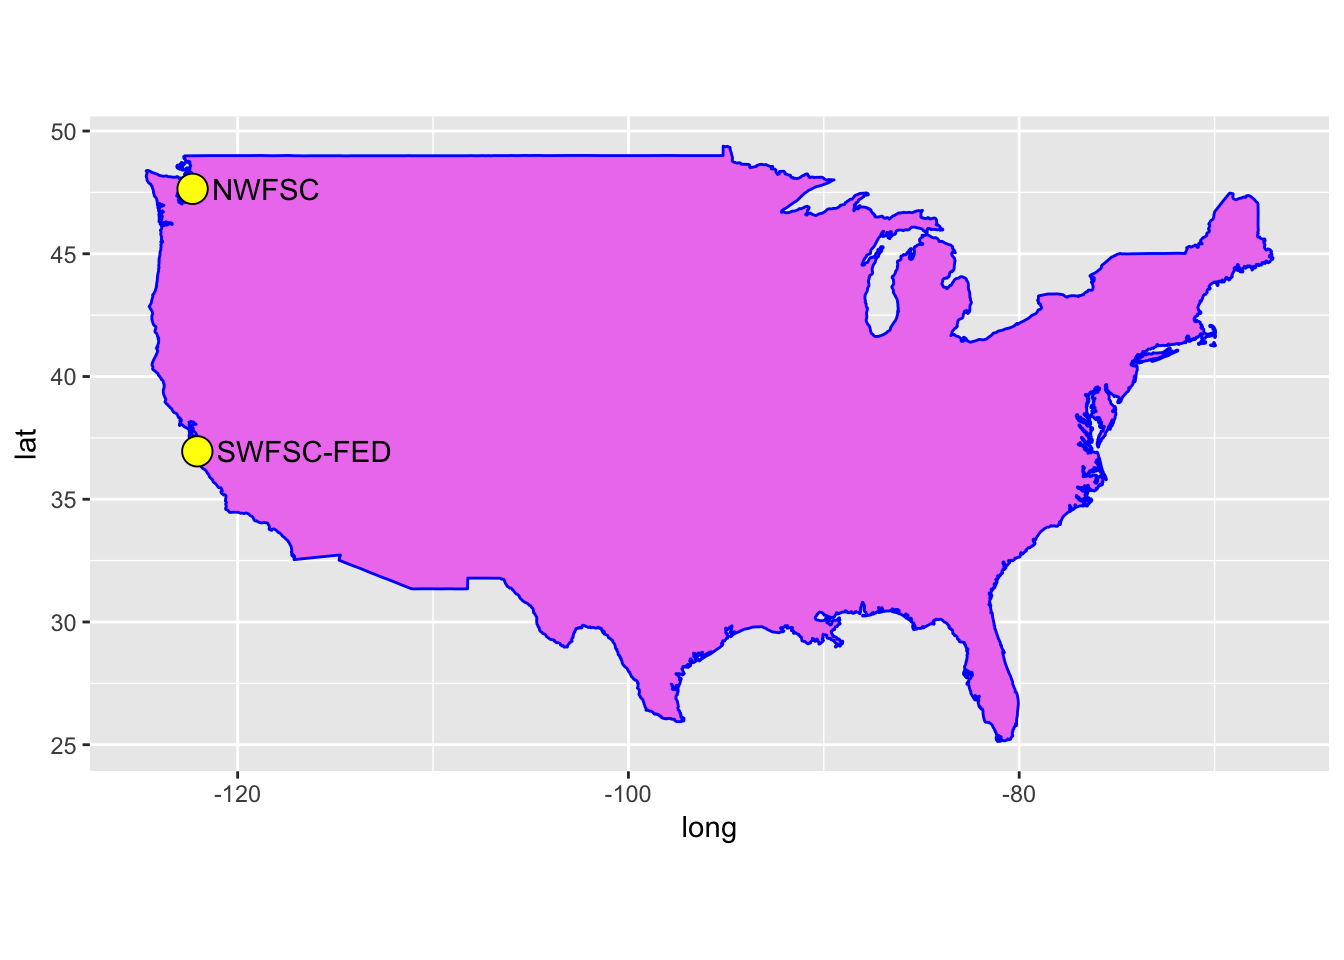
\includegraphics{bookdown-demo_files/figure-latex/unnamed-chunk-65-1.pdf}
\end{itemize}

\subsubsection{See how important the group aesthetic
is}\label{see-how-important-the-group-aesthetic-is}

Here we plot that map without using the group aesthetic:

\begin{Shaded}
\begin{Highlighting}[]
\KeywordTok{ggplot}\NormalTok{() +}\StringTok{ }
\StringTok{      }\KeywordTok{geom_polygon}\NormalTok{(}\DataTypeTok{data =} \NormalTok{usa, }\KeywordTok{aes}\NormalTok{(}\DataTypeTok{x=}\NormalTok{long, }\DataTypeTok{y =} \NormalTok{lat), }\DataTypeTok{fill =} \StringTok{"violet"}\NormalTok{, }\DataTypeTok{color =} \StringTok{"blue"}\NormalTok{) +}\StringTok{ }
\StringTok{      }\KeywordTok{geom_point}\NormalTok{(}\DataTypeTok{data =} \NormalTok{labs, }\KeywordTok{aes}\NormalTok{(}\DataTypeTok{x =} \NormalTok{long, }\DataTypeTok{y =} \NormalTok{lat), }\DataTypeTok{color =} \StringTok{"black"}\NormalTok{, }\DataTypeTok{size =} \DecValTok{5}\NormalTok{) +}
\StringTok{      }\KeywordTok{geom_point}\NormalTok{(}\DataTypeTok{data =} \NormalTok{labs, }\KeywordTok{aes}\NormalTok{(}\DataTypeTok{x =} \NormalTok{long, }\DataTypeTok{y =} \NormalTok{lat), }\DataTypeTok{color =} \StringTok{"yellow"}\NormalTok{, }\DataTypeTok{size =} \DecValTok{4}\NormalTok{) +}
\StringTok{      }\KeywordTok{coord_quickmap}\NormalTok{()}
\end{Highlighting}
\end{Shaded}

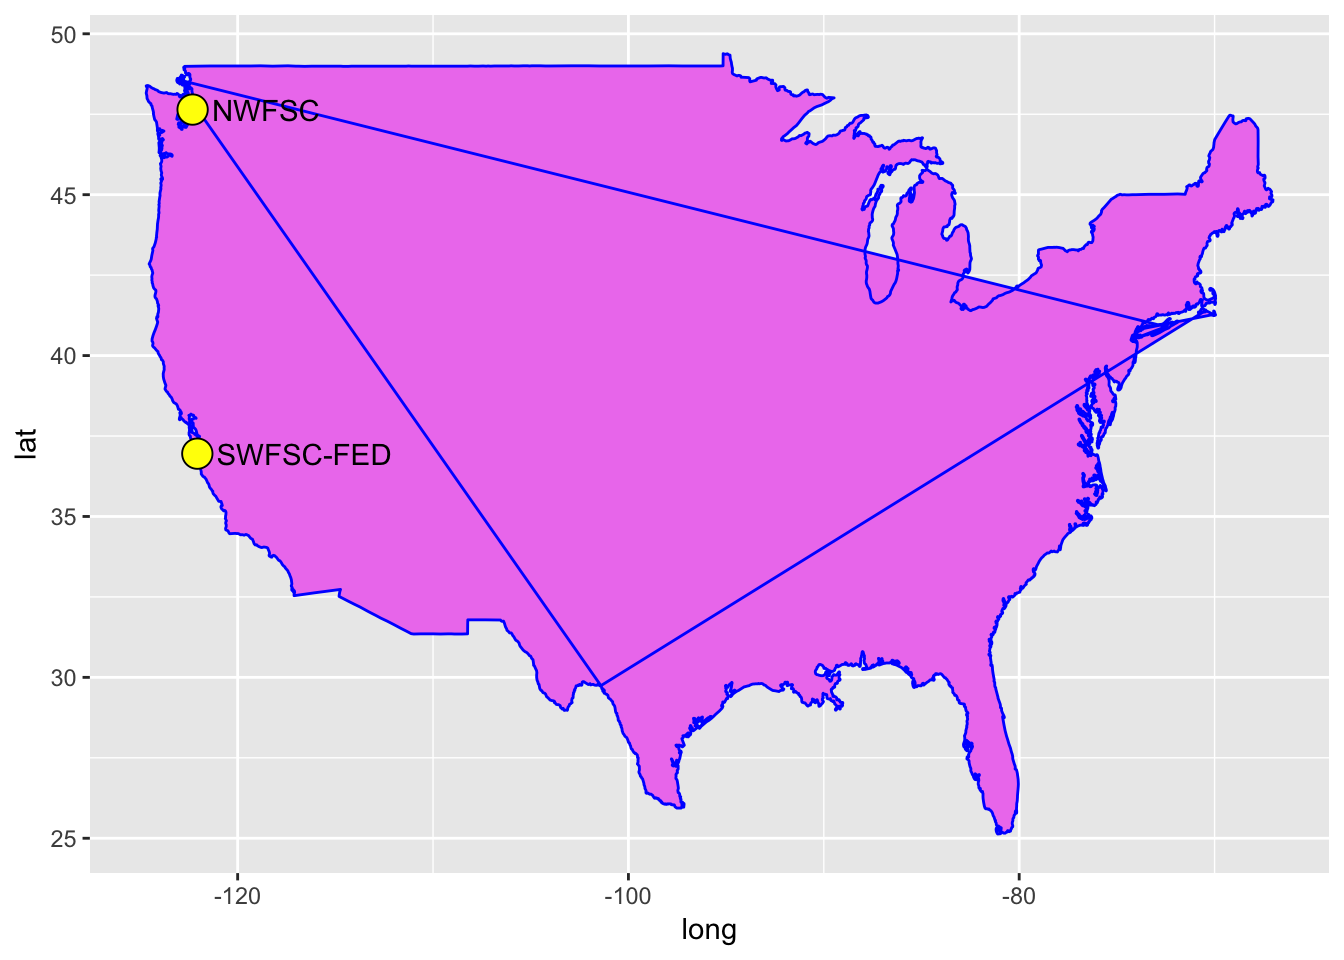
\includegraphics{bookdown-demo_files/figure-latex/unnamed-chunk-66-1.pdf}

That is no bueno! The lines are connecting points that should not be
connected!

\subsection{State maps}\label{state-maps}

We can also get a data frame of polygons that tell us above state
boundaries:

\begin{Shaded}
\begin{Highlighting}[]
\NormalTok{states <-}\StringTok{ }\KeywordTok{map_data}\NormalTok{(}\StringTok{"state"}\NormalTok{)}
\KeywordTok{dim}\NormalTok{(states)}
\end{Highlighting}
\end{Shaded}

\begin{verbatim}
## [1] 15537     6
\end{verbatim}

\begin{Shaded}
\begin{Highlighting}[]
\KeywordTok{head}\NormalTok{(states)}
\end{Highlighting}
\end{Shaded}

\begin{verbatim}
##        long      lat group order  region subregion
## 1 -87.46201 30.38968     1     1 alabama      <NA>
## 2 -87.48493 30.37249     1     2 alabama      <NA>
## 3 -87.52503 30.37249     1     3 alabama      <NA>
## 4 -87.53076 30.33239     1     4 alabama      <NA>
## 5 -87.57087 30.32665     1     5 alabama      <NA>
## 6 -87.58806 30.32665     1     6 alabama      <NA>
\end{verbatim}

\begin{Shaded}
\begin{Highlighting}[]
\KeywordTok{tail}\NormalTok{(states)}
\end{Highlighting}
\end{Shaded}

\begin{verbatim}
##            long      lat group order  region subregion
## 15594 -106.3295 41.00659    63 15594 wyoming      <NA>
## 15595 -106.8566 41.01232    63 15595 wyoming      <NA>
## 15596 -107.3093 41.01805    63 15596 wyoming      <NA>
## 15597 -107.9223 41.01805    63 15597 wyoming      <NA>
## 15598 -109.0568 40.98940    63 15598 wyoming      <NA>
## 15599 -109.0511 40.99513    63 15599 wyoming      <NA>
\end{verbatim}

\subsubsection{Plot all the states, all colored a little
differently}\label{plot-all-the-states-all-colored-a-little-differently}

This is just like it is above, but we can map fill to \texttt{region}
and make sure the the lines of state borders are white.

\begin{Shaded}
\begin{Highlighting}[]
\KeywordTok{ggplot}\NormalTok{(}\DataTypeTok{data =} \NormalTok{states) +}\StringTok{ }
\StringTok{  }\KeywordTok{geom_polygon}\NormalTok{(}\KeywordTok{aes}\NormalTok{(}\DataTypeTok{x =} \NormalTok{long, }\DataTypeTok{y =} \NormalTok{lat, }\DataTypeTok{fill =} \NormalTok{region, }\DataTypeTok{group =} \NormalTok{group), }\DataTypeTok{color =} \StringTok{"white"}\NormalTok{) +}\StringTok{ }
\StringTok{  }\KeywordTok{coord_quickmap}\NormalTok{() +}
\StringTok{  }\KeywordTok{guides}\NormalTok{(}\DataTypeTok{fill=}\OtherTok{FALSE}\NormalTok{)  }\CommentTok{# do this to leave off the color legend}
\end{Highlighting}
\end{Shaded}

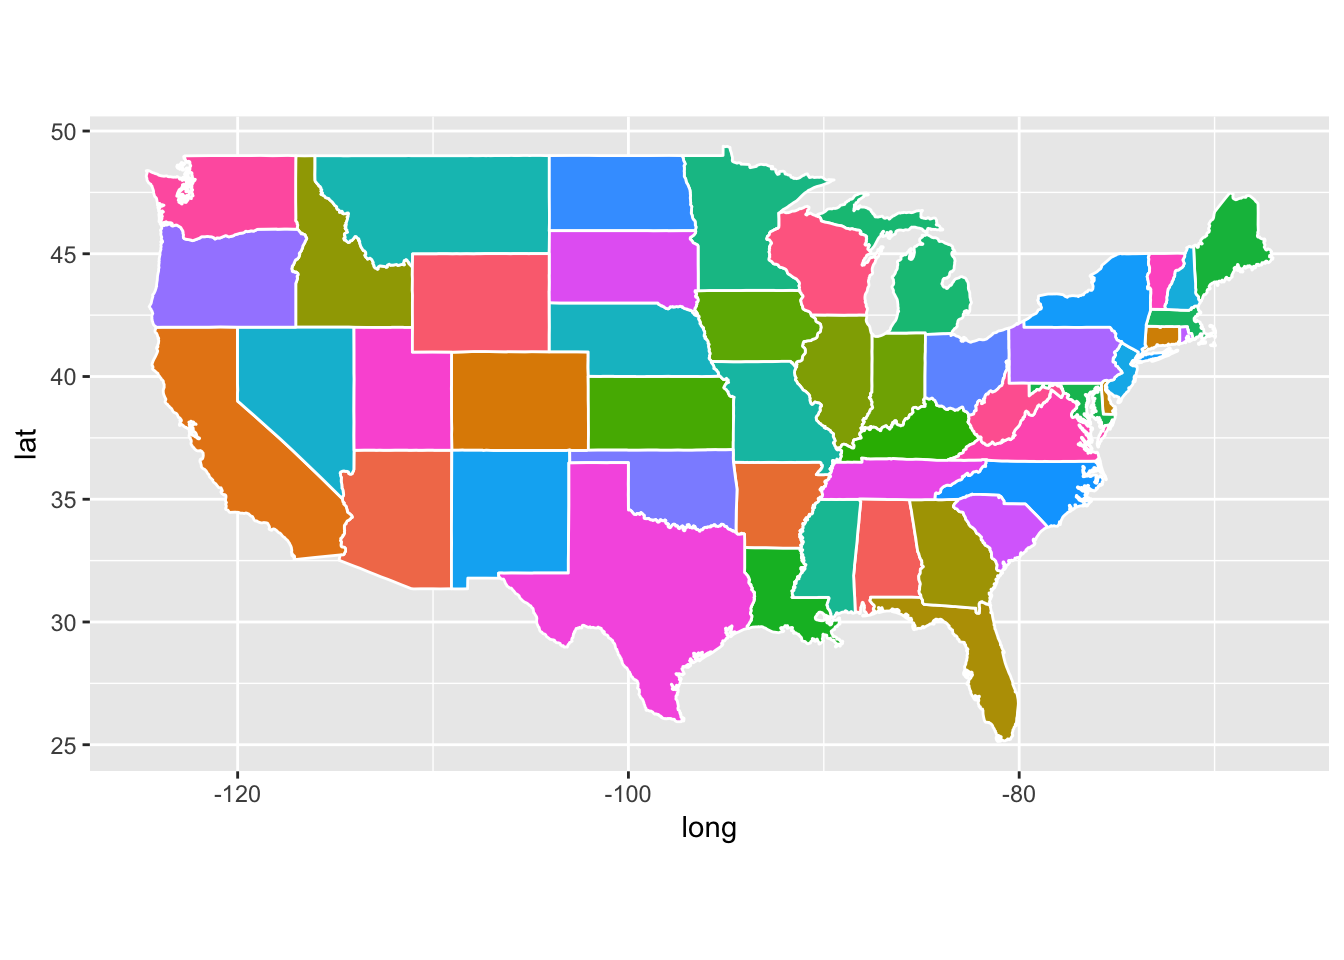
\includegraphics{bookdown-demo_files/figure-latex/unnamed-chunk-68-1.pdf}

Boom! That is easy.

\subsubsection{Plot just a subset of states in the contiguous
48:}\label{plot-just-a-subset-of-states-in-the-contiguous-48}

\begin{itemize}
\item
  Read about the \texttt{subset} command. It provides another way of
  subsetting data frames (sort of like using the \texttt{{[}\ {]}}
  operator with a logical vector).
\item
  We can use it to grab just CA, OR, and WA:

\begin{Shaded}
\begin{Highlighting}[]
\NormalTok{west_coast <-}\StringTok{ }\KeywordTok{subset}\NormalTok{(states, region %in%}\StringTok{ }\KeywordTok{c}\NormalTok{(}\StringTok{"california"}\NormalTok{, }\StringTok{"oregon"}\NormalTok{, }\StringTok{"washington"}\NormalTok{))}

\KeywordTok{ggplot}\NormalTok{(}\DataTypeTok{data =} \NormalTok{west_coast) +}\StringTok{ }
\StringTok{  }\KeywordTok{geom_polygon}\NormalTok{(}\KeywordTok{aes}\NormalTok{(}\DataTypeTok{x =} \NormalTok{long, }\DataTypeTok{y =} \NormalTok{lat), }\DataTypeTok{fill =} \StringTok{"palegreen"}\NormalTok{, }\DataTypeTok{color =} \StringTok{"black"}\NormalTok{) }
\end{Highlighting}
\end{Shaded}

  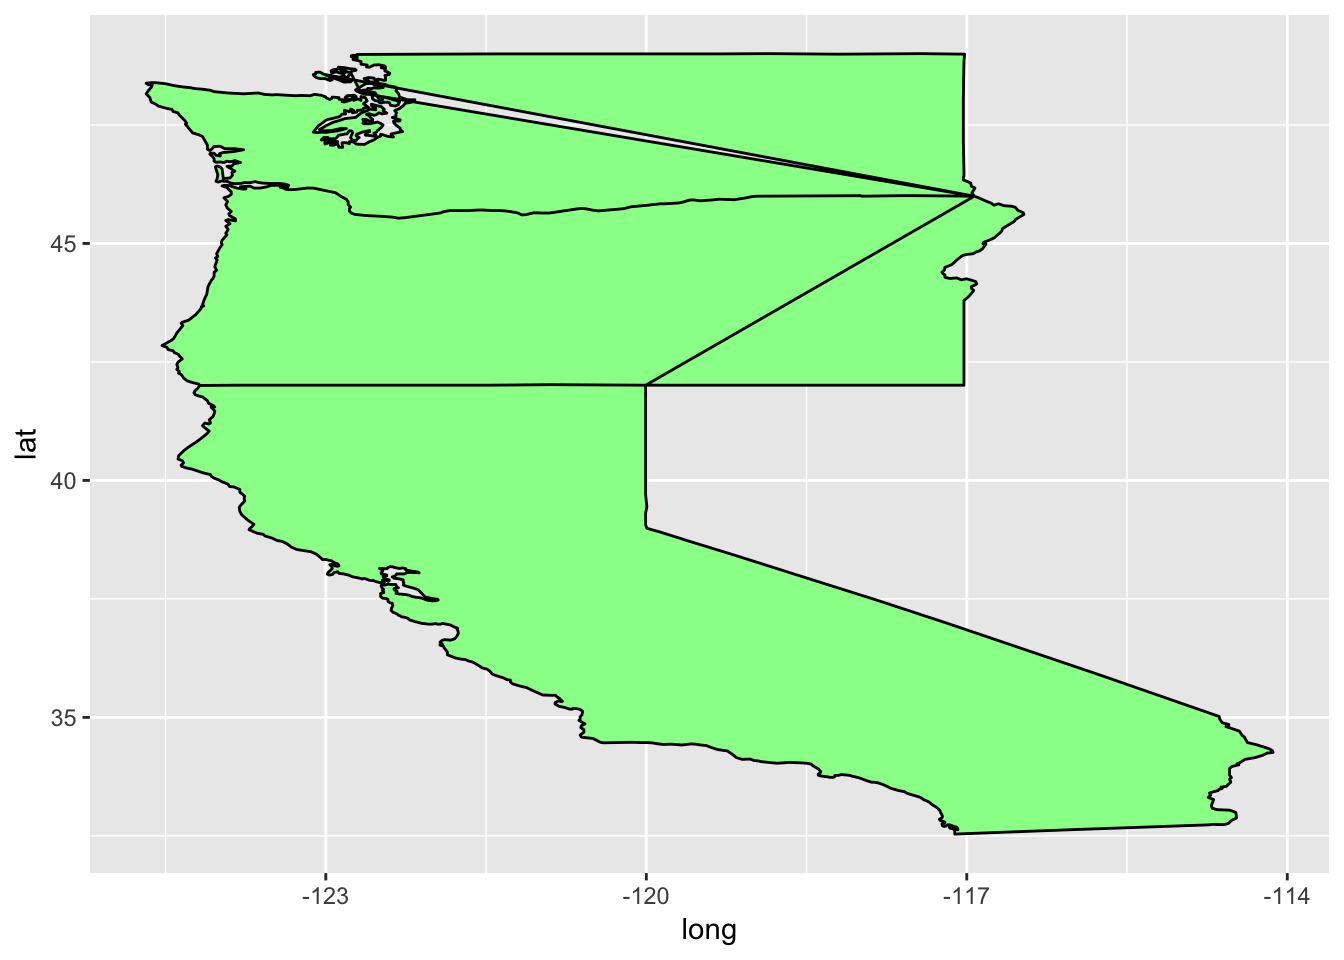
\includegraphics{bookdown-demo_files/figure-latex/unnamed-chunk-69-1.pdf}
\end{itemize}

\subsubsection{Man that is ugly!!}\label{man-that-is-ugly}

\begin{itemize}
\item
  I am just keeping people on their toes. What have we forgotten here?

  \begin{itemize}
  \tightlist
  \item
    \texttt{group}
  \item
    \texttt{coord\_quickmap()}
  \end{itemize}
\item
  Let's put those back in there:

\begin{Shaded}
\begin{Highlighting}[]
\KeywordTok{ggplot}\NormalTok{(}\DataTypeTok{data =} \NormalTok{west_coast) +}\StringTok{ }
\StringTok{  }\KeywordTok{geom_polygon}\NormalTok{(}\KeywordTok{aes}\NormalTok{(}\DataTypeTok{x =} \NormalTok{long, }\DataTypeTok{y =} \NormalTok{lat, }\DataTypeTok{group =} \NormalTok{group), }\DataTypeTok{fill =} \StringTok{"palegreen"}\NormalTok{, }\DataTypeTok{color =} \StringTok{"black"}\NormalTok{) +}\StringTok{ }
\StringTok{  }\KeywordTok{coord_quickmap}\NormalTok{()}
\end{Highlighting}
\end{Shaded}

  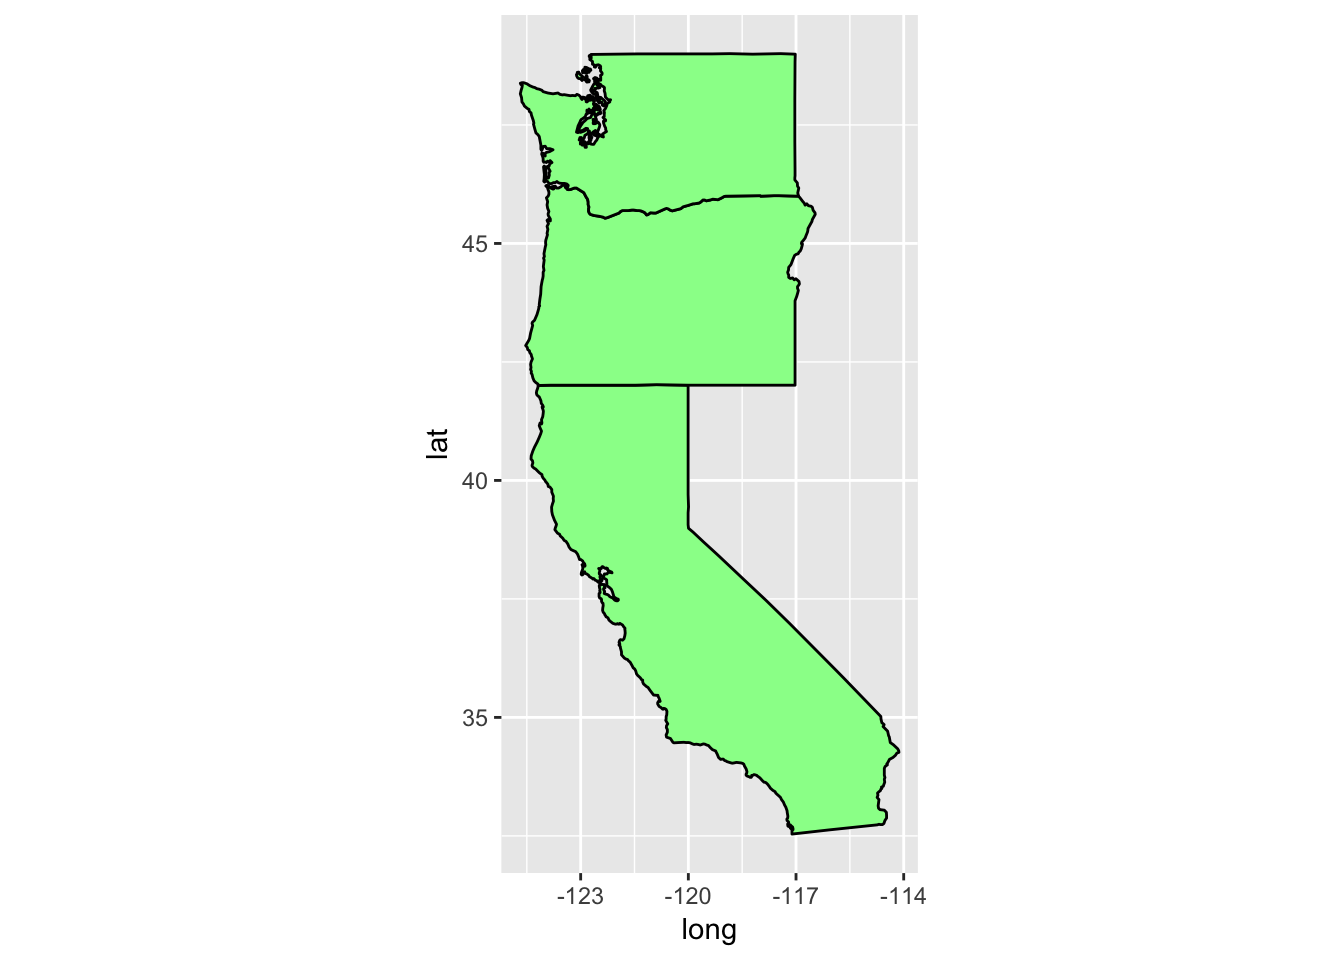
\includegraphics{bookdown-demo_files/figure-latex/unnamed-chunk-70-1.pdf}
\end{itemize}

Phew! That is a little better!

\subsubsection{Zoom in on California and look at
counties}\label{zoom-in-on-california-and-look-at-counties}

\begin{itemize}
\item
  Getting the california data is easy:

\begin{Shaded}
\begin{Highlighting}[]
\NormalTok{ca_df <-}\StringTok{ }\KeywordTok{subset}\NormalTok{(states, region ==}\StringTok{ "california"}\NormalTok{)}

\KeywordTok{head}\NormalTok{(ca_df)}
\end{Highlighting}
\end{Shaded}

\begin{verbatim}
##          long      lat group order     region subregion
## 667 -120.0060 42.00927     4   667 california      <NA>
## 668 -120.0060 41.20139     4   668 california      <NA>
## 669 -120.0060 39.70024     4   669 california      <NA>
## 670 -119.9946 39.44241     4   670 california      <NA>
## 671 -120.0060 39.31636     4   671 california      <NA>
## 672 -120.0060 39.16166     4   672 california      <NA>
\end{verbatim}
\item
  Now, let's also get the county lines there

\begin{Shaded}
\begin{Highlighting}[]
\NormalTok{counties <-}\StringTok{ }\KeywordTok{map_data}\NormalTok{(}\StringTok{"county"}\NormalTok{)}
\NormalTok{ca_county <-}\StringTok{ }\KeywordTok{subset}\NormalTok{(counties, region ==}\StringTok{ "california"}\NormalTok{)}

\KeywordTok{head}\NormalTok{(ca_county)}
\end{Highlighting}
\end{Shaded}

\begin{verbatim}
##           long      lat group order     region subregion
## 6965 -121.4785 37.48290   157  6965 california   alameda
## 6966 -121.5129 37.48290   157  6966 california   alameda
## 6967 -121.8853 37.48290   157  6967 california   alameda
## 6968 -121.8968 37.46571   157  6968 california   alameda
## 6969 -121.9254 37.45998   157  6969 california   alameda
## 6970 -121.9483 37.47717   157  6970 california   alameda
\end{verbatim}
\item
  Plot the state first but let's ditch the axes gridlines, and gray
  background by using the super-wonderful \texttt{theme\_void()} which
  leaves off everything except the geoms.

\begin{Shaded}
\begin{Highlighting}[]
\NormalTok{ca_base <-}\StringTok{ }\KeywordTok{ggplot}\NormalTok{(}\DataTypeTok{data =} \NormalTok{ca_df, }\DataTypeTok{mapping =} \KeywordTok{aes}\NormalTok{(}\DataTypeTok{x =} \NormalTok{long, }\DataTypeTok{y =} \NormalTok{lat, }\DataTypeTok{group =} \NormalTok{group)) +}\StringTok{ }
\StringTok{  }\KeywordTok{coord_quickmap}\NormalTok{() +}\StringTok{ }
\StringTok{  }\KeywordTok{geom_polygon}\NormalTok{(}\DataTypeTok{color =} \StringTok{"black"}\NormalTok{, }\DataTypeTok{fill =} \StringTok{"gray"}\NormalTok{)}
\NormalTok{ca_base +}\StringTok{ }\KeywordTok{theme_void}\NormalTok{()}
\end{Highlighting}
\end{Shaded}

  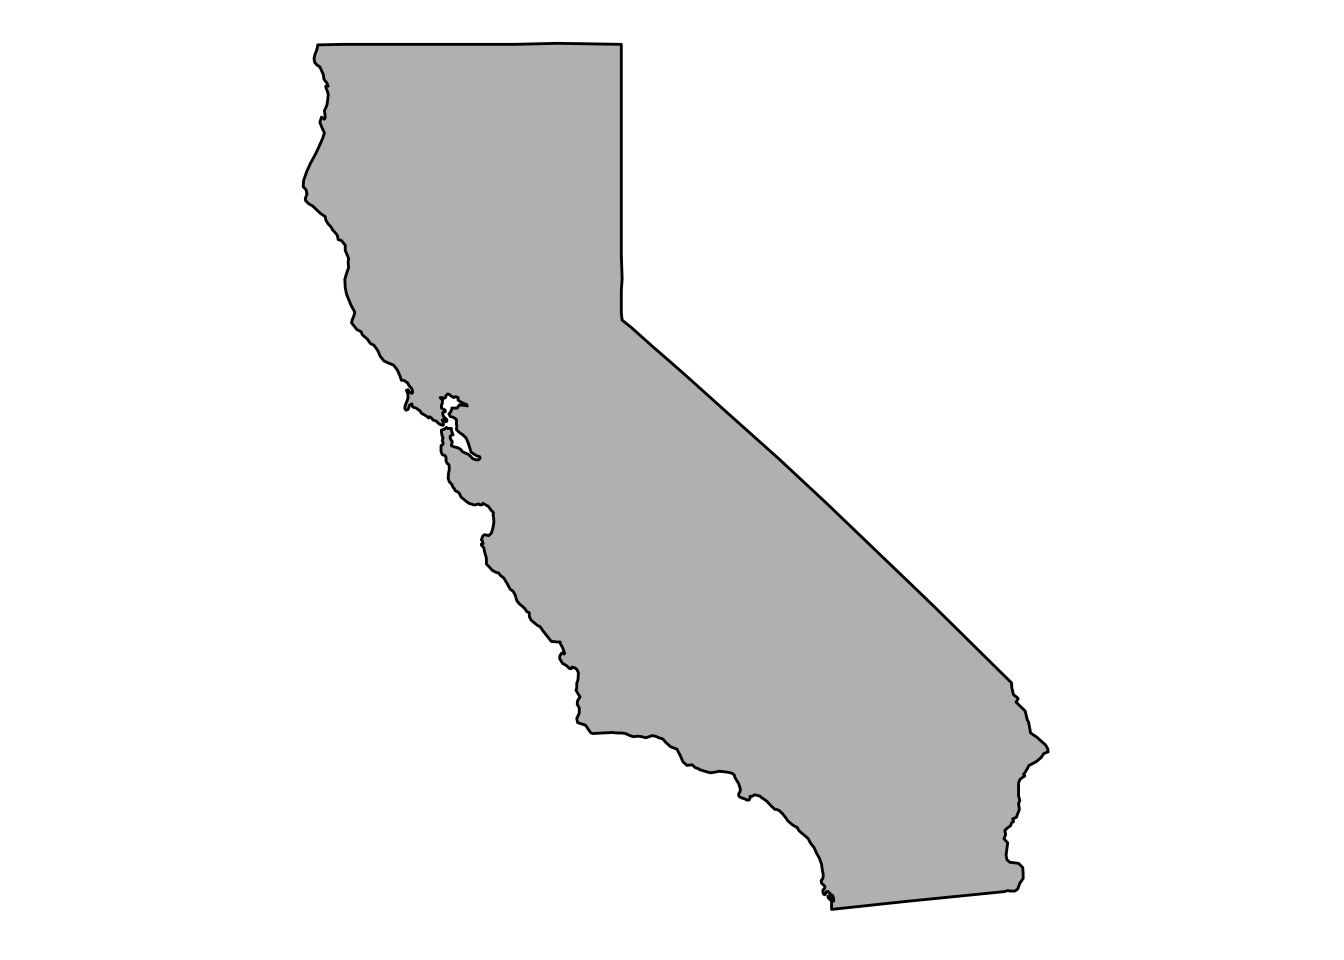
\includegraphics{bookdown-demo_files/figure-latex/unnamed-chunk-73-1.pdf}
\item
  Now plot the county boundaries in white:

\begin{Shaded}
\begin{Highlighting}[]
\NormalTok{ca_base +}\StringTok{ }\KeywordTok{theme_void}\NormalTok{() +}\StringTok{ }
\StringTok{  }\KeywordTok{geom_polygon}\NormalTok{(}\DataTypeTok{data =} \NormalTok{ca_county, }\DataTypeTok{fill =} \OtherTok{NA}\NormalTok{, }\DataTypeTok{color =} \StringTok{"white"}\NormalTok{) +}
\StringTok{  }\KeywordTok{geom_polygon}\NormalTok{(}\DataTypeTok{color =} \StringTok{"black"}\NormalTok{, }\DataTypeTok{fill =} \OtherTok{NA}\NormalTok{)  }\CommentTok{# get the state border back on top}
\end{Highlighting}
\end{Shaded}

  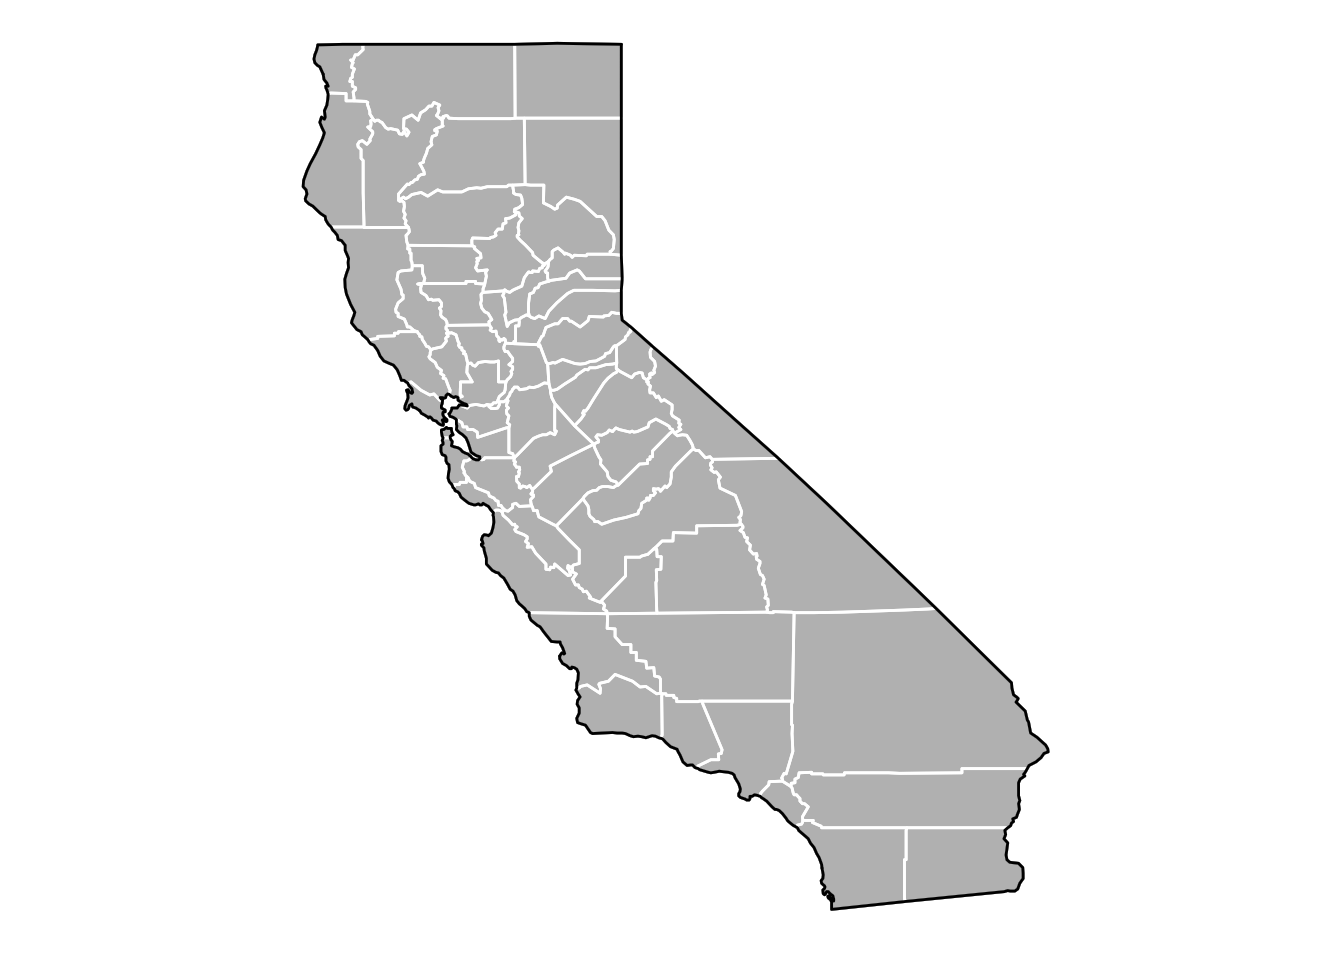
\includegraphics{bookdown-demo_files/figure-latex/unnamed-chunk-74-1.pdf}
\end{itemize}

\subsubsection{Get some facts about the
counties}\label{get-some-facts-about-the-counties}

\begin{itemize}
\tightlist
\item
  The above is pretty cool, but it seems like it would be a lot cooler
  if we could plot some information about those counties.\\
\item
  Now I can go to wikipedia or
  \url{http://www.california-demographics.com/counties_by_population}
  and grab population and area data for each county.
\item
  In fact, I copied their little table on Wikipedia and saved it into
  \texttt{inputs/ca-counties-wikipedia.txt}. In full disclosure I also
  edited the name of San Francisco from ``City and County of San
  Francisco'' to ``San Francisco County'' to be like the others (and not
  break my regex!)
\item
  2016 Edit! I had originally pumped the matrix resulting from the
  \texttt{str\_match} below through a few other \texttt{stringr}
  function (like \texttt{str\_replace\_all}) which, apparently, in an
  older version of \texttt{stringr} maintained the matrix form, but in a
  newer version, squashed everything into a vector. This was kindly
  noted by hueykwik
  \href{https://github.com/eriqande/rep-res-course/issues/74}{in this
  issue}. So the code below is modified from what it used to be, but
  seems to work now. Just as an aside, in the years since I put this
  course together, things have changed quite a bit in the data analysis
  world, and, if I re-did the course today I would spend almost all my
  time in the \href{http://r4ds.had.co.nz/}{tidyverse}.
\item
  Watch this regex fun:
\end{itemize}

\begin{Shaded}
\begin{Highlighting}[]
    \KeywordTok{library}\NormalTok{(stringr)}
    \KeywordTok{library}\NormalTok{(dplyr)}

    \CommentTok{# make a data frame}
    \NormalTok{x <-}\StringTok{ }\KeywordTok{readLines}\NormalTok{(}\StringTok{"inputs/ca-counties-wikipedia.txt"}\NormalTok{)}
    \NormalTok{pop_and_area <-}\StringTok{ }\KeywordTok{str_match}\NormalTok{(x, }\StringTok{"^([a-zA-Z ]+)County}\CharTok{\textbackslash{}t}\StringTok{.*}\CharTok{\textbackslash{}t}\StringTok{([0-9,]\{2,10\})}\CharTok{\textbackslash{}t}\StringTok{([0-9,]\{2,10\}) sq mi$"}\NormalTok{)[, -}\DecValTok{1}\NormalTok{] %>%}
\StringTok{      }\KeywordTok{na.omit}\NormalTok{() %>%}
\StringTok{      }\KeywordTok{as.data.frame}\NormalTok{(}\DataTypeTok{stringsAsFactors =} \OtherTok{FALSE}\NormalTok{) %>%}
\StringTok{      }\KeywordTok{mutate}\NormalTok{(}\DataTypeTok{subregion =} \KeywordTok{str_trim}\NormalTok{(V1) %>%}\StringTok{ }\KeywordTok{tolower}\NormalTok{(),}
             \DataTypeTok{population =} \KeywordTok{as.numeric}\NormalTok{(}\KeywordTok{str_replace_all}\NormalTok{(V2, }\StringTok{","}\NormalTok{, }\StringTok{""}\NormalTok{)),}
             \DataTypeTok{area =} \KeywordTok{as.numeric}\NormalTok{(}\KeywordTok{str_replace_all}\NormalTok{(V3, }\StringTok{","}\NormalTok{, }\StringTok{""}\NormalTok{))}
      \NormalTok{) %>%}
\StringTok{      }\KeywordTok{select}\NormalTok{(subregion, population, area) %>%}
\StringTok{      }\KeywordTok{tbl_df}\NormalTok{()}
    
    \KeywordTok{head}\NormalTok{(pop_and_area)}
\end{Highlighting}
\end{Shaded}

\begin{verbatim}
## # A tibble: 6 × 3
##   subregion population  area
##       <chr>      <dbl> <dbl>
## 1   alameda    1578891   738
## 2    alpine       1159   739
## 3    amador      36519   593
## 4     butte     222090  1640
## 5 calaveras      44515  1020
## 6    colusa      21358  1151
\end{verbatim}

\begin{itemize}
\item
  We now have the numbers that we want, but we need to attach those to
  every point on polygons of the counties. This is a job for
  \texttt{inner\_join} from the \texttt{dplyr} package

\begin{Shaded}
\begin{Highlighting}[]
\NormalTok{cacopa <-}\StringTok{ }\KeywordTok{inner_join}\NormalTok{(ca_county, pop_and_area, }\DataTypeTok{by =} \StringTok{"subregion"}\NormalTok{)}
\end{Highlighting}
\end{Shaded}
\item
  And finally, add a column of \texttt{people\_per\_mile}:

\begin{Shaded}
\begin{Highlighting}[]
\NormalTok{cacopa$people_per_mile <-}\StringTok{ }\NormalTok{cacopa$population /}\StringTok{ }\NormalTok{cacopa$area}

\KeywordTok{head}\NormalTok{(cacopa)}
\end{Highlighting}
\end{Shaded}

\begin{verbatim}
##        long      lat group order     region subregion population area
## 1 -121.4785 37.48290   157  6965 california   alameda    1578891  738
## 2 -121.5129 37.48290   157  6966 california   alameda    1578891  738
## 3 -121.8853 37.48290   157  6967 california   alameda    1578891  738
## 4 -121.8968 37.46571   157  6968 california   alameda    1578891  738
## 5 -121.9254 37.45998   157  6969 california   alameda    1578891  738
## 6 -121.9483 37.47717   157  6970 california   alameda    1578891  738
##   people_per_mile
## 1        2139.419
## 2        2139.419
## 3        2139.419
## 4        2139.419
## 5        2139.419
## 6        2139.419
\end{verbatim}
\end{itemize}

\subsubsection{Now plot population density by
county}\label{now-plot-population-density-by-county}

If you were needing a little more elbow room in the great Golden State,
this shows you where you can find it:

\begin{Shaded}
\begin{Highlighting}[]
\CommentTok{# prepare to drop the axes and ticks but leave the guides and legends}
\CommentTok{# We can't just throw down a theme_void()!}
\NormalTok{ditch_the_axes <-}\StringTok{ }\KeywordTok{theme}\NormalTok{(}
  \DataTypeTok{axis.text =} \KeywordTok{element_blank}\NormalTok{(),}
  \DataTypeTok{axis.line =} \KeywordTok{element_blank}\NormalTok{(),}
  \DataTypeTok{axis.ticks =} \KeywordTok{element_blank}\NormalTok{(),}
  \DataTypeTok{panel.border =} \KeywordTok{element_blank}\NormalTok{(),}
  \DataTypeTok{panel.grid =} \KeywordTok{element_blank}\NormalTok{(),}
  \DataTypeTok{axis.title =} \KeywordTok{element_blank}\NormalTok{()}
  \NormalTok{)}

\NormalTok{elbow_room1 <-}\StringTok{ }\NormalTok{ca_base +}\StringTok{ }
\StringTok{      }\KeywordTok{geom_polygon}\NormalTok{(}\DataTypeTok{data =} \NormalTok{cacopa, }\KeywordTok{aes}\NormalTok{(}\DataTypeTok{fill =} \NormalTok{people_per_mile), }\DataTypeTok{color =} \StringTok{"white"}\NormalTok{) +}
\StringTok{      }\KeywordTok{geom_polygon}\NormalTok{(}\DataTypeTok{color =} \StringTok{"black"}\NormalTok{, }\DataTypeTok{fill =} \OtherTok{NA}\NormalTok{) +}
\StringTok{      }\KeywordTok{theme_bw}\NormalTok{() +}
\StringTok{      }\NormalTok{ditch_the_axes}

\NormalTok{elbow_room1 }
\end{Highlighting}
\end{Shaded}

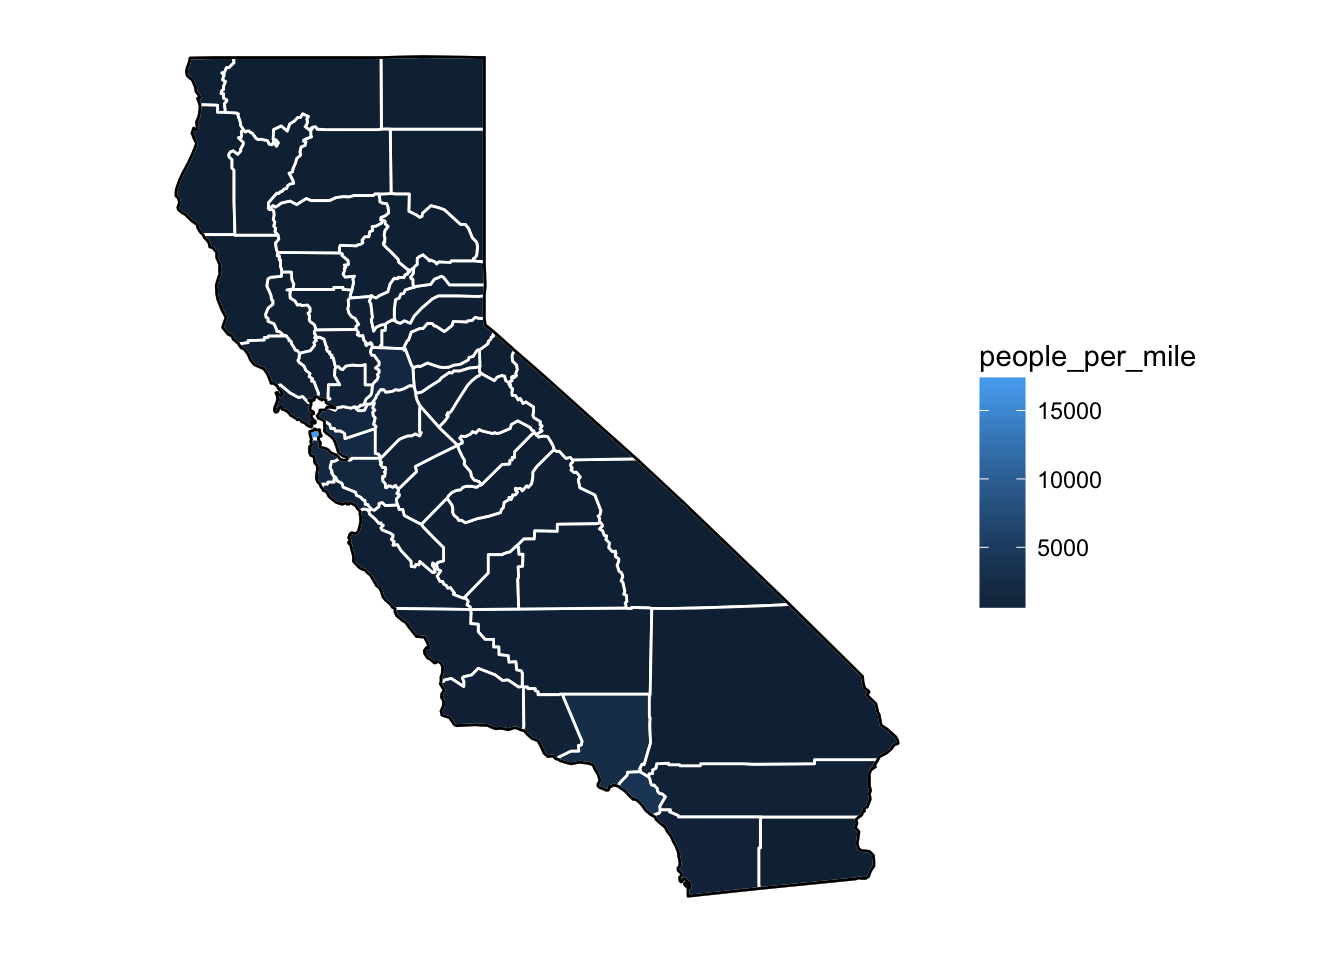
\includegraphics{bookdown-demo_files/figure-latex/unnamed-chunk-78-1.pdf}

\subsubsection{Lame!}\label{lame}

\begin{itemize}
\tightlist
\item
  The popuation density in San Francisco is so great that it makes it
  hard to discern differences between other areas.
\item
  This is a job for a scale transformation. Let's take the log-base-10
  of the population density.
\item
  Instead of making a new column which is log10 of the
  \texttt{people\_per\_mile} we can just apply the transformation in the
  gradient using the \texttt{trans} argument
\end{itemize}

\begin{Shaded}
\begin{Highlighting}[]
\NormalTok{elbow_room1 +}\StringTok{ }\KeywordTok{scale_fill_gradient}\NormalTok{(}\DataTypeTok{trans =} \StringTok{"log10"}\NormalTok{)}
\end{Highlighting}
\end{Shaded}

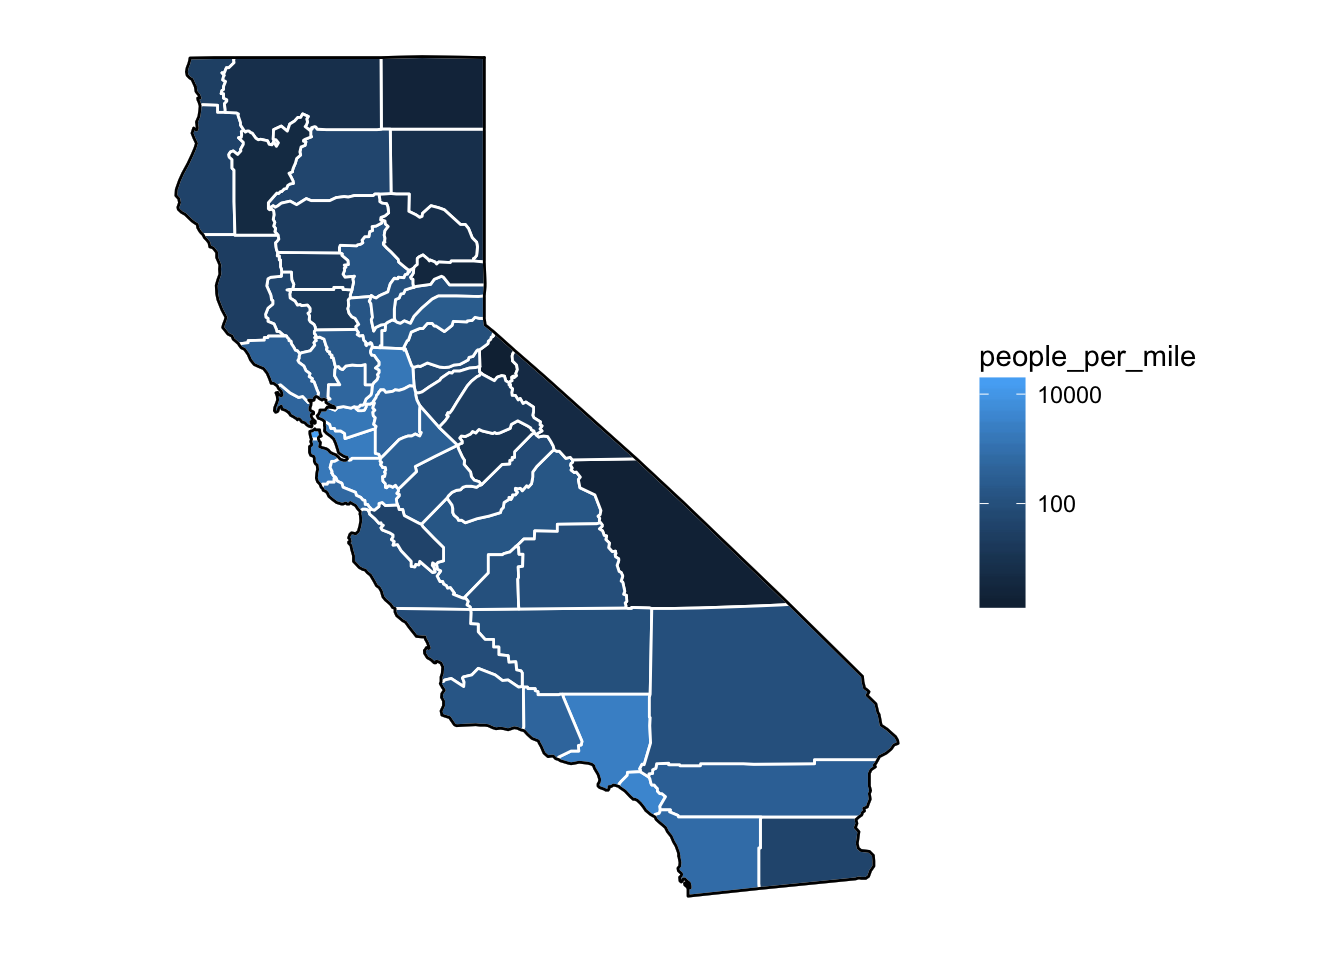
\includegraphics{bookdown-demo_files/figure-latex/unnamed-chunk-79-1.pdf}

\subsubsection{Still not great}\label{still-not-great}

I personally like more color than ggplot uses in its default gradient.
In that respect I gravitate more toward Matlab's default color gradient.
Can we do something similar with \texttt{ggplot}?

\begin{Shaded}
\begin{Highlighting}[]
\NormalTok{eb2 <-}\StringTok{ }\NormalTok{elbow_room1 +}\StringTok{ }
\StringTok{    }\KeywordTok{scale_fill_gradientn}\NormalTok{(}\DataTypeTok{colours =} \KeywordTok{rev}\NormalTok{(}\KeywordTok{rainbow}\NormalTok{(}\DecValTok{7}\NormalTok{)),}
                         \DataTypeTok{breaks =} \KeywordTok{c}\NormalTok{(}\DecValTok{2}\NormalTok{, }\DecValTok{4}\NormalTok{, }\DecValTok{10}\NormalTok{, }\DecValTok{100}\NormalTok{, }\DecValTok{1000}\NormalTok{, }\DecValTok{10000}\NormalTok{),}
                         \DataTypeTok{trans =} \StringTok{"log10"}\NormalTok{)}
\NormalTok{eb2}
\end{Highlighting}
\end{Shaded}

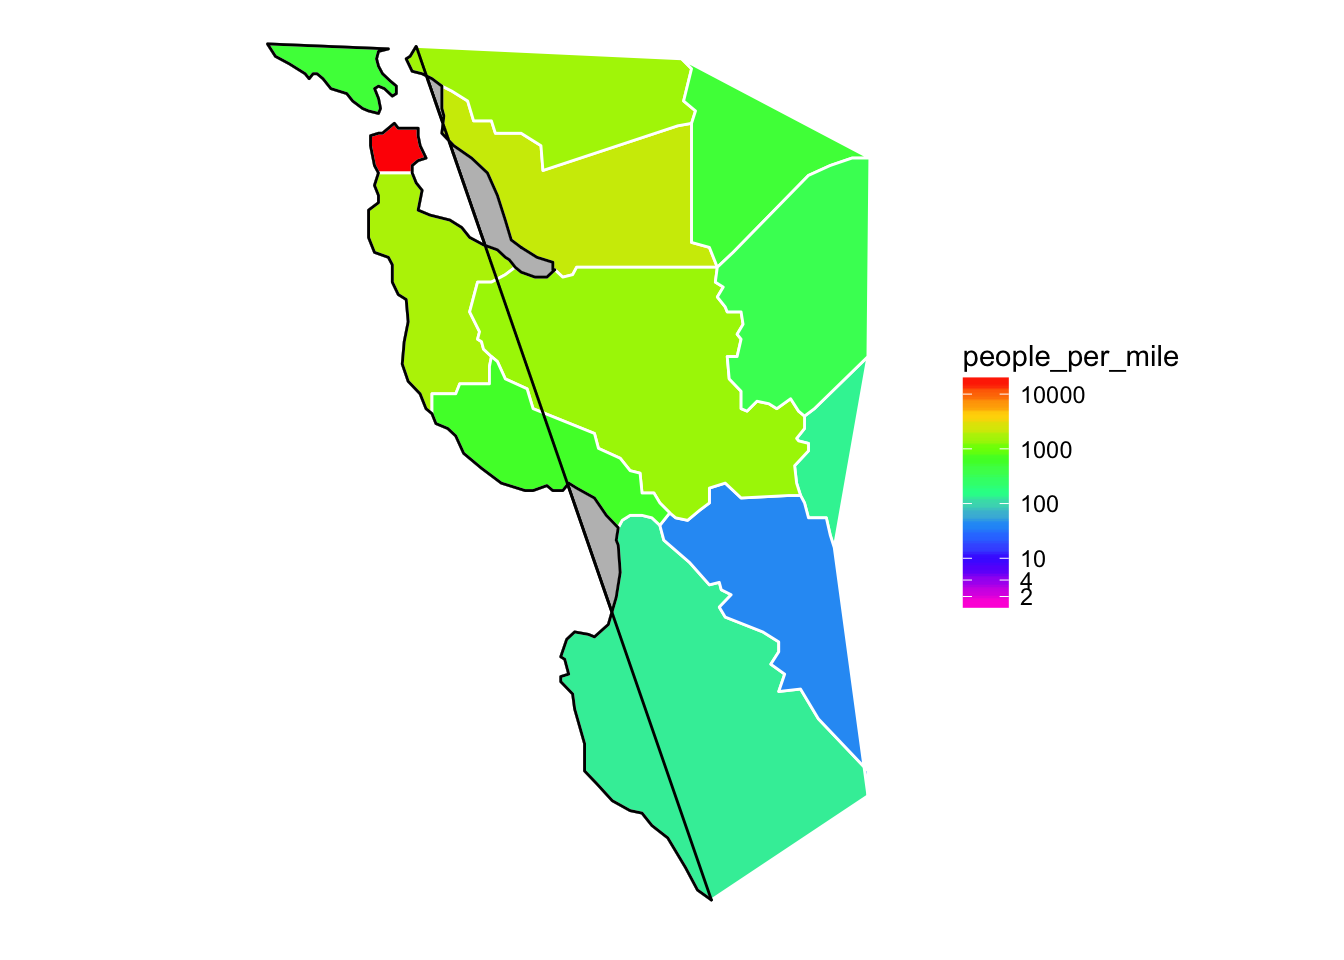
\includegraphics{bookdown-demo_files/figure-latex/unnamed-chunk-80-1.pdf}

That is reasonably cool.

\subsection{zoom in?}\label{zoom-in}

Note that the scale of these maps from package \texttt{maps} are not
great. We can zoom in to the Bay region, and it sort of works
scale-wise, but if we wanted to zoom in more, it would be tough.

Let's try!

\begin{Shaded}
\begin{Highlighting}[]
\NormalTok{eb2 +}\StringTok{ }\KeywordTok{xlim}\NormalTok{(-}\DecValTok{123}\NormalTok{, -}\FloatTok{121.0}\NormalTok{) +}\StringTok{ }\KeywordTok{ylim}\NormalTok{(}\DecValTok{36}\NormalTok{, }\DecValTok{38}\NormalTok{)}
\end{Highlighting}
\end{Shaded}

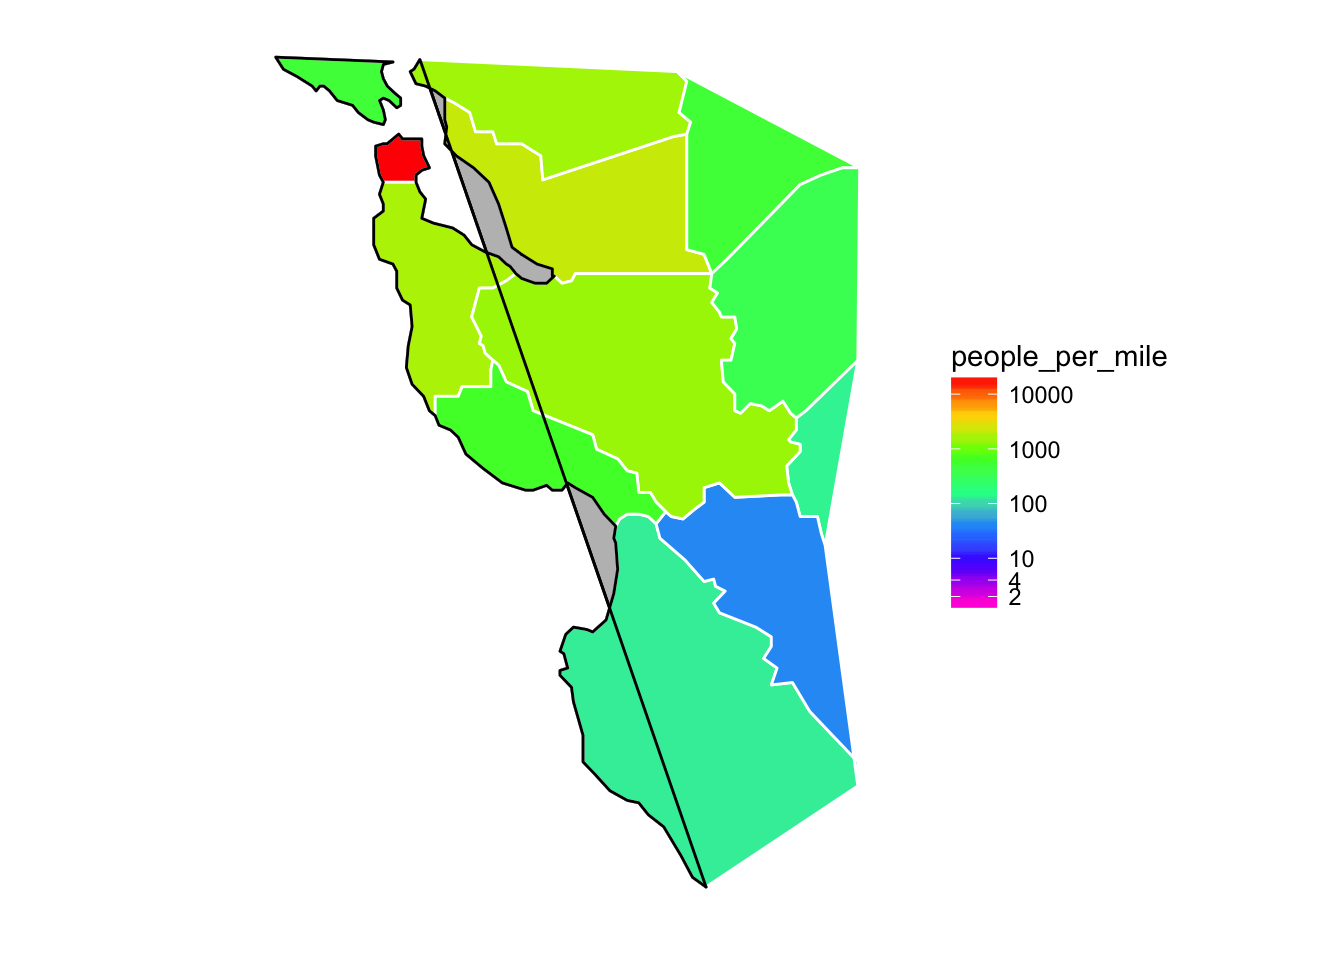
\includegraphics{bookdown-demo_files/figure-latex/unnamed-chunk-81-1.pdf}

\begin{itemize}
\tightlist
\item
  Whoa! That is an epic fail. Why?
\item
  Recall that \texttt{geom\_polygon()} connects the end point of a
  \texttt{group} to its starting point.
\item
  And the kicker: the \texttt{xlim} and \texttt{ylim} functions in
  \texttt{ggplot2} discard all the data that is not within the plot
  area.

  \begin{itemize}
  \tightlist
  \item
    Hence there are new starting points and ending points for some
    groups (or in this case the black-line permiter of California) and
    those points get connected. Not good.
  \end{itemize}
\end{itemize}

\subsection{True zoom.}\label{true-zoom.}

\begin{itemize}
\item
  If you want to keep all the data the same but just zoom in, you can
  use the \texttt{xlim} and \texttt{ylim} arguments to
  \texttt{coord\_cartesian()}. Though, to keep the aspect ratio correct
  we must use \texttt{coord\_quickmap()} instead of
  \texttt{coord\_cartesian()}.
\item
  This chops stuff off but doesn't discard it from the data set:

\begin{Shaded}
\begin{Highlighting}[]
\NormalTok{eb2 +}\StringTok{ }\KeywordTok{coord_quickmap}\NormalTok{(}\DataTypeTok{xlim =} \KeywordTok{c}\NormalTok{(-}\DecValTok{123}\NormalTok{, -}\FloatTok{121.0}\NormalTok{),  }\DataTypeTok{ylim =} \KeywordTok{c}\NormalTok{(}\DecValTok{36}\NormalTok{, }\DecValTok{38}\NormalTok{))}
\end{Highlighting}
\end{Shaded}

  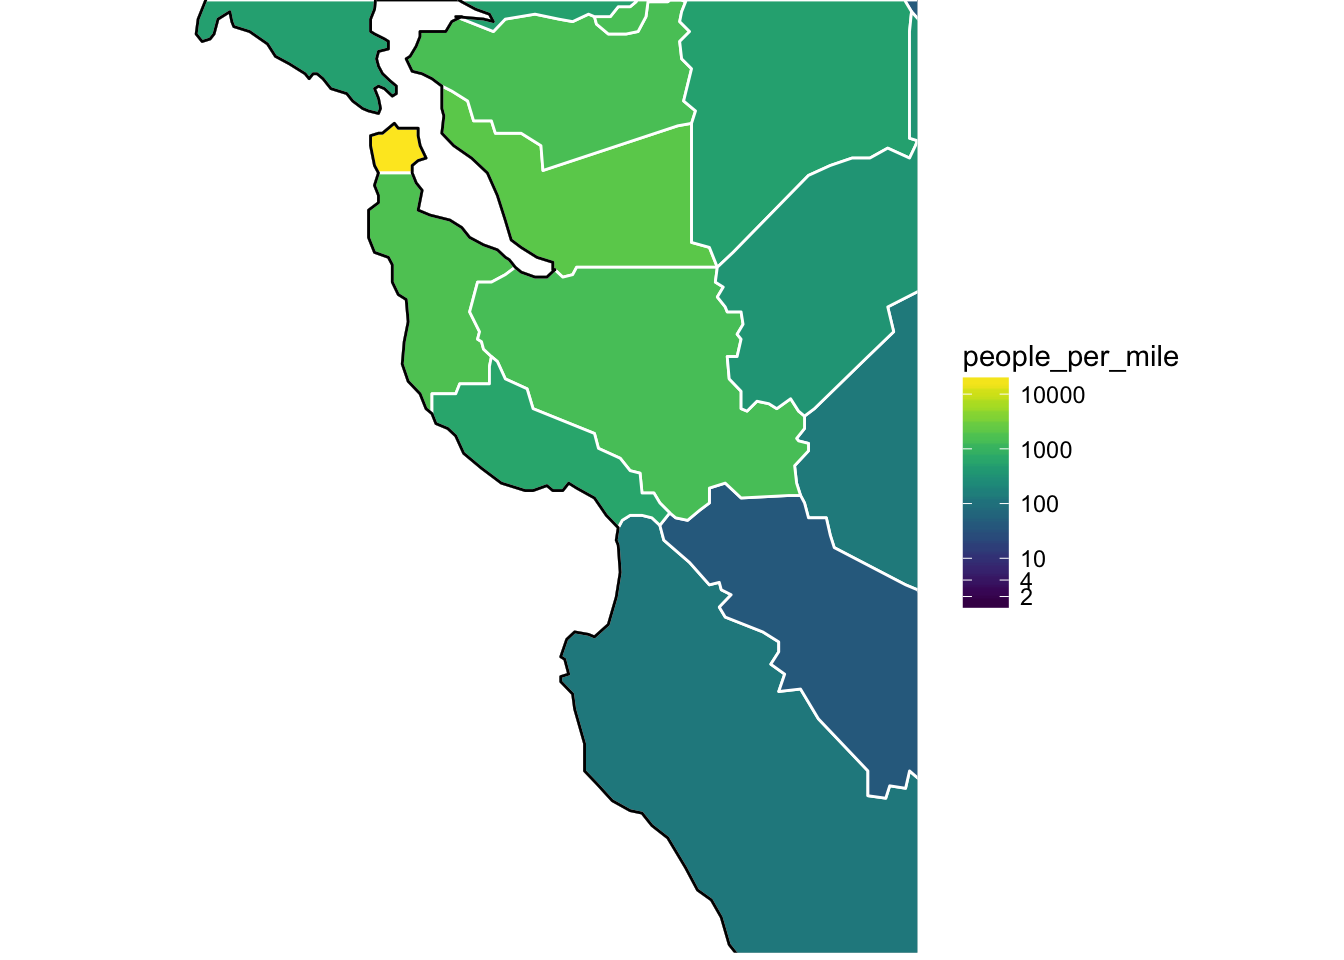
\includegraphics{bookdown-demo_files/figure-latex/unnamed-chunk-82-1.pdf}
\end{itemize}

Side Note: The coastline in the \texttt{maps} package is pretty
low-resolution, and looks like a heap of bird droppings when you zoom
way in on it.

If you want to get much more accurate coastlines, you can use better
data sources like NOAA's
\href{https://www.ngdc.noaa.gov/mgg/shorelines/gshhs.html}{GSHHS}: A
Global Self-consistent, Hierarchical, High-resolution Geography
Database. I have a blog post about that at
\url{http://eriqande.github.io/2014/12/17/compare-map-resolutions.html}.

\section{ggmap}\label{ggmap-hooray}

The \texttt{ggmap} package is a nice way to make quick maps with decent
backgrounds! We will talk later about how to get better-looking maps at
some resolutions by using shapefiles and rasters from
naturalearthdata.com but \texttt{ggmap} will get you 95\% of the way
there with a lot less of the work!

If you don't have it, get the most updated version off GitHub:

\begin{Shaded}
\begin{Highlighting}[]
\NormalTok{devtools::}\KeywordTok{install_github}\NormalTok{(}\StringTok{"dkahle/ggmap"}\NormalTok{)}
\end{Highlighting}
\end{Shaded}

And load it like so:

\begin{Shaded}
\begin{Highlighting}[]
\KeywordTok{library}\NormalTok{(ggmap)}
\end{Highlighting}
\end{Shaded}

\subsection{Three examples}\label{three-examples}

\begin{itemize}
\tightlist
\item
  I am going to run through three examples. Working from the small
  spatial scale up to a larger spatial scale.

  \begin{enumerate}
  \def\labelenumi{\arabic{enumi}.}
  \tightlist
  \item
    Named ``sampling'' points on the Sisquoc River from the
    ``Sisquoctober Adventure''
  \item
    A GPS track from a short bike ride in Wilder Ranch.
  \item
    Fish sampling locations from the coded wire tag data base.
  \end{enumerate}
\end{itemize}

\subsection{How ggmap works}\label{how-ggmap-works}

\begin{itemize}
\tightlist
\item
  ggmap simplifies the process of downloading base maps from Google or
  Open Street Maps or Stamen Maps to use in the background of your
  plots.
\item
  It also sets the axis scales, etc, in a nice way.\\
\item
  Once you have gotten your maps, you make a call with \texttt{ggmap()}
  much as you would with \texttt{ggplot()}
\item
  Let's do by example.
\end{itemize}

\subsection{Sisquoctober}\label{sisquoctober}

\begin{itemize}
\item
  Here is a small data frame of points from the Sisquoc River.

\begin{Shaded}
\begin{Highlighting}[]
\NormalTok{sisquoc <-}\StringTok{ }\KeywordTok{read.table}\NormalTok{(}\StringTok{"inputs/sisquoc-points.txt"}\NormalTok{, }\DataTypeTok{sep =} \StringTok{"}\CharTok{\textbackslash{}t}\StringTok{"}\NormalTok{, }\DataTypeTok{header =} \OtherTok{TRUE}\NormalTok{)}
\NormalTok{sisquoc}
\end{Highlighting}
\end{Shaded}

\begin{verbatim}
##     name       lon      lat
## 1    a17 -119.7603 34.75474
## 2 a20-24 -119.7563 34.75380
## 3 a25-28 -119.7537 34.75371
## 4 a18,19 -119.7573 34.75409
## 5 a35,36 -119.7467 34.75144
## 6    a31 -119.7478 34.75234
## 7    a38 -119.7447 34.75230
## 8    a43 -119.7437 34.75251
\end{verbatim}

\begin{Shaded}
\begin{Highlighting}[]
\CommentTok{# note that ggmap tends to use "lon" instead of "long" for longitude.}
\end{Highlighting}
\end{Shaded}
\end{itemize}

Grab google map tiles by specifying a center and a zoom. They are always
squarish tiles\ldots{}

\begin{Shaded}
\begin{Highlighting}[]
\KeywordTok{get_googlemap}\NormalTok{(}\DataTypeTok{center =} \KeywordTok{c}\NormalTok{(}\KeywordTok{mean}\NormalTok{(sisquoc$lon), }\KeywordTok{mean}\NormalTok{(sisquoc$lat)), }\DataTypeTok{zoom =} \DecValTok{15}\NormalTok{) %>%}
\StringTok{  }\KeywordTok{ggmap}\NormalTok{() +}
\StringTok{  }\KeywordTok{geom_point}\NormalTok{(}\DataTypeTok{data =} \NormalTok{sisquoc, }\DataTypeTok{mapping =} \KeywordTok{aes}\NormalTok{(}\DataTypeTok{x =} \NormalTok{lon, }\DataTypeTok{y =} \NormalTok{lat), }\DataTypeTok{color =} \StringTok{"red"}\NormalTok{)}
\end{Highlighting}
\end{Shaded}

\begin{verbatim}
## Source : https://maps.googleapis.com/maps/api/staticmap?center=34.753117,-119.751324&zoom=15&size=640x640&scale=2&maptype=terrain
\end{verbatim}

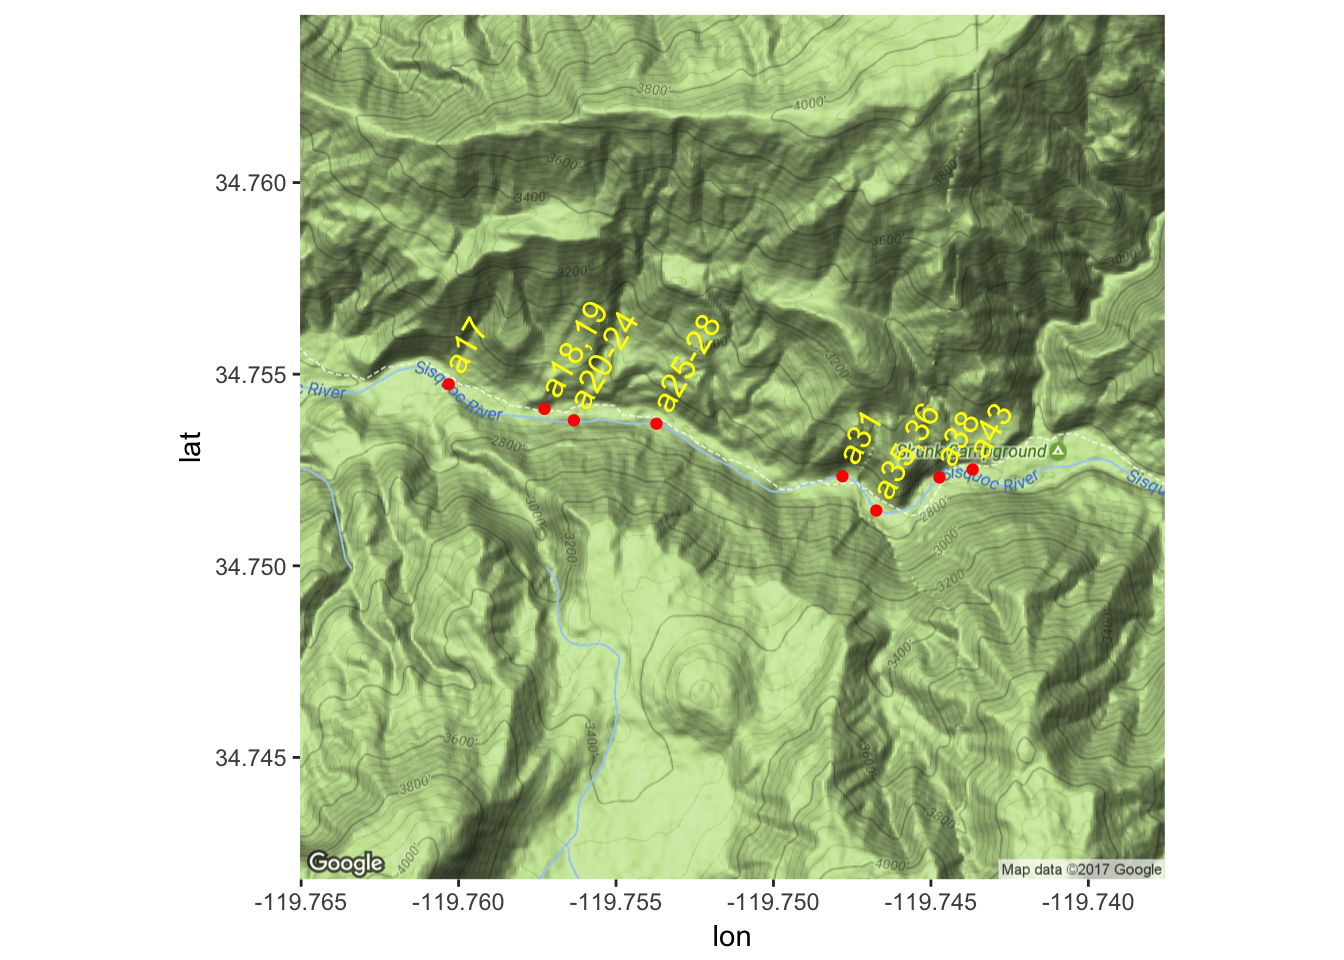
\includegraphics{bookdown-demo_files/figure-latex/unnamed-chunk-86-1.pdf}

Here with satellite photos:

\begin{Shaded}
\begin{Highlighting}[]
\KeywordTok{get_googlemap}\NormalTok{(}\DataTypeTok{center =} \KeywordTok{c}\NormalTok{(}\KeywordTok{mean}\NormalTok{(sisquoc$lon), }\KeywordTok{mean}\NormalTok{(sisquoc$lat)), }
              \DataTypeTok{zoom =} \DecValTok{15}\NormalTok{,}
              \DataTypeTok{maptype =} \StringTok{"satellite"}\NormalTok{) %>%}
\StringTok{  }\KeywordTok{ggmap}\NormalTok{() +}
\StringTok{  }\KeywordTok{geom_point}\NormalTok{(}\DataTypeTok{data =} \NormalTok{sisquoc, }\DataTypeTok{mapping =} \KeywordTok{aes}\NormalTok{(}\DataTypeTok{x =} \NormalTok{lon, }\DataTypeTok{y =} \NormalTok{lat), }\DataTypeTok{color =} \StringTok{"red"}\NormalTok{)}
\end{Highlighting}
\end{Shaded}

\begin{verbatim}
## Source : https://maps.googleapis.com/maps/api/staticmap?center=34.753117,-119.751324&zoom=15&size=640x640&scale=2&maptype=satellite
\end{verbatim}

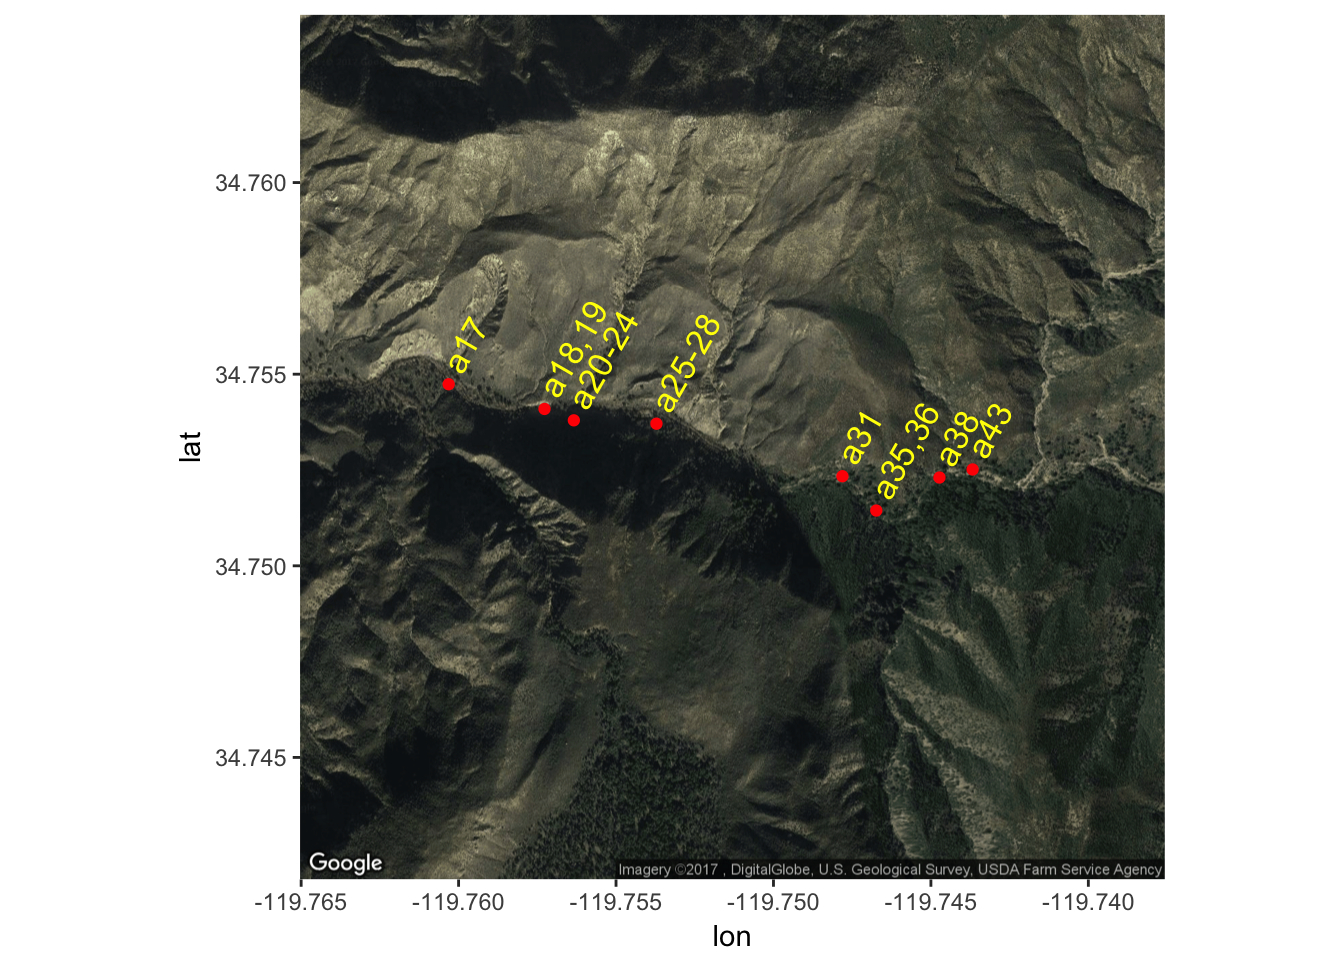
\includegraphics{bookdown-demo_files/figure-latex/unnamed-chunk-87-1.pdf}

Out of curiosity, let's see what Big Creek looks like:

\begin{Shaded}
\begin{Highlighting}[]
\KeywordTok{get_googlemap}\NormalTok{(}\DataTypeTok{center =} \KeywordTok{c}\NormalTok{(-}\FloatTok{121.599271}\NormalTok{, }\FloatTok{36.071003}\NormalTok{), }\DataTypeTok{zoom =} \DecValTok{15}\NormalTok{) %>%}
\StringTok{  }\KeywordTok{ggmap}\NormalTok{() }
\end{Highlighting}
\end{Shaded}

\begin{verbatim}
## Source : https://maps.googleapis.com/maps/api/staticmap?center=36.071003,-121.599271&zoom=15&size=640x640&scale=2&maptype=terrain
\end{verbatim}

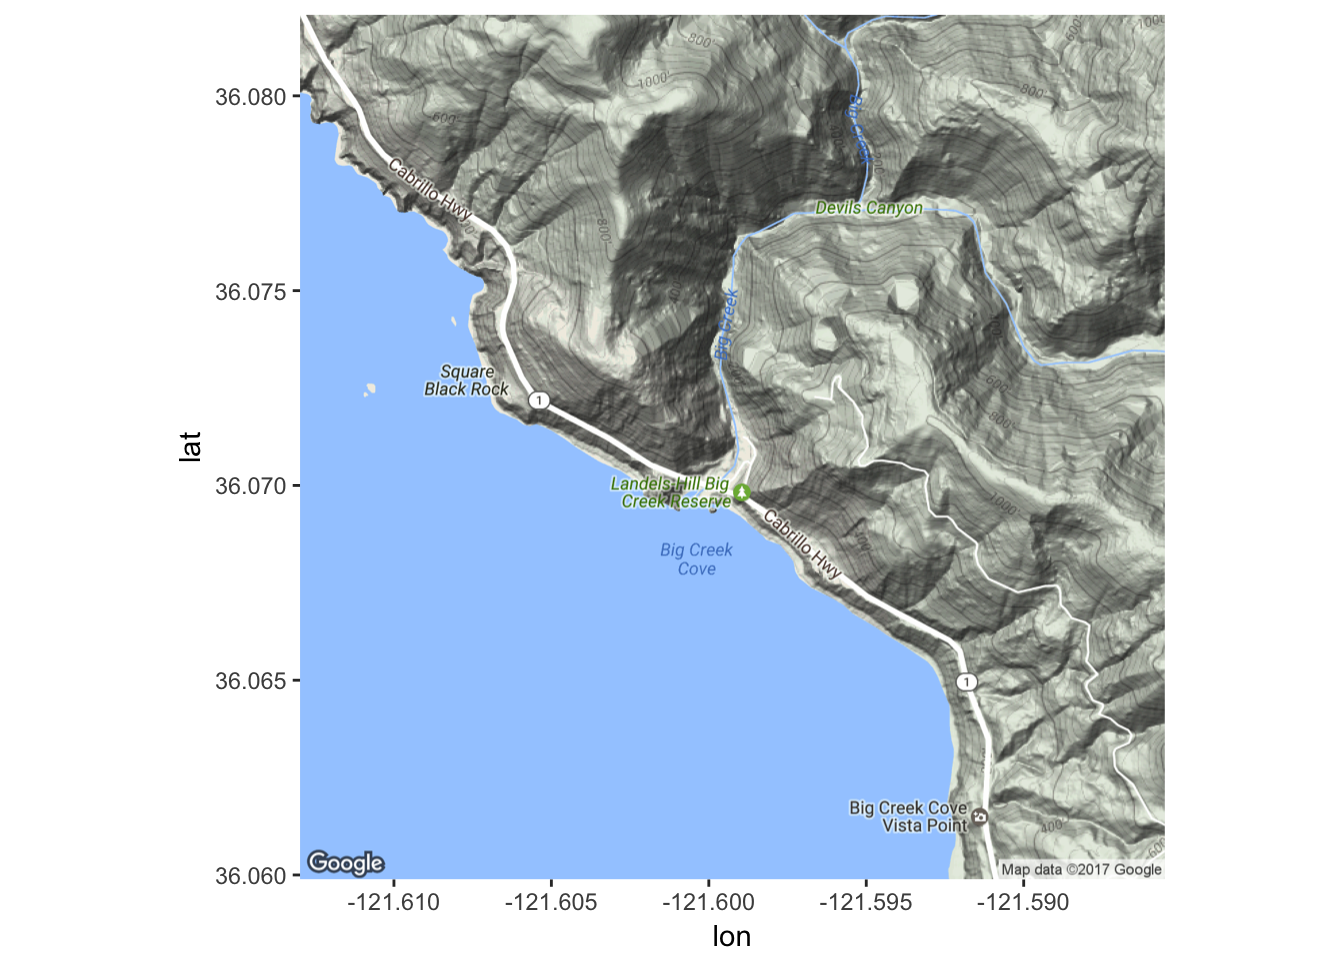
\includegraphics{bookdown-demo_files/figure-latex/unnamed-chunk-88-1.pdf}

Can we get the stamen maps to work?

\begin{Shaded}
\begin{Highlighting}[]
\NormalTok{bounds <-}\StringTok{ }\KeywordTok{c}\NormalTok{(}\DataTypeTok{left =} \NormalTok{-}\FloatTok{119.77}\NormalTok{, }
            \DataTypeTok{bottom =} \FloatTok{34.750}\NormalTok{,}
            \DataTypeTok{right =} \NormalTok{-}\FloatTok{119.73}\NormalTok{,}
            \DataTypeTok{top =} \FloatTok{34.755}\NormalTok{)}

\CommentTok{# note, if you get these in the wrong order you get a totally }
\CommentTok{# uninformative error message.}

\NormalTok{sisquoc_stamen <-}\StringTok{ }\KeywordTok{get_stamenmap}\NormalTok{(}\DataTypeTok{bbox =} \NormalTok{bounds, }\DataTypeTok{maptype =} \StringTok{"terrain"}\NormalTok{, }\DataTypeTok{zoom =} \DecValTok{16}\NormalTok{)}

\CommentTok{# this looks like crap!}

\CommentTok{# maybe at bigger zoom levels it would be OK.}
\end{Highlighting}
\end{Shaded}

\begin{itemize}
\item
  \texttt{ggmap} typically asks you for a zoom level, but we can try
  using \texttt{ggmap}'s \texttt{make\_bbox} function:

\begin{Shaded}
\begin{Highlighting}[]
\NormalTok{sbbox <-}\StringTok{ }\KeywordTok{make_bbox}\NormalTok{(}\DataTypeTok{lon =} \NormalTok{sisquoc$lon, }\DataTypeTok{lat =} \NormalTok{sisquoc$lat, }\DataTypeTok{f =} \NormalTok{.}\DecValTok{1}\NormalTok{)}
\NormalTok{sbbox}
\end{Highlighting}
\end{Shaded}

\begin{verbatim}
##       left     bottom      right        top 
## -119.76198   34.75111 -119.74201   34.75507
\end{verbatim}
\item
  Now, when we grab the map ggmap will try to fit it into that bounding
  box. Let's try:

\begin{Shaded}
\begin{Highlighting}[]
\CommentTok{# First get the map. By default it gets it from Google.  I want it to be a satellite map}
\NormalTok{sq_map <-}\StringTok{ }\KeywordTok{get_googlemap}\NormalTok{(}\DataTypeTok{location =} \NormalTok{sbbox, }\DataTypeTok{maptype =} \StringTok{"satellite"}\NormalTok{, }\DataTypeTok{source =} \StringTok{"google"}\NormalTok{)}
\end{Highlighting}
\end{Shaded}

\begin{verbatim}
## Source : https://maps.googleapis.com/maps/api/staticmap?center=29.763284,-95.363271&zoom=10&size=640x640&scale=2&maptype=satellite
\end{verbatim}

\begin{Shaded}
\begin{Highlighting}[]
\KeywordTok{ggmap}\NormalTok{(sq_map) +}\StringTok{ }\KeywordTok{geom_point}\NormalTok{(}\DataTypeTok{data =} \NormalTok{sisquoc, }\DataTypeTok{mapping =} \KeywordTok{aes}\NormalTok{(}\DataTypeTok{x =} \NormalTok{lon, }\DataTypeTok{y =} \NormalTok{lat), }\DataTypeTok{color =} \StringTok{"red"}\NormalTok{)}
\end{Highlighting}
\end{Shaded}

\begin{verbatim}
## Warning: Removed 8 rows containing missing values (geom_point).
\end{verbatim}

  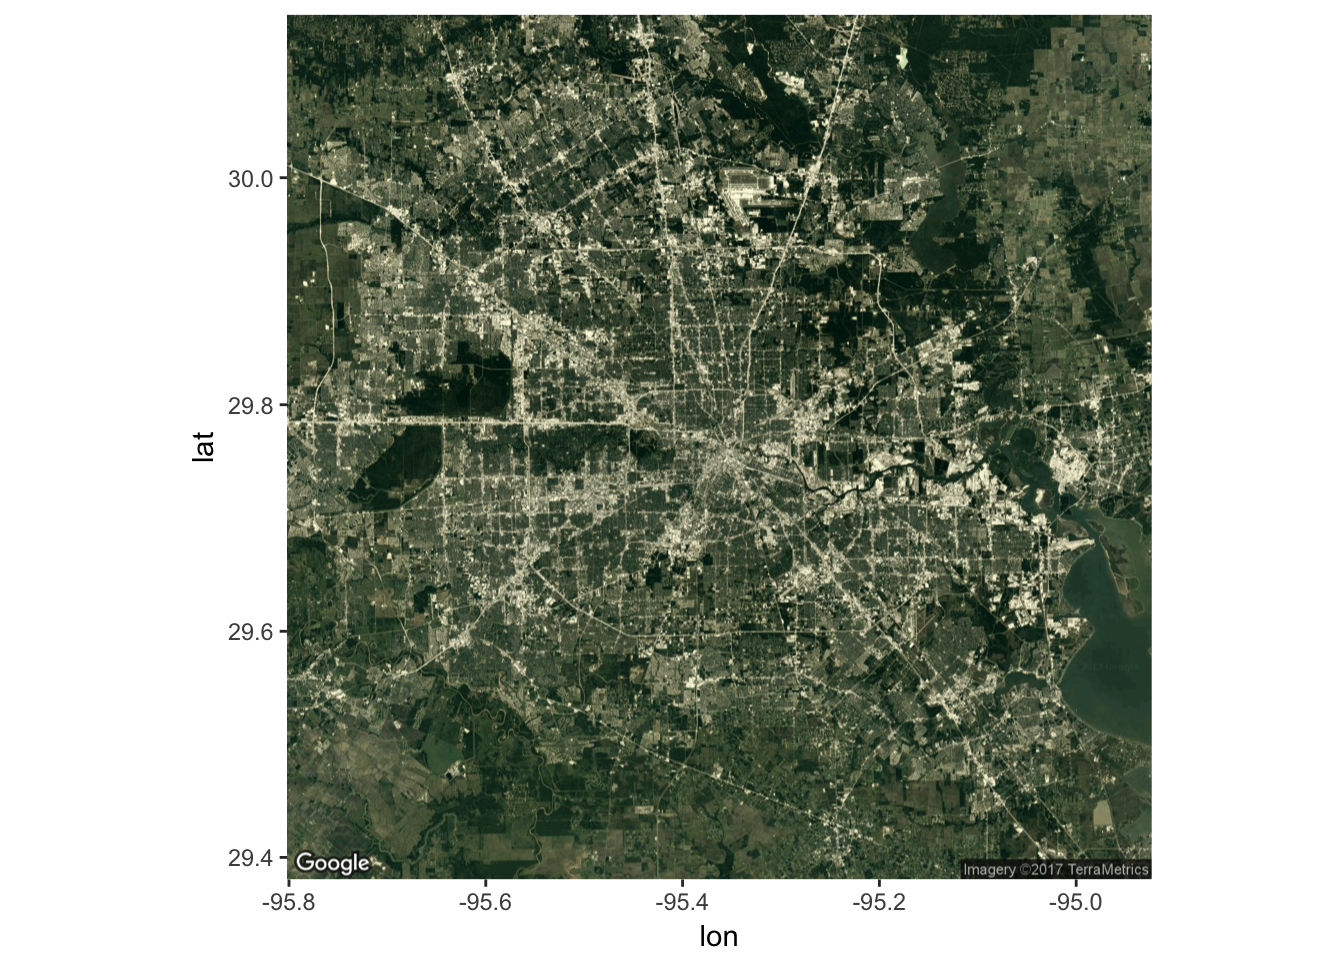
\includegraphics{bookdown-demo_files/figure-latex/unnamed-chunk-91-1.pdf}
\item
  Nope! That was a fail, but we got a warning about it too. (Actually it
  is a little better than before because I hacked \texttt{ggmap} a
  bit\ldots{}) Let's try using the zoom level. Zoom levels go from 3
  (world scale to 20 (house scale)).

\begin{Shaded}
\begin{Highlighting}[]
\CommentTok{# compute the mean lat and lon}
\NormalTok{ll_means <-}\StringTok{ }\KeywordTok{sapply}\NormalTok{(sisquoc[}\DecValTok{2}\NormalTok{:}\DecValTok{3}\NormalTok{], mean)}
\NormalTok{sq_map2 <-}\StringTok{ }\KeywordTok{get_map}\NormalTok{(}\DataTypeTok{location =} \NormalTok{ll_means,  }\DataTypeTok{maptype =} \StringTok{"satellite"}\NormalTok{, }\DataTypeTok{source =} \StringTok{"google"}\NormalTok{, }\DataTypeTok{zoom =} \DecValTok{15}\NormalTok{)}
\end{Highlighting}
\end{Shaded}

\begin{verbatim}
## Source : https://maps.googleapis.com/maps/api/staticmap?center=34.753117,-119.751324&zoom=15&size=640x640&scale=2&maptype=satellite&language=en-EN
\end{verbatim}

\begin{Shaded}
\begin{Highlighting}[]
\KeywordTok{ggmap}\NormalTok{(sq_map2) +}\StringTok{ }
\StringTok{  }\KeywordTok{geom_point}\NormalTok{(}\DataTypeTok{data =} \NormalTok{sisquoc, }\DataTypeTok{color =} \StringTok{"red"}\NormalTok{, }\DataTypeTok{size =} \DecValTok{4}\NormalTok{) +}
\StringTok{  }\KeywordTok{geom_text}\NormalTok{(}\DataTypeTok{data =} \NormalTok{sisquoc, }\KeywordTok{aes}\NormalTok{(}\DataTypeTok{label =} \KeywordTok{paste}\NormalTok{(}\StringTok{"  "}\NormalTok{, }\KeywordTok{as.character}\NormalTok{(name), }\DataTypeTok{sep=}\StringTok{""}\NormalTok{)), }\DataTypeTok{angle =} \DecValTok{60}\NormalTok{, }\DataTypeTok{hjust =} \DecValTok{0}\NormalTok{, }\DataTypeTok{color =} \StringTok{"yellow"}\NormalTok{)}
\end{Highlighting}
\end{Shaded}

  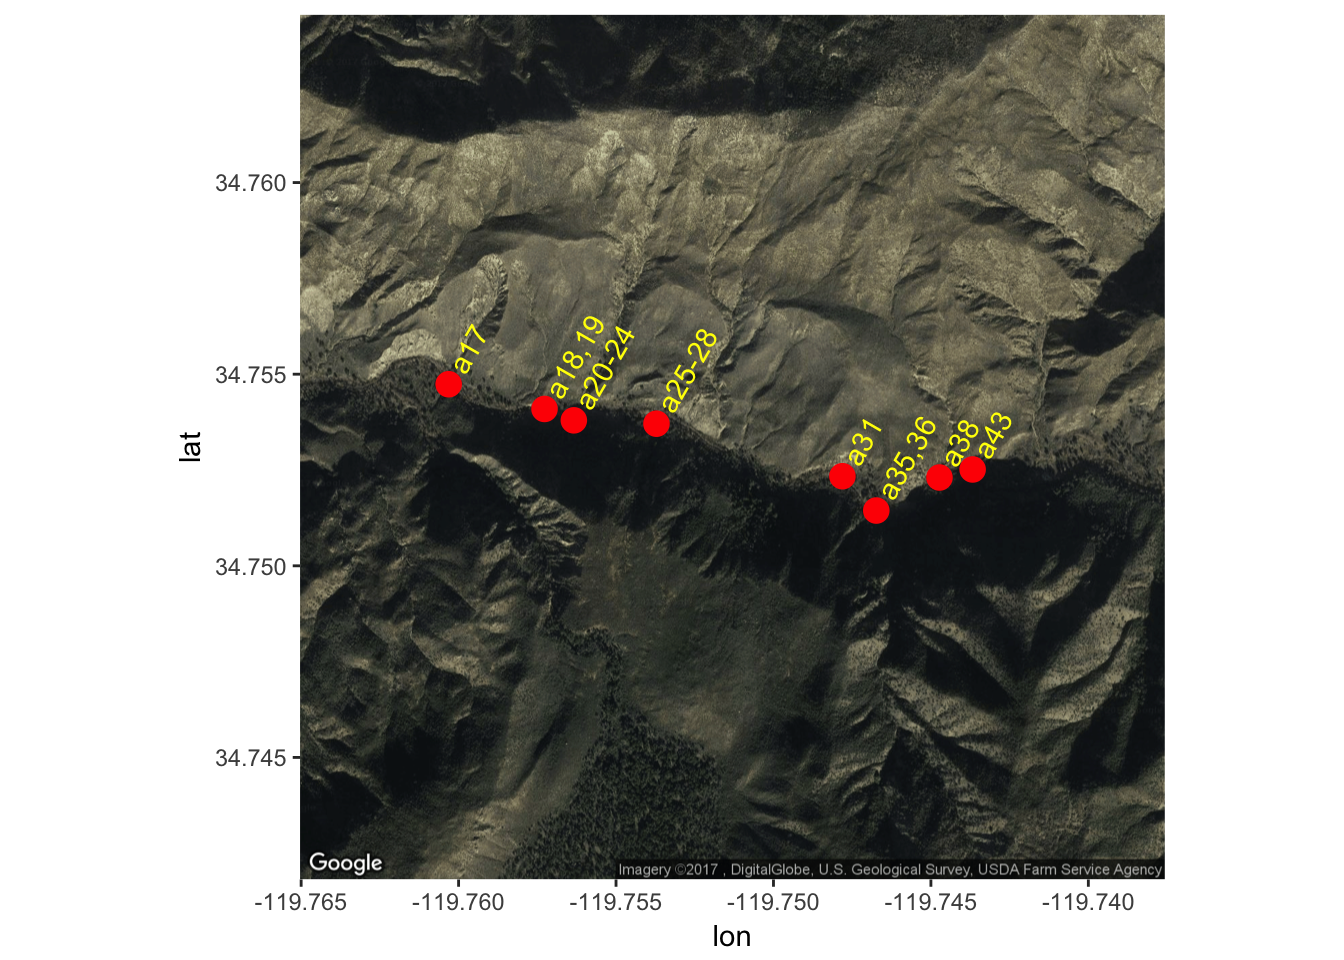
\includegraphics{bookdown-demo_files/figure-latex/unnamed-chunk-92-1.pdf}
\item
  That is decent. How about if we use the ``terrain'' type of map:

\begin{Shaded}
\begin{Highlighting}[]
\NormalTok{sq_map3 <-}\StringTok{ }\KeywordTok{get_map}\NormalTok{(}\DataTypeTok{location =} \NormalTok{ll_means,  }\DataTypeTok{maptype =} \StringTok{"terrain"}\NormalTok{, }\DataTypeTok{source =} \StringTok{"google"}\NormalTok{, }\DataTypeTok{zoom =} \DecValTok{15}\NormalTok{)}
\end{Highlighting}
\end{Shaded}

\begin{verbatim}
## Source : https://maps.googleapis.com/maps/api/staticmap?center=34.753117,-119.751324&zoom=15&size=640x640&scale=2&maptype=terrain&language=en-EN
\end{verbatim}

\begin{Shaded}
\begin{Highlighting}[]
\KeywordTok{ggmap}\NormalTok{(sq_map3) +}\StringTok{ }
\StringTok{  }\KeywordTok{geom_point}\NormalTok{(}\DataTypeTok{data =} \NormalTok{sisquoc, }\DataTypeTok{color =} \StringTok{"red"}\NormalTok{, }\DataTypeTok{size =} \DecValTok{4}\NormalTok{) +}
\StringTok{  }\KeywordTok{geom_text}\NormalTok{(}\DataTypeTok{data =} \NormalTok{sisquoc, }\KeywordTok{aes}\NormalTok{(}\DataTypeTok{label =} \KeywordTok{paste}\NormalTok{(}\StringTok{"  "}\NormalTok{, }\KeywordTok{as.character}\NormalTok{(name), }\DataTypeTok{sep=}\StringTok{""}\NormalTok{)), }\DataTypeTok{angle =} \DecValTok{60}\NormalTok{, }\DataTypeTok{hjust =} \DecValTok{0}\NormalTok{, }\DataTypeTok{color =} \StringTok{"yellow"}\NormalTok{)}
\end{Highlighting}
\end{Shaded}

  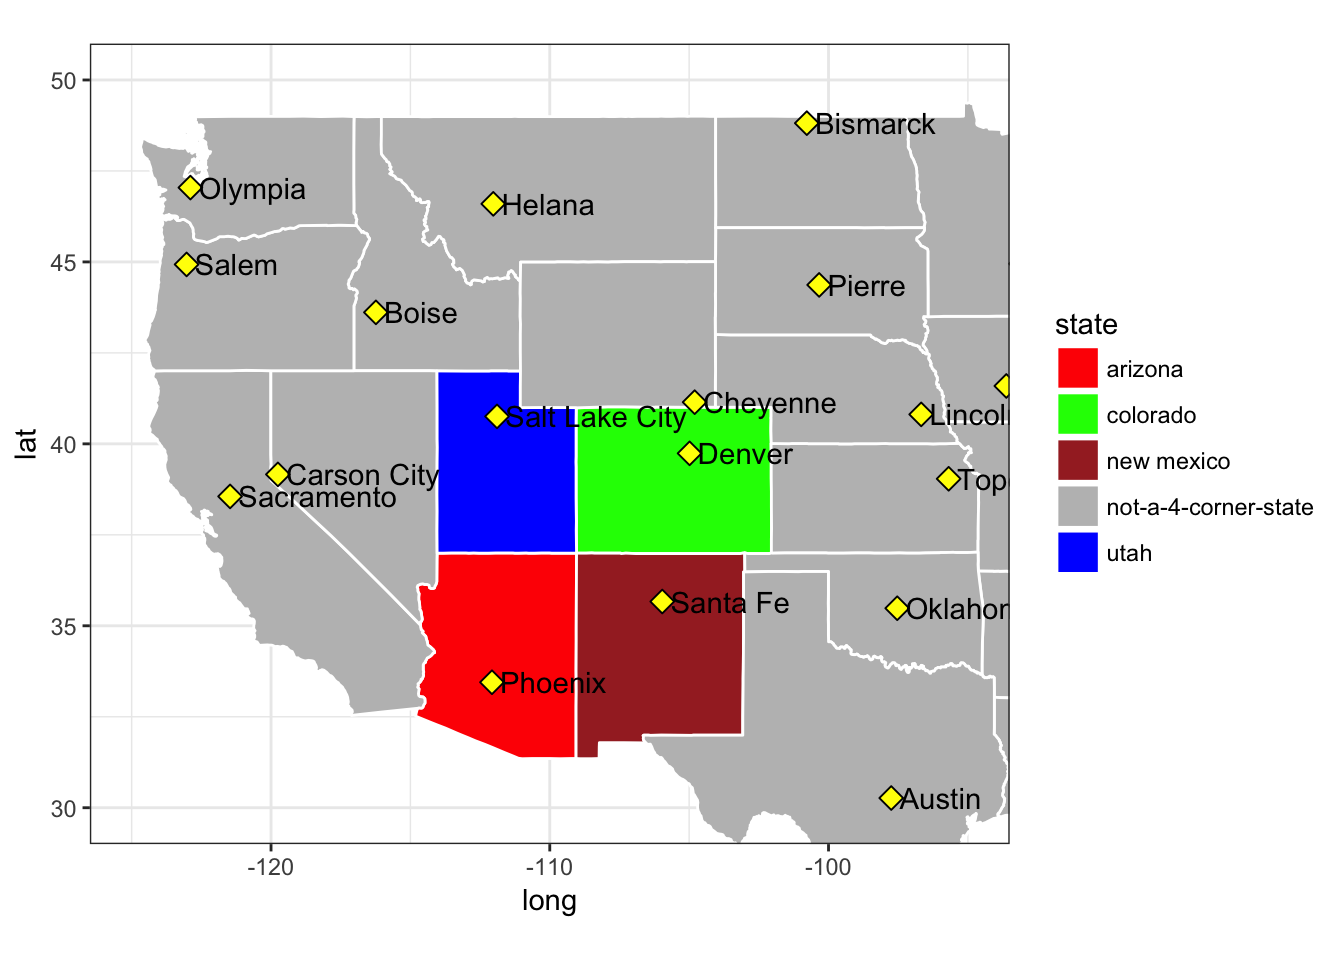
\includegraphics{bookdown-demo_files/figure-latex/unnamed-chunk-93-1.pdf}
\item
  That is cool, but I would search for a better color for the
  lettering\ldots{}
\end{itemize}

\subsection{How about a bike ride?}\label{how-about-a-bike-ride}

\begin{itemize}
\item
  I was riding my bike one day with a my phone and downloaded the GPS
  readings at short intervals.
\item
  We can plot the route like this:

\begin{Shaded}
\begin{Highlighting}[]
\NormalTok{bike <-}\StringTok{ }\KeywordTok{read.csv}\NormalTok{(}\StringTok{"inputs/bike-ride.csv"}\NormalTok{)}
\KeywordTok{head}\NormalTok{(bike)}
\end{Highlighting}
\end{Shaded}

\begin{verbatim}
##         lon      lat elevation                 time
## 1 -122.0646 36.95144      15.8 2011-12-08T19:37:56Z
## 2 -122.0646 36.95191      15.5 2011-12-08T19:37:59Z
## 3 -122.0645 36.95201      15.4 2011-12-08T19:38:04Z
## 4 -122.0645 36.95218      15.5 2011-12-08T19:38:07Z
## 5 -122.0643 36.95224      15.7 2011-12-08T19:38:10Z
## 6 -122.0642 36.95233      15.8 2011-12-08T19:38:13Z
\end{verbatim}

\begin{Shaded}
\begin{Highlighting}[]
\NormalTok{bikemap1 <-}\StringTok{ }\KeywordTok{get_map}\NormalTok{(}\DataTypeTok{location =} \KeywordTok{c}\NormalTok{(-}\FloatTok{122.080954}\NormalTok{, }\FloatTok{36.971709}\NormalTok{), }\DataTypeTok{maptype =} \StringTok{"terrain"}\NormalTok{, }\DataTypeTok{source =} \StringTok{"google"}\NormalTok{, }\DataTypeTok{zoom =} \DecValTok{14}\NormalTok{)}
\end{Highlighting}
\end{Shaded}

\begin{verbatim}
## Source : https://maps.googleapis.com/maps/api/staticmap?center=36.971709,-122.080954&zoom=14&size=640x640&scale=2&maptype=terrain&language=en-EN
\end{verbatim}

\begin{Shaded}
\begin{Highlighting}[]
\KeywordTok{ggmap}\NormalTok{(bikemap1) +}\StringTok{ }
\StringTok{  }\KeywordTok{geom_path}\NormalTok{(}\DataTypeTok{data =} \NormalTok{bike, }\KeywordTok{aes}\NormalTok{(}\DataTypeTok{color =} \NormalTok{elevation), }\DataTypeTok{size =} \DecValTok{3}\NormalTok{, }\DataTypeTok{lineend =} \StringTok{"round"}\NormalTok{) +}\StringTok{ }
\StringTok{  }\KeywordTok{scale_color_gradientn}\NormalTok{(}\DataTypeTok{colours =} \KeywordTok{rainbow}\NormalTok{(}\DecValTok{7}\NormalTok{), }\DataTypeTok{breaks =} \KeywordTok{seq}\NormalTok{(}\DecValTok{25}\NormalTok{, }\DecValTok{200}\NormalTok{, }\DataTypeTok{by =} \DecValTok{25}\NormalTok{))}
\end{Highlighting}
\end{Shaded}

  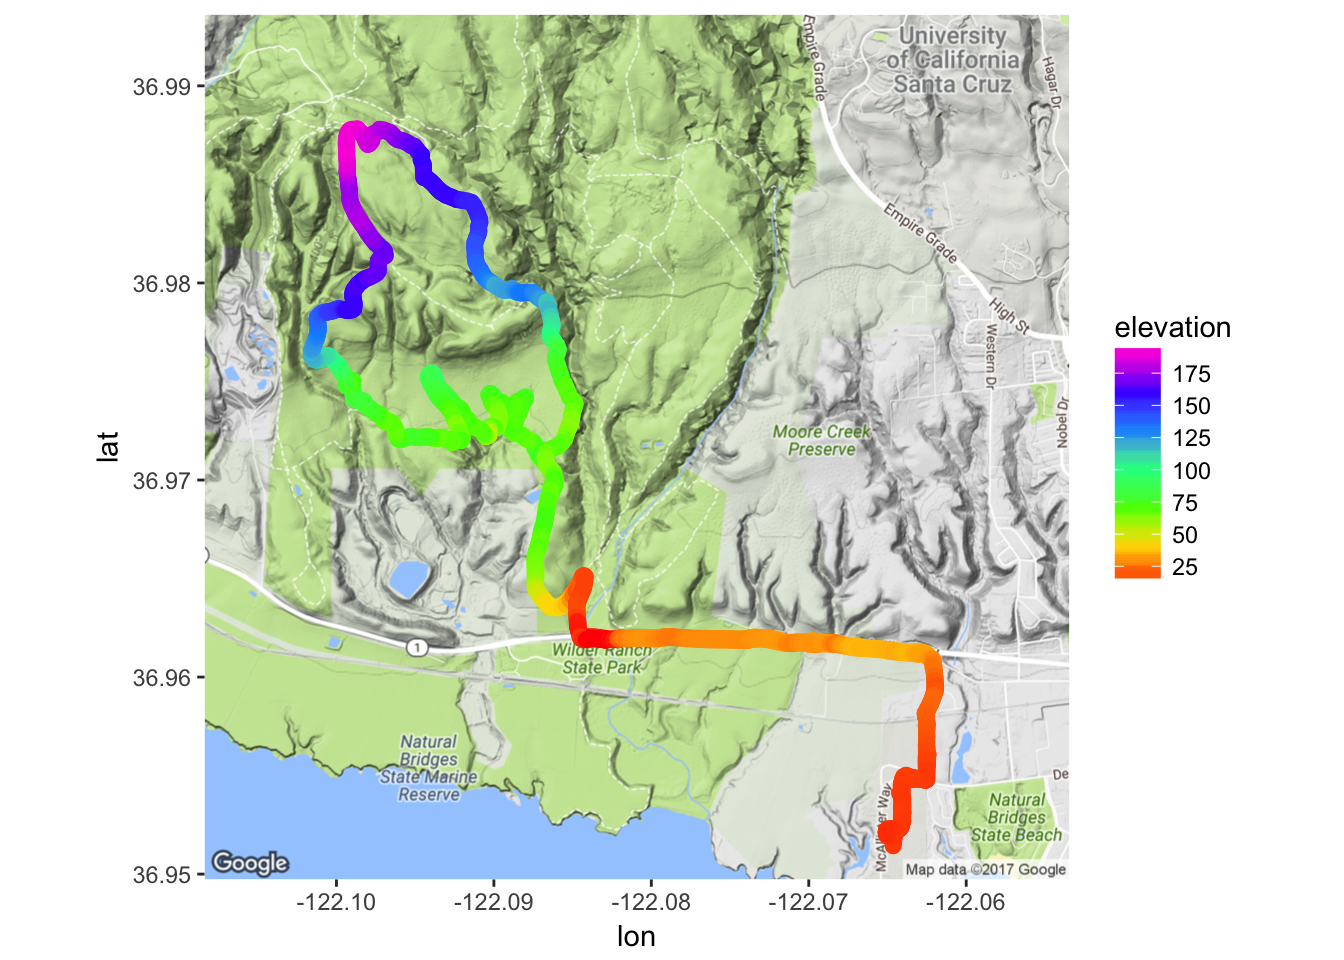
\includegraphics{bookdown-demo_files/figure-latex/unnamed-chunk-94-1.pdf}
\item
  See how we have mapped elevation to the color of the path using our
  rainbow colors again.
\item
  Note that getting the right zoom and position for the map is sort of
  trial and error. You can go to google maps to figure out where the
  center should be (right click and choose ``What's here?'' to get the
  lat-long of any point. )
\item
  The \texttt{make\_bbox} function has never really worked for me.
\end{itemize}

\subsection{Fish sampling locations}\label{fish-sampling-locations}

For this, I have whittled down some stuff in the coded wire tag data
base to georeferenced marine locations in British Columbia where at
least one Chinook salmon was recovered in between 2000 and 2012
inclusive. To see how I did all that you can check out
\href{https://github.com/eriqande/pbt-feasibility/blob/4ea2fc960f74f66b5ec3a11c107cdc52bfb346dc/Rmd/02-02-explore-recovery-and-catch-sample-data.Rmd\#looking-at-locations-of-location-codes}{this}

Let's have a look at the data:

\begin{Shaded}
\begin{Highlighting}[]
\NormalTok{bc <-}\StringTok{ }\KeywordTok{readRDS}\NormalTok{(}\StringTok{"inputs/bc_sites.rds"}\NormalTok{)}

\CommentTok{# look at some of it:}
\NormalTok{bc %>%}\StringTok{ }\KeywordTok{select}\NormalTok{(state_or_province:sub_location, longitude, latitude)}
\end{Highlighting}
\end{Shaded}

\begin{verbatim}
## # A tibble: 1,113 × 9
##    state_or_province water_type sector region  area location sub_location
##                <chr>      <chr>  <chr>  <chr> <chr>    <chr>        <chr>
## 1                  2          M      S     22  016   THOR IS           01
## 2                  2          M      N     26  012   MITC BY           18
## 3                  2          M      S     22  015   HARW IS           02
## 4                  2          M      N     26  006   HOPK PT           01
## 5                  2          M      S     23  017   TENT IS           06
## 6                  2          M      S     28  23A   NAHM BY           02
## 7                  2          M      N     26  006   GIL IS            06
## 8                  2          M      S     27  024   CLEL IS           06
## 9                  2          M      S     27  23B   SAND IS           04
## 10                 2          M      N     26  012   DUVA IS           16
## # ... with 1,103 more rows, and 2 more variables: longitude <dbl>,
## #   latitude <dbl>
\end{verbatim}

So, we have 1,113 points to play with.

\subsubsection{What do we hope to
learn?}\label{what-do-we-hope-to-learn}

\begin{itemize}
\item
  These locations in BC are hierarchically structured. I am basically
  interested in how close together sites in the same ``region'' or
  ``area'' or ``sector'' are, and pondering whether it is OK to
  aggregate fish recoveries at a certain level for the purposes of
  getting a better overall estimate of the proportion of fish from
  different hatcheries in these areas.
\item
  So, pretty simple stuff. I just want to plot these points on a map,
  and paint them a different color according to their sector, region,
  area, etc.
\item
  Let's just enumerate things first, using \texttt{dplyr}:

\begin{Shaded}
\begin{Highlighting}[]
\NormalTok{bc %>%}\StringTok{ }\KeywordTok{group_by}\NormalTok{(sector, region, area) %>%}\StringTok{ }\KeywordTok{tally}\NormalTok{()}
\end{Highlighting}
\end{Shaded}

\begin{verbatim}
## Source: local data frame [42 x 4]
## Groups: sector, region [?]
## 
##    sector region  area     n
##     <chr>  <chr> <chr> <int>
## 1             48  008      1
## 2             48  028      1
## 3             48  311      1
## 4       N     25  001     33
## 5       N     25  003     15
## 6       N     25  004     44
## 7       N     25  02E      2
## 8       N     25  02W     34
## 9       N     26  006     28
## 10      N     26  007     23
## # ... with 32 more rows
\end{verbatim}
\item
  That looks good. It appears like we could probably color code over the
  whole area down to region, and then down to area within subregions.
\end{itemize}

\subsubsection{Makin' a map.}\label{makin-a-map.}

\begin{itemize}
\tightlist
\item
  Let us try again to use \texttt{make\_bbox()} to see if it will work
  better when used on a large scale.
\end{itemize}

\begin{Shaded}
\begin{Highlighting}[]
\CommentTok{# compute the bounding box}
\NormalTok{bc_bbox <-}\StringTok{ }\KeywordTok{make_bbox}\NormalTok{(}\DataTypeTok{lat =} \NormalTok{latitude, }\DataTypeTok{lon =} \NormalTok{longitude, }\DataTypeTok{data =} \NormalTok{bc)}
\NormalTok{bc_bbox}
\end{Highlighting}
\end{Shaded}

\begin{verbatim}
##       left     bottom      right        top 
## -133.63297   47.92497 -122.33652   55.80833
\end{verbatim}

\begin{Shaded}
\begin{Highlighting}[]
\CommentTok{# grab the maps from google}
\NormalTok{bc_big <-}\StringTok{ }\KeywordTok{get_map}\NormalTok{(}\DataTypeTok{location =} \NormalTok{bc_bbox, }\DataTypeTok{source =} \StringTok{"google"}\NormalTok{, }\DataTypeTok{maptype =} \StringTok{"terrain"}\NormalTok{)}
\end{Highlighting}
\end{Shaded}

\begin{verbatim}
## Warning: bounding box given to google - spatial extent only approximate.
\end{verbatim}

\begin{verbatim}
## converting bounding box to center/zoom specification. (experimental)
\end{verbatim}

\begin{verbatim}
## Source : https://maps.googleapis.com/maps/api/staticmap?center=51.86665,-127.98475&zoom=6&size=640x640&scale=2&maptype=terrain&language=en-EN
\end{verbatim}

\begin{Shaded}
\begin{Highlighting}[]
\CommentTok{# plot the points and color them by sector}
\KeywordTok{ggmap}\NormalTok{(bc_big) +}\StringTok{ }
\StringTok{  }\KeywordTok{geom_point}\NormalTok{(}\DataTypeTok{data =} \NormalTok{bc, }\DataTypeTok{mapping =} \KeywordTok{aes}\NormalTok{(}\DataTypeTok{x =} \NormalTok{longitude, }\DataTypeTok{y =} \NormalTok{latitude, }\DataTypeTok{color =} \NormalTok{sector))}
\end{Highlighting}
\end{Shaded}

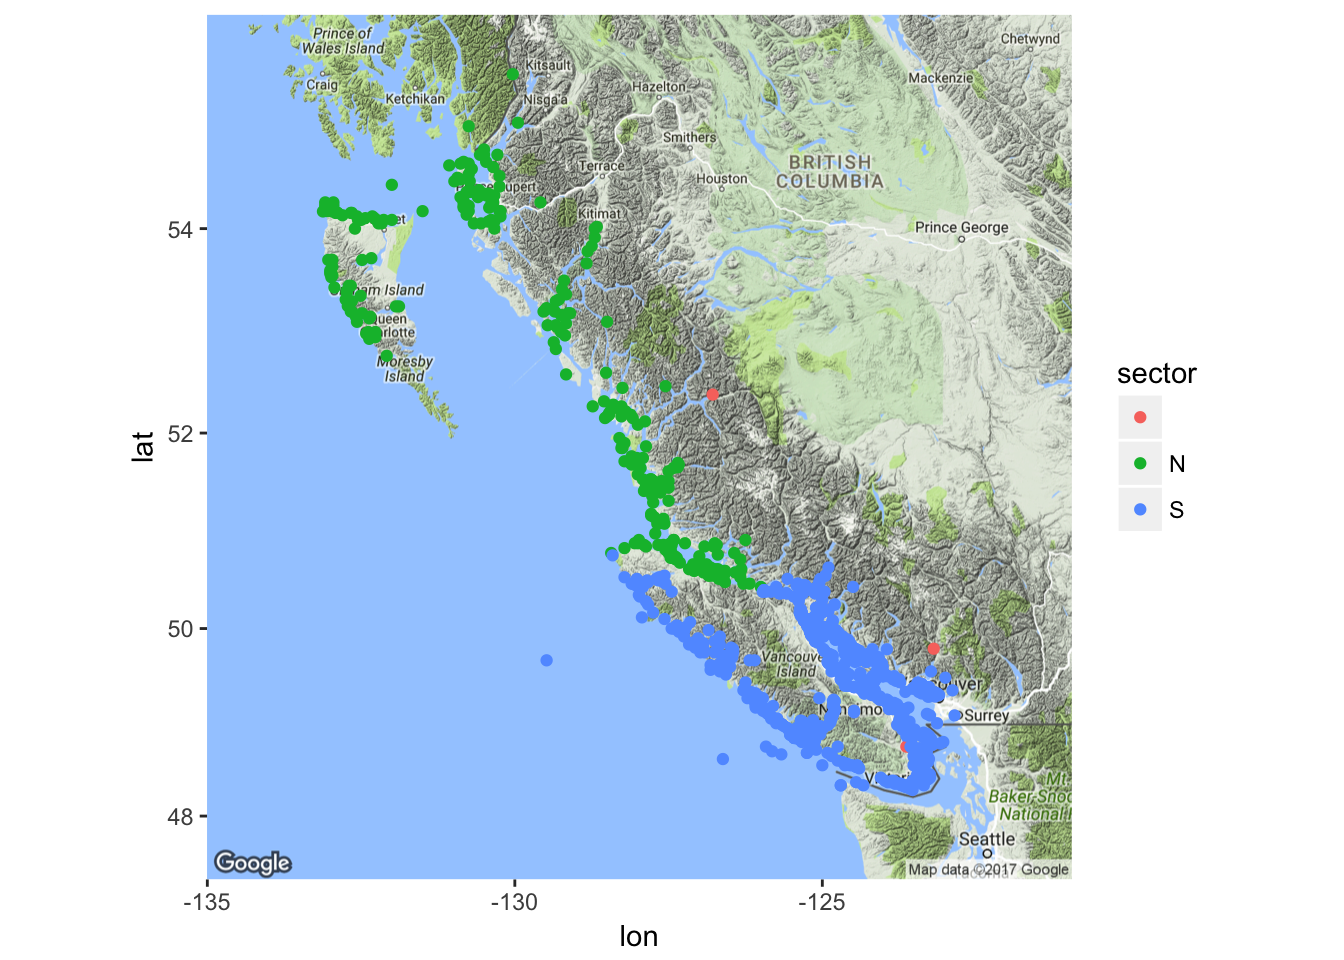
\includegraphics{bookdown-demo_files/figure-latex/unnamed-chunk-97-1.pdf}

\begin{itemize}
\tightlist
\item
  Cool! That was about as easy as could be. North is in the north, south
  is in the south, and the three reddish points are clearly aberrant
  ones at the mouths of rivers.
\end{itemize}

\subsubsection{Coloring it by region}\label{coloring-it-by-region}

\begin{itemize}
\tightlist
\item
  We should be able to color these all by region to some extent (it
  might get overwhelming), but let us have a go with it.
\item
  Notice that region names are unique overall (not just within N or S)
  so we can just color by region name.
\end{itemize}

\begin{Shaded}
\begin{Highlighting}[]
\KeywordTok{ggmap}\NormalTok{(bc_big) +}\StringTok{ }
\StringTok{  }\KeywordTok{geom_point}\NormalTok{(}\DataTypeTok{data =} \NormalTok{bc, }\DataTypeTok{mapping =} \KeywordTok{aes}\NormalTok{(}\DataTypeTok{x =} \NormalTok{longitude, }\DataTypeTok{y =} \NormalTok{latitude, }\DataTypeTok{color =} \NormalTok{region))}
\end{Highlighting}
\end{Shaded}

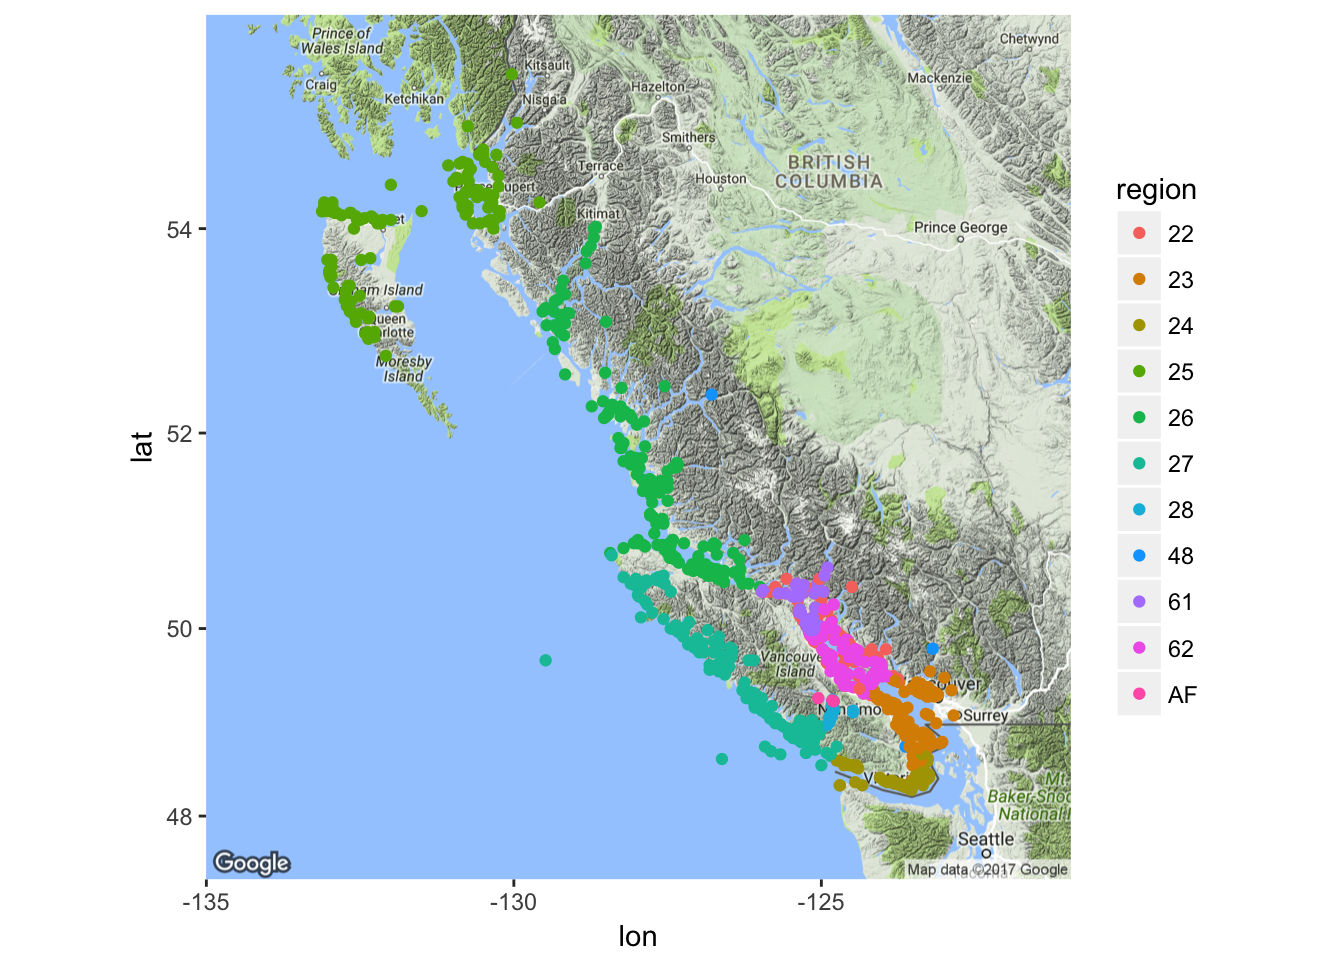
\includegraphics{bookdown-demo_files/figure-latex/unnamed-chunk-98-1.pdf}

\begin{itemize}
\tightlist
\item
  Once again that was dirt easy, though at this scale with all the
  different regions, it is hard to resolve all the colors.
\end{itemize}

\subsubsection{Zooming in on each region and coloring by
area}\label{zooming-in-on-each-region-and-coloring-by-area}

\begin{itemize}
\tightlist
\item
  It is time to really put this thing through its paces. (Keeping in
  mind that \texttt{make\_bbox()} might fail\ldots{})
\item
  I want to make series of maps. One for each region, in which the the
  areas in that region are colored differently.
\item
  How? Let's make a function: you pass it the region and it makes the
  plot.
\item
  Keep in mind that there are no factors in this data frame so we don't
  have to worry about dropping levels, etc.
\end{itemize}

\begin{Shaded}
\begin{Highlighting}[]
\NormalTok{region_plot <-}\StringTok{ }\NormalTok{function(MyRegion) \{}
  \NormalTok{tmp <-}\StringTok{ }\NormalTok{bc %>%}\StringTok{ }\KeywordTok{filter}\NormalTok{(region ==}\StringTok{ }\NormalTok{MyRegion)}
  \NormalTok{bbox <-}\StringTok{ }\KeywordTok{make_bbox}\NormalTok{(}\DataTypeTok{lon =} \NormalTok{longitude, }\DataTypeTok{lat =} \NormalTok{latitude, }\DataTypeTok{data =} \NormalTok{tmp)}
  \NormalTok{mymap <-}\StringTok{ }\KeywordTok{get_map}\NormalTok{(}\DataTypeTok{location =} \NormalTok{bbox, }\DataTypeTok{source =} \StringTok{"google"}\NormalTok{, }\DataTypeTok{maptype =} \StringTok{"terrain"}\NormalTok{)}
  \CommentTok{# now we want to count up how many areas there are}
  \NormalTok{NumAreas <-}\StringTok{ }\NormalTok{tmp %>%}\StringTok{ }\KeywordTok{summarise}\NormalTok{(}\KeywordTok{n_distinct}\NormalTok{(area))}
  \NormalTok{NumPoints <-}\StringTok{ }\KeywordTok{nrow}\NormalTok{(tmp)}
  
  \NormalTok{the_map <-}\StringTok{ }\KeywordTok{ggmap}\NormalTok{(mymap) +}
\StringTok{    }\KeywordTok{geom_point}\NormalTok{(}\DataTypeTok{data =} \NormalTok{tmp, }\DataTypeTok{mapping =} \KeywordTok{aes}\NormalTok{(}\DataTypeTok{x =} \NormalTok{longitude, }\DataTypeTok{y =} \NormalTok{latitude), }\DataTypeTok{size =} \DecValTok{4}\NormalTok{, }\DataTypeTok{color =} \StringTok{"black"}\NormalTok{) +}
\StringTok{    }\KeywordTok{geom_point}\NormalTok{(}\DataTypeTok{data =} \NormalTok{tmp, }\DataTypeTok{mapping =} \KeywordTok{aes}\NormalTok{(}\DataTypeTok{x =} \NormalTok{longitude, }\DataTypeTok{y =} \NormalTok{latitude, }\DataTypeTok{color =} \NormalTok{area), }\DataTypeTok{size =} \DecValTok{3}\NormalTok{) +}
\StringTok{    }\KeywordTok{ggtitle}\NormalTok{(}
      \KeywordTok{paste}\NormalTok{(}\StringTok{"BC Region: "}\NormalTok{, MyRegion, }\StringTok{" with "}\NormalTok{, NumPoints, }\StringTok{" locations in "}\NormalTok{, NumAreas, }\StringTok{" area(s)"}\NormalTok{, }\DataTypeTok{sep =} \StringTok{""}\NormalTok{)}
      \NormalTok{)}
  
  \KeywordTok{ggsave}\NormalTok{(}\KeywordTok{paste}\NormalTok{(}\StringTok{"bc_region"}\NormalTok{, MyRegion, }\StringTok{".pdf"}\NormalTok{, }\DataTypeTok{sep =} \StringTok{""}\NormalTok{), the_map, }\DataTypeTok{width =} \DecValTok{9}\NormalTok{, }\DataTypeTok{height =} \DecValTok{9}\NormalTok{)}
\NormalTok{\}}
\end{Highlighting}
\end{Shaded}

So, with that function we just need to cycle over the regions and make
all those plots.

Note that I am saving them to PDFs because it is no fun to make a web
page with all of those in there.

\begin{Shaded}
\begin{Highlighting}[]
\NormalTok{dump <-}\StringTok{ }\KeywordTok{lapply}\NormalTok{(}\KeywordTok{unique}\NormalTok{(bc$region), region_plot)}
\end{Highlighting}
\end{Shaded}

\chapter{in development}\label{in-development}

Yo! Here is info about the california hydrologic regions:

\url{https://www.arcgis.com/home/item.html?id=7a495cfa71ca4616aba58c5e915eef2c}

THey can be downloaded as shape files here
\url{https://mpsl.mlml.calstate.edu/GIS-shapefile-layers}.

\bibliography{packages.bib,book.bib}


\end{document}
